\documentclass{article}
\usepackage[english]{babel}
\usepackage{geometry,amsmath,graphicx,xcolor}
\geometry{letterpaper}

%%%%%%%%%% Start TeXmacs macros
\newcommand{\nobracket}{}
\newcommand{\tmaffiliation}[1]{\\ #1}
\newcommand{\tmcolor}[2]{{\color{#1}{#2}}}
\newcommand{\tmem}[1]{{\em #1\/}}
\newcommand{\tmmathbf}[1]{\ensuremath{\boldsymbol{#1}}}
\newcommand{\tmop}[1]{\ensuremath{\operatorname{#1}}}
\newcommand{\tmtextit}[1]{{\itshape{#1}}}
\newcommand{\tmtexttt}[1]{{\ttfamily{#1}}}
%%%%%%%%%% End TeXmacs macros

\begin{document}

\

\title{Notes on nonlinear gyrokinetic equation}

\author{
  Youjun Hu
  \tmaffiliation{Institute of Plasma Physics, Chinese Academy of Sciences\\
  Email: yjhu@ipp.cas.cn}
}

\maketitle

\begin{abstract}
  The nonlinear gyrokinetic equation given in Frieman-Chen's
  paper{\cite{frieman1982}} is re-derived in this note, providing more details
  on the derivation. The aspects that are relevant to numerical implementation
  of the gyrokinetic model are also discussed, which are actually the emphasis
  of this note.
\end{abstract}

\section{Introduction}

Subtle things in a theory, which may be crucial for one to fully understand
the theory, can be identified and understood only when one re-derives the
theory by oneself.

Presently, I do not understand the modern phase-space-Lagrangian Lie
perturbation method of deriving the gyrokinetic mode. So I am using the old
style asymptotic expansion method in deriving the gyrokinetic model, as was
done in the original Frieman-Chen's paper{\cite{frieman1982}}. \ The
motivation of deriving the gyrokinetic equation by myself is that I am
developing a new kinetic model in the \tmtexttt{GEM} code, which requires me
to understand every details of the gyrokinetic theory.

\section{Transform Vlasov equation from particle coordinates to guiding-center
coordinates}

To facilitate the derivation, we first need to choose some good variables to
work with (why they are good can only be realized when we get the results, but
some preliminary considerations can suggest that some variables be good).

The Vlasov equation in terms of particle coordinates $(\mathbf{x},
\mathbf{v})$ is given by
\begin{equation}
  \frac{\partial f_p}{\partial t} +\mathbf{v} \cdot \frac{\partial
  f_p}{\partial \mathbf{x}} + \frac{q}{m} (\mathbf{E}+\mathbf{v} \times
  \mathbf{B}) \cdot \frac{\partial f_p}{\partial \mathbf{v}} = 0,
\end{equation}
where $f_p = f_p (\mathbf{x}, \mathbf{v})$ is the particle distribution
function, $\mathbf{x}$ and $\mathbf{v}$ are the location and velocity of
particles. Next, we first define the guiding-center transformation. Then we
transform the Vlasov equation to the guiding-center coordinates, i.e., express
the gradient operators $\partial / \partial \mathbf{x}$ and $\partial /
\partial \mathbf{v}$ in terms of the guiding-center variables.

\subsection{Guiding-center transformation}

The transformation from the particle variables $(\mathbf{x}, \mathbf{v})$ to
the guiding-center variables $\mathbf{X}$ is defined by{\cite{Catto1978}}
\begin{equation}
  \label{16-9-21-1} \mathbf{X} (\mathbf{x}, \mathbf{v}) =\mathbf{x}+\mathbf{v}
  \times \frac{\tmmathbf{e}_{\parallel} (\mathbf{x})}{\Omega (\mathbf{x})},
\end{equation}
where $\mathbf{x}$ and $\mathbf{v}$ are particle position and velocity,
$\tmmathbf{e}_{\parallel} =\mathbf{B}_0 / B_0$, $\Omega = q B_0 / m$,
$\mathbf{B}_0 =\mathbf{B}_0 (\mathbf{x})$ is the equilibrium (macroscopic)
magnetic field at the particle position. It is obvious that $\tmmathbf{\rho}
\equiv -\mathbf{v} \times \mathbf{e}_{\parallel} / \Omega$ is the vector
gyro-radius pointing from the the guiding-center to the particle position.
This transformation involves both position and velocity of particles.

Given $(\mathbf{x}, \mathbf{v})$, it is straightforward to obtain $\mathbf{X}$
by using Eq. (\ref{16-9-21-1}). On the other hand, the inverse transformation,
i.e., given $(\mathbf{X}, \mathbf{v})$, to find $\mathbf{x}$. This is in
principle not easy because $\Omega$ and $\mathbf{e}_{\parallel}$ depend on
$\mathbf{x}$, which usually requires solving for the root of a nonlinear
equation. Numerically, one can use
\begin{equation}
  \label{18-9-13-p1} \mathbf{x}_{n + 1} =\mathbf{X}-\mathbf{v} \times
  \frac{\tmmathbf{e}_{\parallel} (\mathbf{x}_n)}{\Omega (\mathbf{x}_n)} .
\end{equation}
as an iteration scheme to compute $\mathbf{x}$. The initial guess can be
chosen as $\mathbf{x}_0 =\mathbf{X}$. The equilibrium magnetic field we will
consider has spatial scale length much larger than the thermal gyro radius
$\tmmathbf{\rho}$. In this case the difference between the values of
$\mathbf{e}_{\parallel} (\mathbf{x}) / \Omega (\mathbf{x})$ and
$\mathbf{e}_{\parallel} (\mathbf{X}) / \Omega (\mathbf{X})$ is small and thus
can be neglected. Then the inverse guiding-center transform can be written as
\begin{equation}
  \label{19-1-19-p2} \mathbf{x} \approx \mathbf{X}-\mathbf{v} \times
  \frac{\tmmathbf{e}_{\parallel} (\mathbf{X})}{\Omega (\mathbf{X})},
\end{equation}
which can also be considered as we using the iterative scheme
(\ref{18-9-13-p1}) to computer $\mathbf{x}$ and stopping at the first
iteration. The difference between equilibrium field values evaluated at
$\mathbf{X}$ and $\mathbf{x}$ is always neglected in gyrokinetic theory.
Therefore it does not matter whether the above $\mathbf{e}_{\parallel} /
\Omega$ is evaluated at $\mathbf{x}$ or $\mathbf{X}$. What matters is where
the perturbed fields are evaluated: at $\mathbf{x}$ or at $\mathbf{X}$. The
values of perturbed fields at $\mathbf{x}$ or at $\mathbf{X}$ are different
and this is called the finite Larmor radius (FLR) effect, which is almost all
that the gyrokinetic theory is about.

\subsection{Gyro-angle}

The forward and backward guiding-center transformations (\ref{16-9-21-1}) and
(\ref{19-1-19-p2}) involve the velocity vector $\mathbf{v}$. It is the cross
product between $\mathbf{v}$ and $\tmmathbf{e}_{\parallel} (\mathbf{x})$ or
$\tmmathbf{e}_{\parallel} (\mathbf{X})$ that is actually used. Therefore, only
two of the three coordinates of $\mathbf{v}$ is actually needed in a local (at
$\mathbf{x}$ or $\mathbf{X}$) cylindrical coordinate system, namely
$v_{\perp}$ and $\alpha$, where $\alpha$ is the azimuthal angle of the
velocity in the local cylindrical system. Here $\alpha$ will be called the
gyro-phase or gyro-angle in the following.

\subsection{Distribution functions in terms of guiding-center variables}

Denote the distribution function in terms of the guiding-center variables
$(\mathbf{X}, \mathbf{v})$ by $f_g (\mathbf{X}, \mathbf{v})$, then the
relation between $f_g$ and $f_p$ is given by
\begin{equation}
  \label{17-8-19-p1} f_g (\mathbf{X}, \mathbf{v}) = f_p (\mathbf{x},
  \mathbf{v}),
\end{equation}
where $\mathbf{X}$ and $\mathbf{x}$ are related to each other via Eq.
(\ref{16-9-21-1}). Equation (\ref{17-8-19-p1}) along with Eq.
(\ref{16-9-21-1}) can be considered as the definition of the guiding-center
distribution function $f_g$. Using Eq. (\ref{16-9-21-1}), the above relation
can be equivalently written as
\begin{equation}
  \label{17-5-15-p11} f_g (\mathbf{X}, \mathbf{v}) = f_p
  (\mathbf{X}+\tmmathbf{\rho}, \mathbf{v}),
\end{equation}
or
\begin{equation}
  \label{17-8-19-p3} f_p (\mathbf{x}, \mathbf{v}) = f_g
  (\mathbf{x}-\tmmathbf{\rho}, \mathbf{v}) .
\end{equation}
or $f_p (\mathbf{x}, \mathbf{v}) = f_p (\mathbf{X}+\tmmathbf{\rho},
\mathbf{v})$, or $f_g (\mathbf{X}, \mathbf{v}) = f_g
(\mathbf{x}-\tmmathbf{\rho}, \mathbf{v})$.

As is conventionally adopted in multivariables calculus, both $f_p$ and $f_g$
are sometimes simply denoted by $f$. Which one is actually assumed depends on
the context, i.e., depends on which independent variables are actually
assumed: particle variables or guiding-center variables. This is one of the
subtle (trivial?) things needed to be noted for gyrokinetic theory in
particular and for multivariables calculus in general. This notation will
cause confusions when, for example, $f_g (\mathbf{X}, \mathbf{v})$ is
evaluated at $\mathbf{X}=\mathbf{x}$, i.e., $f_g (\mathbf{x}, \mathbf{v})$,
which, if the subscript $g$ is omitted and we rely on dependent variables to
identify whether it is $f_p$ or $f_g$, will be wrongly understood as $f_p$.
Therefore it seems better to use the accurate notation. One example where this
distinguishing is important is encountered when we try to express the
diamagnetic flow in terms of $f_g$, which is discussed in Appendix
\ref{17-8-19-e1}.

In practice, $f_g$ is often called the guiding-center distribution function
whereas $f_p$ is called the particle distribution function. They are the same
distribution function expressed in different variables.

In the above, we assume that $\mathbf{X}$ and $\mathbf{x}$ are always related
to each other by the guiding-center transformation (\ref{16-9-21-1}) or
(\ref{19-1-19-p2}) , i.e., $\mathbf{x}$ and $\mathbf{X}$ are not independent.
For some cases, it may be convienent to treat $\mathbf{x}$ and $\mathbf{X}$ as
independent variables and express the guiding-center transformation via an
integral of the Dirac delta function. For example, expression
(\ref{17-8-19-p3}) can be written as
\begin{equation}
  \label{19-1-20-e1} f_p (\mathbf{x}, \mathbf{v}) = \int f_g (\mathbf{X},
  \mathbf{v}) \delta^3 (\mathbf{X}-\mathbf{x}+\tmmathbf{\rho}) d\mathbf{X},
\end{equation}
where $\mathbf{x}$ and $\mathbf{X}$ are considered as independent variables,
$\delta^3 (\mathbf{x}-\mathbf{X}-\tmmathbf{\rho})$ is the three-dimensional
Dirac delta function. [In terms of general coordinates $(x_1, x_2, x_3)$, the
three-dimensional Dirac delta function is defined via the 1D Dirac delta
function as follows:
\begin{equation}
  \delta^3 (\mathbf{x}) = \frac{1}{| \mathcal{J} |} \delta (x_1) \delta (x_2)
  \delta (x_3),
\end{equation}
where $\mathcal{J}$ is the the Jacobian of the general coordinate system. The
Jacobian is included in order to make $\delta^3 (\mathbf{x})$ satisfy the
normalization condition $\int \delta^3 (\mathbf{x}) d\mathbf{x}= \int \delta^3
(\mathbf{x}) | \mathcal{J} | d x_1 d x_2 d x_3 = 1$.]

Expression (\ref{19-1-20-e1}) can be considered as a transformation that
transforms an arbitrary function from the guiding-center coordinates to the
particle coordinates. Similarly, equation (\ref{17-5-15-p11}) can be written
as
\begin{equation}
  f_g (\mathbf{X}, \mathbf{v}) = \int f_p (\mathbf{x}, \mathbf{v}) \delta^3
  (\mathbf{x}-\mathbf{X}-\tmmathbf{\rho}) d\mathbf{x},
\end{equation}
which can be considered as a transformation that transforms an arbitrary
function from the the particle coordinates to the guiding-center coordinates.

\subsection{Moments of distribution function expressed as integration over
guiding-center variables}

In terms of particle variables $(\mathbf{x}, \mathbf{v})$, it is
straightforward to calculate the moment of the distribution function. For
example, the number density $n (\mathbf{x})$ is given by
\begin{equation}
  \label{18-12-26-p1} n (\mathbf{x}) = \int f_p (\mathbf{x}, \mathbf{v})
  d\mathbf{v}.
\end{equation}
However, it is a little difficult to calculate $n (\mathbf{x})$ at real space
location $\mathbf{x}$ by using the guiding-center variables $(\mathbf{X},
\mathbf{v})$. This is because holding $\mathbf{x}$ constant and changing
$\mathbf{v}$, as required by the integration in Eq. (\ref{18-12-26-p1}), means
the guiding-center variable $\mathbf{X}$ is changing, according to Eq.
(\ref{16-9-21-1}). Using Eq. (\ref{17-8-19-p1}), expression
(\ref{18-12-26-p1}) is written as
\begin{equation}
  \label{18-12-26-p2} n (\mathbf{x}) = \int f_g (\mathbf{X} (\mathbf{x},
  \mathbf{v}), \mathbf{v}) d\mathbf{v},
\end{equation}
As is mentioned above, the $d\mathbf{v}$ integration in Eq.
(\ref{18-12-26-p2}) should be performed by holding $\mathbf{x}$ constant and
changing $\mathbf{v}$, which means the guiding-center variable
$\mathbf{X}=\mathbf{X} (\mathbf{x}, \mathbf{v})$ is changing. This means that,
in $(\mathbf{X}, \mathbf{v})$ space, the above integration is a (generalized)
line integral along the the line $\mathbf{X} (\mathbf{v})
=\mathbf{x}-\tmmathbf{\rho} (\mathbf{x}, \mathbf{v})$ with $\mathbf{x}$ being
constant. By using the Dirac delta function $\delta$, this line integral can
be written as the following two-dimensional integration over the independent
variables $\mathbf{X}$ and $\mathbf{v}$:
\begin{equation}
  \label{19-1-19-p1} n (\mathbf{x}) = \int \int f_g (\mathbf{X}, \mathbf{v})
  \delta^3 (\mathbf{X}-\mathbf{x}+\tmmathbf{\rho}) d\mathbf{v}d\mathbf{X}.
\end{equation}
In gyrokinetic particle in cell (PIC) simulations, the integral
(\ref{19-1-19-p1}) is evaluated by using Monte-Carlo markers. Actually
evaluated in the simulation is the integral of a special $f_g$ that is
independent of the gyro-angle $\alpha$. Using $v_{\perp}$ and $v_{\parallel}$
as the two remaining velocity coordinates, then $f_g$ is written as $f_g = f_g
(\mathbf{X}, v_{\perp}, v_{\parallel})$. In this case $f_g$ is a function of
five variables (rather than six variables).

In simulations, the position of a marker represents the guiding-center
location (rather than the particle location), i.e., it is the guiding-center
location that is directly sampled (the particle position is indirectly
sampled, as is discussed below). For a marker with coordinators $(\mathbf{X},
v_{\perp}, v_{\parallel})$, we can calculate particle positions by using the
transformation (\ref{19-1-19-p2}). There are infinite number of particle
positions associated with the marker since the direction of $v_{\perp}$ (i.e.,
gyro-agnle) is not specified. All these possible particle positions are on a
circle around the guiding-center position $\mathbf{X}$. This circle is often
called the gyro-ring. In particle simulations, the gyro-ring is descretized by
several sampling points in calculating its integration contribution to grids.
We choose $N$ sampling points that are evenly distributed on the gyro-ring
($N$ is usually $4$ as a compromise between efficiency and accuracy). Denote
the Mote-Carlo weight of the $j \tmop{th}$ marker by $w_j$. Then the weight is
evenly split by the $N$ sub-markers on the gyro-ring since $f_g (\mathbf{X},
v_{\perp}, v_{\parallel})$ is independent of the gyro-phase (put it another
way, $f_g$ is uniformed distributed in the gyro-phase) Therefore each
sub-marker have a Monte-Carlo weight $w_j / N$. Then calculating the
integration (\ref{19-1-19-p1}) at a grid corresponds to depositing all the $N$
sub-markers associated with each guiding-center marker to the grid, as is
illustrated in Fig. \ref{19-1-19-p4}. A more accurate interpretation of why
the charge deposition can be done this way is discussed in Sec.
\ref{19-1-28-1}.

\begin{figure}[h]
  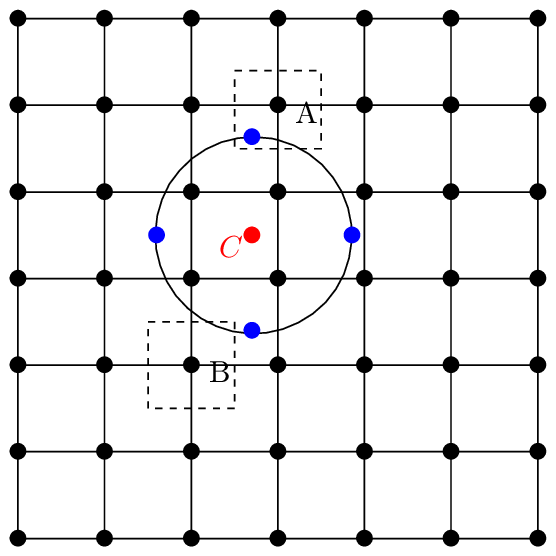
\includegraphics{/home/yj/theory/figures/grids_cells/grids-3.eps}
  \caption{\label{19-1-19-p4}The spatial grids in the plane perpendicular to
  the equilibrium magnetic field and one gyro-ring with \tmcolor{blue}{4
  sampling points} (sub-markers) on it. For a guiding-center marker $C$ with a
  Monte-Carlo weight of $w_j$, the 4 sub-markers are calculated by using the
  transformation (\ref{19-1-19-p2}) (rebuilding the gyro-ring). The
  Monte-Carlo weight of each sub-marker is $w_j / 4$. The value of integration
  (\ref{19-1-19-p1}) at a grid point is approximated by $I / \Delta V$, where
  $I$ is the Monte-Carlo integration of all sub-markers associated with all
  guiding-center markers in the cell, $\Delta V$ is the cell volume. The cell
  associated with a grid-point (e.g., $A$) is indicated by the dashed
  rectangle (this is for 2D case, for 3D, it is a cube). If the Dirac delta
  function is used as the shape function of the sub-markers, then calculating
  the contribution of a sub-marker to a grid corresponds to the nearest-point
  interpolation (for example, the 4 sub-markers will contribute noting to grid
  $B$ since no-sub marker is located within the cell). In practice, the
  flat-top shape function with its support equal to the cell size is often
  used, then the depositing corresponds to linearly interpolating the weight
  of each sub-marker to the nearby grids.}
\end{figure}

\

The gyro-averaging of a perturbed field can be numerically calculated in a
way similar to the above (discussed later).

\subsection{Monte-Carlo sampling of 6D guiding-center phase-space
}\label{19-1-28-1}

Suppose that the 6D guiding-center phase-space $(\mathbf{X}, \mathbf{v})$ is
described by $(\psi, \theta, \phi, v_{\parallel}, v_{\perp}, \alpha)$
coordinates. The Jacobian of the coordinate system is given by $\mathcal{J} =
\mathcal{J}_r v_{\perp} \mathcal{}$, where $\mathcal{J}_r$ is the Jacobian of
$(\psi, \theta, \phi)$ coordinates. Suppose that we sample the 6D phase-space
by using the following probability density function:
\begin{equation}
  \label{19-1-26-1} P (\psi, \theta, \phi, v_{\parallel}, v_{\perp}, \alpha) =
  \frac{1}{V_r} \left( \frac{m}{2 \pi T} \right)^{3 / 2} \exp \left[ - \frac{m
  (v_{\parallel}^2 + v_{\perp}^2)}{2 T} \right],
\end{equation}
where $V_r$ is the volume of the spatial simulation box, $T$ is a constant
temperature. ($P$ given above is actually independent of $\psi, \theta, \phi$
and $\alpha$.) It is ready to verify that $P$ satisfies the following
normalization condition:
\begin{equation}
  \int_{V_r} \int P d\mathbf{v}d\mathbf{X}= \int_{V_r} \int_{- \infty}^{+
  \infty} \int_0^{\infty} \int_0^{2 \pi} P v_{\perp} d \alpha d v_{\perp} d
  v_{\parallel} \mathcal{J}_r d \psi d \theta d \phi = 1.
\end{equation}
We use the rejection method to numerically generate $N_p$ markers that satisfy
the above probability density function. [The effective probability density
function actually used in the rejection method is $P'$, which is related to
$P$ by
\begin{equation}
  P' = | \mathcal{J}_r \mathcal{J}_v | P = | \mathcal{J}_r | v_{\perp} P.
\end{equation}
Note that $P'$ does not depend on the gyro-angle $\alpha$.] Then the
phase-space volume occupied by a marker is given by
\begin{equation}
  V_{p j} = \frac{1}{g} = \frac{1}{N_p P} = \frac{V_r}{N_p \left( \frac{m}{2
  \pi T} \right)^{3 / 2} \exp \left[ - \frac{m (v_{\parallel j}^2 + v_{\perp
  j}^2)}{2 T} \right]},
\end{equation}
which is independent of $\psi_j, \theta_j, \phi_j$ and $\alpha_j$. The weight
of a marker is then given by $w_j = V_{p j} \delta f_{g j}$, where $\delta
f_g$ is the perturbed distribution function evolved in simulations.

Although the distribution function $\delta f_g$ to be sampled in gyrokinetic
simulations is independent of the gyro-angle $\alpha$, we still need to sample
the gyro-angle because we need to use the inverse guiding-center
transformation, which needs the gyro-angle. Each marker needs to have a
specific gyro-angle value $\alpha_j$ so that we know how to transform its
$\mathbf{X}_j$ to $\mathbf{x}_j$ and then do the charge deposition in
$\mathbf{x}$ space. To increase the resolution over the gyro-angle, we need to
increase the number of markers. However, thanks to the fact that both sampling
probability density function $P$ and $\delta f_g$ are independent of $\alpha$,
the resolution over the gyro-angle can be increased in a simple way.
Specifically, for a marker with $(\mathbf{X}_j, v_{\parallel j}, v_{\perp
j})$, its gyro-angle value $\alpha_j$ can be adjusted arbitrary without
changing the value of its weight $w_j$ because both the phase-space volume
$V_{p j}$ and $\delta f_{g j}$ are independent of $\alpha_j$. In other words,
we have the freedom of choosing the value of $\alpha_j$ and the independence
of $V_{p j}$ and $\delta f_{g j}$ on $\alpha_j$ guarantees that the weight of
the marker is still equal to the original value that this marker takes.
Suppose that we choose $4$ different values of $\alpha_j$ for the $j
\tmop{th}$ marker, denoted by $\alpha_{j 1}$, $\alpha_{j 2}$, $\alpha_{j 3}$,
and $\alpha_{j 4}$. Then for each of the four gyro-angle values, we do the
inverse guiding-center transformation and then do the charge deposition using
their original weight $w_j$ for each marker and then loop over all the
markers. Denote a grid quantity (e.g. density) build by the deposition process
by $n_1 (\mathbf{x})$, $n_2 (\mathbf{x})$, $n_3 (\mathbf{x})$, and $n_4
(\mathbf{x})$, corresponding to using the four gyro-angle values. Then the
more accurate estimation of the grid quantity is given by
\begin{equation}
  n (\mathbf{x}) = \frac{n_1 (\mathbf{x}) + n_2 (\mathbf{x}) + n_3
  (\mathbf{x}) + n_4 (\mathbf{x})}{4} .
\end{equation}
This corresponds to sampling the 6D phase-space 4 separate times (each time
with identical sampling points in $(\mathbf{X}, v_{\parallel}, v_{\perp})$ but
different sampling points in $\alpha$) and then using the averaging of the 4
Monte-Carlo integrals to estimate the exact value. This estimation can also be
(roughly) considered as a Monte-Carlo estimation using 4 times larger number
of markers as that is originally used (the Monte-Carlo estimation using truly
4 time larger number of markers is more accurate than the result we obtained
above because the former also increase the resolution of $(\mathbf{X},
v_{\parallel}, v_{\perp})$ while the latter keeps the resolution of
$(\mathbf{X}, v_{\parallel}, v_{\perp})$ unchanged.)

In numerical code, one may split the weight $w_j$ as $w_j / 4$ in doing the
deposition and then add the contributions from all the 4 gyro-angles when
doing the deposition and then one does not need to take the averaging at the
end. However, interpreting in this way is confusing to me because, with a
single sampling of the phase-space, the phase-space volume or weight can not
be easily split. I prefer the above interpretation that the 6D phase space is
sampled 4 separate times and thus we get 4 estimations and finally we take the
averaging of these 4 estimations. It took me several days to finally find this
way of understanding.

In summary, the phase-space to be sampled in gyrokinetic simulations are still
6D rather than 5D. In this sense, the statement that gyrokinetic simulation
works in a 5D phase space is misleading. We are still working in the 6D
phase-space. The only subtle thing is that the sixth dimension, i.e.,
gyro-angle, can be sampled in a easy way that is independent of the other 5
variables.

In numerical implementation, the gyro-angle may not be explicitly used. We
just try to calculate 4 arbitrary points on the gyro-ring that are easy to
calculate. Some codes (e.g. ORB5) may introduce a random variable to rotate
these 4 points for different markers so that the gyro-angle is sampled more
unbiased.

\subsection{Choosing velocity coordinates}

Coordinates of the velocity space can be chosen as $(v, v_{\parallel},
\alpha)$, or $(v, v_{\perp}, \alpha)$, or $(v_{\parallel}, v_{\perp},
\alpha)$, where $v_{\parallel}$ and $v_{\perp}$ are the parallel and
perpendicular (with respect to $\mathbf{B}_0 (\mathbf{x})$) velocity,
respectively, $\alpha$ is the azimuthal angle in a cylindrical/spherical
velocity coordinate system. Here $\alpha$ is usually called the
``gyro-angle'', which is the most important variable we need because we need
to directly perform averaging over this variable in deriving the gyrokinetic
equation.

(**incorrect**The parallel direction is fully determined by $\mathbf{B}_0
(\mathbf{x})$, but there are degrees of freedom in choosing one of the two
perpendicular basis vectors. It seems that, in order to make the azimuthal
angle $\alpha$ fully defined, we need to choose a way to define one of the two
perpendicular directions. It turns out that this is not necessary because the
gyro-angle is defined only locally in space. At each spatial point, the
perpendicular directions can be arbitrarily chosen. In other words, for a
given $\mathbf{v}$, the corresponding gyro-angles $\alpha$ at different
spatial locations are unrelated, i.e., $\partial \alpha / \partial \mathbf{x}
|_{\mathbf{v}} \nobracket$ is not defined.** Update: we DO need to define the
perpendicular direction at each spatial location to make $\partial \alpha /
\partial \mathbf{x} |_{\mathbf{v}} \nobracket$ defined, which is needed in the
Vlasov differential operators. However, it seems that terms related to
$\partial \alpha / \partial \mathbf{x} |_{\mathbf{v}} \nobracket$ are finally
dropped due to that they are of higher order, check*** )

The gyro-angle is a velocity variable that we will stick to. The other
velocity variables, $v_{\parallel}$, $v_{\perp}$, and $v$, can be replaced by
other choices. In Frieman-Chen's paper, these variables are replaced by
\begin{equation}
  \varepsilon = \varepsilon (v, \mathbf{x}) \equiv \frac{v^2}{2} + \frac{q
  \Phi_0 (\mathbf{x})}{m},
\end{equation}
and
\begin{equation}
  \mu = \mu (v_{\perp}, \mathbf{x}) \equiv \frac{v_{\perp}^2}{2 B_0
  (\mathbf{x})},
\end{equation}
where $\Phi_0 (\mathbf{x})$ is the equilibrium (macroscopic) electrical
potential, $v_{\perp} = | \mathbf{v}_{\perp} |$, and $\mathbf{v}_{\perp}
=\mathbf{v}-\mathbf{v} \cdot \mathbf{e}_{\parallel}$ is the perpendicular
velocity. Note that $(\varepsilon, \mu, \alpha)$ is not sufficient in uniquely
determining a velocity vector. An additional parameter $\sigma = \tmop{sign}
(v_{\parallel})$ is needed to determine the sign of $v_{\parallel} =\mathbf{v}
\cdot \mathbf{e}_{\parallel}$. In the following, the dependence of the
distribution function on $\sigma$ is often not explicitly shown in the
variable list (i.e., $\sigma$ is hidden/suppressed), which, however, does not
mean that the distribution function is independent of $\sigma$. Another
frequently used velocity coordinates are $(\mu, v_{\parallel}, \alpha)$. In
the following, I will derive the gyrokinetic equation in $(\varepsilon, \mu,
\alpha)$ coordinates. After that, I transform it to $(\mu, v_{\parallel},
\alpha)$ coordinates.

\subsection{Spatial gradient operator in terms of guiding-center variables}

Using the chain-rule, the spatial gradient $\partial f / \partial \mathbf{x}$
is written
\begin{equation}
  \label{16-9-17-e1} \frac{\partial f_p}{\partial \mathbf{x}} |_{\mathbf{v}}
  \nobracket = \frac{\partial \mathbf{X}}{\partial \mathbf{x}} \cdot
  \frac{\partial f_g}{\partial \mathbf{X}} + \frac{\partial
  \varepsilon}{\partial \mathbf{x}}  \frac{\partial f_g}{\partial \varepsilon}
  + \frac{\partial \mu}{\partial \mathbf{x}}  \frac{\partial f_g}{\partial
  \mu} + \frac{\partial \alpha}{\partial \mathbf{x}}  \frac{\partial
  f_g}{\partial \alpha} .
\end{equation}
From the definition of $\mathbf{X}$, Eq. (\ref{16-9-21-1}), we obtain
\begin{equation}
  \frac{\partial \mathbf{X}}{\partial \mathbf{x}} =\mathbf{I}+\mathbf{v}
  \times \frac{\partial}{\partial \mathbf{x}} \left(
  \frac{\tmmathbf{e}_{\parallel}}{\Omega} \right),
\end{equation}
where $\mathbf{I}$ is the unit dyad. From the definition of $\varepsilon$, we
obtain
\begin{equation}
  \frac{\partial \varepsilon}{\partial \mathbf{x}} = - \frac{q}{m}
  \mathbf{E}_0,
\end{equation}
where $\mathbf{E}_0 = - \partial \Phi_0 / \partial \mathbf{x}$. [From the
definition of $\mu$, we obtain
\begin{equation}
  \label{16-9-21-3} \frac{\partial \mu}{\partial \mathbf{x}} = -
  \frac{v_{\perp}^2}{2 B^2_0} \frac{\partial B_0}{\partial \mathbf{x}} +
  \frac{1}{2 B_0}  \frac{\partial v_{\perp}^2}{\partial \mathbf{x}} = -
  \frac{\mu}{B_0}  \frac{\partial B_0}{\partial \mathbf{x}} + \frac{\partial
  \mathbf{v}_{\perp}}{\partial \mathbf{x}} \cdot
  \frac{\mathbf{v}_{\perp}}{B_0}
\end{equation}
Using
\begin{equation}
  \frac{\partial \mathbf{v}_{\perp}}{\partial \mathbf{x}} = \frac{\partial
  [\mathbf{v}- v_{\parallel} \mathbf{e}_{\parallel}]}{\partial \mathbf{x}} = -
  v_{\parallel} \frac{\partial \mathbf{e}_{\parallel}}{\partial \mathbf{x}} -
  \frac{\partial v_{\parallel}}{\partial \mathbf{x}} \mathbf{e}_{\parallel},
\end{equation}
expression (\ref{16-9-21-3}) is written as
\begin{equation}
  \frac{\partial \mu}{\partial \mathbf{x}} = - \frac{\mu}{B_0}  \frac{\partial
  B_0}{\partial \mathbf{x}} - v_{\parallel} \frac{\partial
  \mathbf{e}_{\parallel}}{\partial \mathbf{x}} \cdot
  \frac{\mathbf{v}_{\perp}}{B_0},
\end{equation}
which agrees with Eq. (10) in Frieman-Chen's paper{\cite{frieman1982}}. (Note
that the partial derivative $\partial / \partial \mathbf{x}$ is taken by
holding $\mathbf{v}$ constant. Since the direction of $\mathbf{B}_0$ is
spatially dependent and thus $\mathbf{v}_{\perp}$ and $\mathbf{v}_{\parallel}$
are also spatially dependent when holding $\mathbf{v}$ constant.) To obtain an
explicit formula for $\partial \alpha / \partial \mathbf{x}$, we need to
choose a perpendicular (to $\mathbf{B}_0$) direction. Then an explicit formula
can be derived (not given here), which involves the gradient of
$\mathbf{B}_0$.]

Using the above results, equation (\ref{16-9-17-e1}) is written as
\begin{equation}
  \frac{\partial f_p}{\partial \mathbf{x}} |_{\mathbf{v}} \nobracket =
  \frac{\partial f_g}{\partial \mathbf{X}} +\mathbf{v} \times
  \frac{\partial}{\partial \mathbf{x}} \left(
  \frac{\tmmathbf{e}_{\parallel}}{\Omega} \right) \cdot \frac{\partial
  f_g}{\partial \mathbf{X}} - \frac{q}{m} \mathbf{E}_0 \frac{\partial
  f_g}{\partial \varepsilon} + \frac{\partial \mu}{\partial \mathbf{x}} 
  \frac{\partial f_g}{\partial \mu} + \frac{\partial \alpha}{\partial
  \mathbf{x}}  \frac{\partial f_g}{\partial \alpha} .
\end{equation}
For notation ease, define
\begin{equation}
  \label{18-9-16-1} \tmmathbf{\lambda}_{B 1} =\mathbf{v} \times
  \frac{\partial}{\partial \mathbf{x}} \left(
  \frac{\tmmathbf{e}_{\parallel}}{\Omega} \right) \cdot
  \frac{\partial}{\partial \mathbf{X}},
\end{equation}
and
\begin{equation}
  \label{18-9-16-2} \tmmathbf{\lambda}_{B 2} = \frac{\partial \mu}{\partial
  \mathbf{x}}  \frac{\partial}{\partial \mu} + \frac{\partial \alpha}{\partial
  \mathbf{x}}  \frac{\partial}{\partial \alpha},
\end{equation}
then the above expression is written as
\begin{equation}
  \label{17-9-2-p1} \frac{\partial f_p}{\partial \mathbf{x}} |_{\mathbf{v}}
  \nobracket = \frac{\partial f_g}{\partial \mathbf{X}} +
  [\tmmathbf{\lambda}_{B 1} +\tmmathbf{\lambda}_{B 2}] f_g - \frac{q}{m}
  \mathbf{E}_0 \frac{\partial f_g}{\partial \varepsilon} .
\end{equation}

\subsection{Velocity gradient operator in terms of guiding-center variables}

Next, consider the form of the velocity gradient $\partial f / \partial
\mathbf{v}$ in terms of the guiding-center variables. Using the chain rule,
$\partial f / \partial \mathbf{v}$ is written
\begin{equation}
  \label{16-9-16-e2} \frac{\partial f_p}{\partial \mathbf{v}} |_{\mathbf{x}}
  \nobracket = \frac{\partial \mathbf{X}}{\partial \mathbf{v}} \cdot
  \frac{\partial f_g}{\partial \mathbf{X}} + \frac{\partial
  \varepsilon}{\partial \mathbf{v}}  \frac{\partial f_g}{\partial \varepsilon}
  + \frac{\partial \mu}{\partial \mathbf{v}}  \frac{\partial f_g}{\partial
  \mu} + \frac{\partial \alpha}{\partial \mathbf{v}}  \frac{\partial
  f_g}{\partial \alpha} .
\end{equation}
From the definition of $\mathbf{X}$, we obtain
\begin{eqnarray}
  \frac{\partial \mathbf{X}}{\partial \mathbf{v}} & = &
  \frac{\partial}{\partial \mathbf{v}} \left( \frac{\tmmathbf{v} \times
  \tmmathbf{e}_{\parallel}}{\Omega} \right) \nonumber\\
  & = &  \frac{\partial \mathbf{v}}{\partial \mathbf{v}} \times
  \frac{\tmmathbf{e}_{\parallel}}{\Omega} \nonumber\\
  & = & \mathbf{I} \times \frac{\tmmathbf{e}_{\parallel}}{\Omega} . 
\end{eqnarray}
From the definition of $\varepsilon$, we obtain
\begin{equation}
  \frac{\partial \varepsilon}{\partial \mathbf{v}} =\mathbf{v},
\end{equation}
From the definition of $\mu$, we obtain
\begin{equation}
  \frac{\partial \mu}{\partial \mathbf{v}} = \frac{\mathbf{v}_{\perp}}{B_0},
\end{equation}
From the definition of $\alpha$, we obtain
\begin{equation}
  \frac{\partial \alpha}{\partial \mathbf{v}} = \frac{1}{v_{\perp}} \left(
  \tmmathbf{e}_{\parallel} \times \frac{\mathbf{v}_{\perp}}{v_{\perp}} \right)
  = \frac{\tmmathbf{e}_{\alpha}}{v_{\perp}},
\end{equation}
where $\mathbf{e}_{\alpha}$ is defined by
\begin{equation}
  \tmmathbf{e}_{\alpha} = \tmmathbf{e}_{\parallel} \times
  \frac{\mathbf{v}_{\perp}}{v_{\perp}} .
\end{equation}
Using the above results, expression (\ref{16-9-16-e2}) is written
\begin{equation}
  \frac{\partial f_p}{\partial \mathbf{v}} |_{\mathbf{x}} \nobracket =
  \frac{\mathbf{I} \times \tmmathbf{e}_{\parallel}}{\Omega} \cdot
  \frac{\partial f_g}{\partial \mathbf{X}} +\mathbf{v} \frac{\partial
  f_g}{\partial \varepsilon} + \frac{\mathbf{v}_{\perp}}{B_0} \frac{\partial
  f_g}{\partial \mu} + \frac{\tmmathbf{e}_{\alpha}}{v_{\perp}}  \frac{\partial
  f_g}{\partial \alpha} .
\end{equation}

\subsection{Time derivatives in terms of guiding-center variables}

In the guiding-center variables, the time partial derivative $\partial f /
\partial t$ appearing in Vlasov equation is written as
\begin{equation}
  \frac{\partial f_p}{\partial t} |_{\mathbf{x}, \mathbf{v}} \nobracket =
  \frac{\partial f_g}{\partial t} |_{\mathbf{X}, \mathbf{V}} \nobracket +
  \frac{\partial \mathbf{X}}{\partial t} \cdot \frac{\partial f_g}{\partial
  \mathbf{X}} + \frac{\partial \mathbf{V}}{\partial t} \cdot \frac{\partial
  f_g}{\partial \mathbf{V}},
\end{equation}
where $\mathbf{V}= (\varepsilon, \mu, \alpha)$. Here $\partial \mathbf{X}/
\partial t$ and $\partial \mathbf{V}/ \partial t$ are not necessarily zero
because the equilibrium quantities involved in the definition of the
guiding-center transformation are in general time dependent. This time
dependence is assumed to be evolving slow in the gyrokinetic ordering
discussed later.

\subsection{Final form of Vlasov equation in guiding-center coordinates}

Using the above results, the Vlasov equation in guiding-center variables is
written
\begin{eqnarray}
  &  & \frac{\partial f_g}{\partial t} + \frac{\partial \mathbf{X}}{\partial
  t} \cdot \frac{\partial f_g}{\partial \mathbf{X}} + \frac{\partial
  \mathbf{V}}{\partial t} \cdot \frac{\partial f_g}{\partial \mathbf{V}}
  \nonumber\\
  & + & \mathbf{v} \cdot \left[ \frac{\partial f_g}{\partial \mathbf{X}} +
  [\tmmathbf{\lambda}_{B 1} +\tmmathbf{\lambda}_{B 2}] f_g - \frac{q}{m}
  \mathbf{E}_0 \frac{\partial f_g}{\partial \varepsilon} \right] \nonumber\\
  & + & \frac{q}{m} (\mathbf{E}+\mathbf{v} \times \mathbf{B}) \cdot \left(
  \frac{\mathbf{I} \times \tmmathbf{e}_{\parallel}}{\Omega} \cdot
  \frac{\partial f_g}{\partial \mathbf{X}} + \tmmathbf{v} \frac{\partial
  f_g}{\partial \varepsilon} + \frac{\tmmathbf{v}_{\perp}}{B_0} 
  \frac{\partial f_g}{\partial \mu} + \frac{\tmmathbf{e}_{\alpha}}{v_{\perp}} 
  \frac{\partial f_g}{\partial \alpha} \right) \nonumber\\
  & = & 0,  \label{16-9-21-p1}
\end{eqnarray}
Using tensor identity $\mathbf{a} \cdot \tmmathbf{I} \times
\mathbf{b}=\mathbf{a} \times \mathbf{b}$, equation (\ref{16-9-21-p1}) is
written as
\begin{eqnarray}
  &  & \frac{\partial f_g}{\partial t} + \frac{\partial \mathbf{X}}{\partial
  t} \cdot \frac{\partial f_g}{\partial \mathbf{X}} + \frac{\partial
  \mathbf{V}}{\partial t} \cdot \frac{\partial f_g}{\partial \mathbf{V}}
  \nonumber\\
  & + & \mathbf{v} \cdot \left[ \frac{\partial f_g}{\partial \mathbf{X}} +
  [\tmmathbf{\lambda}_{B 1} +\tmmathbf{\lambda}_{B 2}] f_g - \frac{q}{m}
  \mathbf{E}_0 \frac{\partial f_g}{\partial \varepsilon} \right] \nonumber\\
  & + & \frac{q}{m} (\mathbf{E}+\mathbf{v} \times \mathbf{B}) \times \left(
  \frac{\tmmathbf{e}_{\parallel}}{\Omega}  \right) \cdot \frac{\partial
  f_g}{\partial \mathbf{X}} + \frac{q}{m} (\mathbf{v} \times \mathbf{B}) \cdot
  \left( \frac{\tmmathbf{e}_{\alpha}}{v_{\perp}}  \frac{\partial f_g}{\partial
  \alpha} \right) \nonumber\\
  & + & \frac{q}{m} \mathbf{E} \cdot \left( \mathbf{v} \frac{\partial
  f_g}{\partial \varepsilon} + \frac{\mathbf{v}_{\perp}}{B_0}  \frac{\partial
  f_g}{\partial \mu} + \frac{\tmmathbf{e}_{\alpha}}{v_{\perp}}  \frac{\partial
  f_g}{\partial \alpha} \right) \nonumber\\
  & = & 0,  \label{16-10-2-p1}
\end{eqnarray}
This is the Vlasov equation in terms of guiding-center variables.

\section{Perturbed Vlasov equation in guiding-center variables}

Since the definition of the guiding-center variables $(\mathbf{X},
\varepsilon, \mu, \alpha)$ involves the macroscopic (equilibrium) fields
$\mathbf{B}_0$ and $\mathbf{E}_0$, to further simplify Eq. (\ref{16-10-2-p1}),
we need to separate electromagnetic field into equilibrium and perturbation
parts. Writing the electromagnetic field as
\begin{equation}
  \label{16-10-27-1} \mathbf{E}=\mathbf{E}_0 + \delta \mathbf{E}
\end{equation}
and
\begin{equation}
  \label{16-10-27-2} \mathbf{B}=\mathbf{B}_0 + \delta \mathbf{B},
\end{equation}
then substituting these expressions into equation (\ref{16-10-2-p1}) and
moving all terms involving the perturbed fields to the right-hand side, we
obtain
\begin{eqnarray}
  &  & \frac{\partial f_g}{\partial t} + \frac{\partial \mathbf{X}}{\partial
  t} \cdot \frac{\partial f_g}{\partial \mathbf{X}} + \frac{\partial
  \mathbf{V}}{\partial t} \cdot \frac{\partial f_g}{\partial \mathbf{V}}
  \nonumber\\
  & + & \mathbf{v} \cdot \frac{\partial f_g}{\partial \mathbf{X}} +\mathbf{v}
  \cdot \left[ [\tmmathbf{\lambda}_{B 1} +\tmmathbf{\lambda}_{B 2}] f_g -
  \frac{q}{m} \mathbf{E}_0 \frac{\partial f_g}{\partial \varepsilon} \right]
  \nonumber\\
  & + & \tmcolor{red}{\frac{q}{m} (\mathbf{E}_0 +\mathbf{v} \times
  \mathbf{B}_0) \times \left( \frac{\tmmathbf{e}_{\parallel}}{\Omega}  \right)
  \cdot \frac{\partial f_g}{\partial \mathbf{X}}} + \tmcolor{blue}{\frac{q}{m}
  (\mathbf{v} \times \mathbf{B}_0) \cdot \left(
  \frac{\tmmathbf{e}_{\alpha}}{v_{\perp}}  \frac{\partial f_g}{\partial
  \alpha} \right)} \nonumber\\
  & + & \frac{q}{m} \mathbf{E}_0 \cdot \left( \mathbf{v} \frac{\partial
  f_g}{\partial \varepsilon} + \frac{\mathbf{v}_{\perp}}{B_0}  \frac{\partial
  f_g}{\partial \mu} + \frac{\tmmathbf{e}_{\alpha}}{v_{\perp}}  \frac{\partial
  f_g}{\partial \alpha} \right) \nonumber\\
  & = & \delta R f_g,  \label{16-10-2-p2}
\end{eqnarray}
where $\delta R$ is defined by
\begin{eqnarray}
  \delta R & = & - \frac{q}{m} (\delta \mathbf{E}+\mathbf{v} \times \delta
  \mathbf{B}) \times \left( \frac{\tmmathbf{e}_{\parallel}}{\Omega}  \right)
  \cdot \frac{\partial}{\partial \mathbf{X}} - \frac{q}{m} (\mathbf{v} \times
  \delta \mathbf{B}) \cdot \left( \frac{\tmmathbf{e}_{\alpha}}{v_{\perp}} 
  \frac{\partial}{\partial \alpha} \right) \nonumber\\
  &  & - \frac{q}{m} \delta \mathbf{E} \cdot \left( \mathbf{v}
  \frac{\partial}{\partial \varepsilon} + \frac{\mathbf{v}_{\perp}}{B_0} 
  \frac{\partial}{\partial \mu} + \frac{\tmmathbf{e}_{\alpha}}{v_{\perp}} 
  \frac{\partial}{\partial \alpha} \right) .  \label{16-10-6-1}
\end{eqnarray}
Next, let us simplify the left-hand side of Eq. (\ref{16-10-2-p2}). Note that
\begin{equation}
  \label{16-10-2-e5} \tmcolor{red}{\frac{q}{m} \mathbf{E}_0 \times \left(
  \frac{\tmmathbf{e}_{\parallel}}{\Omega}  \right) \cdot \frac{\partial
  f_g}{\partial \mathbf{X}}} = c \left( \frac{\mathbf{E}_0 \times
  \tmmathbf{e}_{\parallel}}{B_0}  \right) \cdot \frac{\partial f_g}{\partial
  \mathbf{X}} =\mathbf{v}_{\mathbf{E}0} \cdot \frac{\partial f_g}{\partial
  \mathbf{X}},
\end{equation}
where $\mathbf{v}_{\mathbf{E}0}$ is defined by $\mathbf{v}_{\mathbf{E}0} =
c\mathbf{E}_0 \times \mathbf{e}_{\parallel} / B_0$, which is the macroscopic
(equilibrium) flow due to $\mathbf{E}_0 \times \mathbf{B}_0$ drift. Further
note that
\begin{eqnarray}
  \tmcolor{red}{\frac{q}{m}  \frac{\mathbf{v} \times \mathbf{B}_0}{c} \times
  \left( \frac{\tmmathbf{e}_{\parallel}}{\Omega}  \right) \cdot \frac{\partial
  f_g}{\partial \mathbf{X}}} & = & [(\mathbf{v} \times \mathbf{e}_{\parallel})
  \times \tmmathbf{e}_{\parallel}] \cdot \frac{\partial f_g}{\partial
  \mathbf{X}} \nonumber\\
  & = & [v_{\parallel} \mathbf{e}_{\parallel} -\mathbf{v}] \cdot
  \frac{\partial f_g}{\partial \mathbf{X}},  \label{16-10-2-e7}
\end{eqnarray}
which can be combined with $\mathbf{v} \cdot \partial f_g / \partial
\mathbf{X}$ term, yielding $v_{\parallel} \mathbf{e}_{\parallel} \cdot
\partial f_g / \partial \mathbf{X}$. Finally note that
\begin{eqnarray}
  &  & \tmcolor{blue}{\frac{q}{m}  (\mathbf{v} \times \mathbf{B}_0) \cdot
  \left( \frac{\mathbf{e}_{\alpha}}{v_{\perp}}  \frac{\partial f_g}{\partial
  \alpha} \right)} \nonumber\\
  &  & = \frac{q}{m}  (\mathbf{v} \times \mathbf{B}_0) \cdot
  \frac{\tmmathbf{e}_{\parallel} \times \mathbf{v}_{\perp}}{v_{\perp}^2} 
  \frac{\partial f_g}{\partial \alpha} \nonumber\\
  &  & = - \Omega \frac{\partial f_g}{\partial \alpha} .  \label{16-10-2-e9}
\end{eqnarray}
Using Eqs. (\ref{16-10-2-e5}), \ (\ref{16-10-2-e7}), and \ (\ref{16-10-2-e9}),
the left-hand side of equation (\ref{16-10-2-p2}) is written as
\begin{eqnarray}
  &  & \frac{\partial f_g}{\partial t} + \frac{\partial \mathbf{X}}{\partial
  t} \cdot \frac{\partial f_g}{\partial \mathbf{X}} + \frac{\partial
  \mathbf{V}}{\partial t} \cdot \frac{\partial f_g}{\partial \mathbf{V}}
  \nonumber\\
  & + & (v_{\parallel} \mathbf{e}_{\parallel} +\mathbf{V}_{\mathbf{E}0})
  \cdot \frac{\partial f_g}{\partial \mathbf{X}} +\mathbf{v} \cdot
  [\tmmathbf{\lambda}_{B 1} +\tmmathbf{\lambda}_{B 2}] f_g - \Omega
  \frac{\partial f_g}{\partial \alpha} \nonumber\\
  & + & \frac{q}{m} \mathbf{E}_0 \cdot \left( \frac{\mathbf{v}_{\perp}}{B_0} 
  \frac{\partial f_g}{\partial \mu} + \frac{\tmmathbf{e}_{\alpha}}{v_{\perp}} 
  \frac{\partial f_g}{\partial \alpha} \right) \equiv L_g f_g 
  \label{16-9-22-1b}
\end{eqnarray}
which corresponds to Eq. (7) in Frieman-Chen's paper{\cite{frieman1982}}. (In
Frieman-Chen's equation (7), there is a term
\[ \frac{q}{m} (\mathbf{E}-\mathbf{E}_0) \cdot \mathbf{v}
   \frac{\partial}{\partial \varepsilon} \]
where $\mathbf{E}$ is the macroscopic electric field and is in general
different from the $\mathbf{E}_0$ introduced when defining the guiding-center
transformation. In my derivation \ $\mathbf{E}_0$ is chosen to be equal to the
macroscopic electric field thus the above term does not appear.) In expression
(\ref{16-9-22-1b}), $L_g$ is often called the unperturbed Vlasov propagator in
guiding-center coordinates $(\mathbf{X}, \varepsilon, \mu, \alpha)$.

Using the above results, Eq. (\ref{16-10-2-p2}) is written as
\begin{equation}
  \label{16-9-22-p1} L_g f_g = \delta R f_g,
\end{equation}
i.e.
\begin{eqnarray}
  &  & \frac{\partial f_g}{\partial t} + \frac{\partial \mathbf{X}}{\partial
  t} \cdot \frac{\partial f_g}{\partial \mathbf{X}} + \frac{\partial
  \mathbf{V}}{\partial t} \cdot \frac{\partial f_g}{\partial \mathbf{V}}
  \nonumber\\
  &  & + (v_{\parallel} \mathbf{e}_{\parallel} +\mathbf{V}_{\mathbf{E}0})
  \cdot \frac{\partial f_g}{\partial \mathbf{X}} +\mathbf{v} \cdot \left[
  \mathbf{v} \times \frac{\partial}{\partial \mathbf{x}} \left(
  \frac{\tmmathbf{e}_{\parallel}}{\Omega} \right) \cdot \frac{\partial
  f_g}{\partial \tmmathbf{X}} + \frac{\partial \mu}{\partial \mathbf{x}} 
  \frac{\partial f_g}{\partial \mu} + \frac{\partial \alpha}{\partial
  \mathbf{x}}  \frac{\partial f_g}{\partial \alpha} \right] - \Omega
  \frac{\partial f_g}{\partial \alpha} \nonumber\\
  &  & + \frac{q}{m} \mathbf{E}_0 \cdot \left( \frac{\mathbf{v}_{\perp}}{B_0}
  \frac{\partial f_g}{\partial \mu} + \frac{\tmmathbf{e}_{\alpha}}{v_{\perp}}
  \frac{\partial f_g}{\partial \alpha} \right) \nonumber\\
  &  & = - \frac{q}{m} (\delta \mathbf{E}+\mathbf{v} \times \delta
  \mathbf{B}) \times \left( \frac{\tmmathbf{e}_{\parallel}}{\Omega}  \right)
  \cdot \frac{\partial f_g}{\partial \mathbf{X}} - \frac{q}{m} (\mathbf{v}
  \times \delta \mathbf{B}) \cdot \left(
  \frac{\tmmathbf{e}_{\alpha}}{v_{\perp}}  \frac{\partial f_g}{\partial
  \alpha} \right) \nonumber\\
  &  & - \frac{q}{m} \delta \mathbf{E} \cdot \left( \mathbf{v} \frac{\partial
  f_g}{\partial \varepsilon} + \frac{\mathbf{v}_{\perp}}{B_0}  \frac{\partial
  f_g}{\partial \mu} + \frac{\tmmathbf{e}_{\alpha}}{v_{\perp}}  \frac{\partial
  f_g}{\partial \alpha} \right) .  \label{18-12-16-1}
\end{eqnarray}
It is instructive to consider some special cases of the above complicated
equation. Consider the case that the equilibrium magnetic field $\mathbf{B}_0$
is uniform and time-independent, $\mathbf{E}_0 = 0$, and the electrostatic
limit $\delta \mathbf{B}= 0$, then equation (\ref{18-12-16-1}) is simplified
as
\begin{eqnarray}
  &  & \frac{\partial f_g}{\partial t} + v_{\parallel} \mathbf{e}_{\parallel}
  \cdot \frac{\partial f_g}{\partial \mathbf{X}} - \Omega \frac{\partial
  f_g}{\partial \alpha} \nonumber\\
  &  & = - \frac{q}{m} (\delta \mathbf{E}) \times \left(
  \frac{\tmmathbf{e}_{\parallel}}{\Omega}  \right) \cdot \frac{\partial
  f_g}{\partial \mathbf{X}} \longrightarrow \tmop{spatial} \tmop{gradient}
  \tmop{drive} \\
  &  & - \frac{q}{m} \delta \mathbf{E} \cdot \left( \mathbf{v} \frac{\partial
  f_g}{\partial \varepsilon} + \frac{\mathbf{v}_{\perp}}{B_0}  \frac{\partial
  f_g}{\partial \mu} + \frac{\tmmathbf{e}_{\alpha}}{v_{\perp}}  \frac{\partial
  f_g}{\partial \alpha} \right) \longrightarrow \tmop{velocity} \tmop{space}
  \tmop{damping} . 
\end{eqnarray}

\subsection{Scale separation and two-scales expansion}

Turbulence in tokamaks are usually of short perpendicular (to $\mathbf{B}_0$)
spatial scale lengths of order $\rho_i$, which is much smaller than the
macroscopic scale length $L_0$ (i.e., $\lambda = \rho_i / L_0$ is a small
parameter). Therefor physical quantities $f_g$ can be separated into
macroscopic and microscopic parts as
\begin{equation}
  \label{16-10-22-1} f_g = F_g + \delta F_g,
\end{equation}
where $F$ is defined by
\begin{equation}
  \label{16-10-22-2} F_g \equiv \langle f_g \rangle_{\mathbf{X}_{\perp}}
  \equiv \frac{\int f_g d^2 \mathbf{X}_{\perp}}{\int d^2 \mathbf{X}_{\perp}},
\end{equation}
which is the averaging of $f_g$ over (several times of) the short-scale
perpendicular spatial scale. This is to say, $F_g$ is constant over the short
scale length $\rho_i$ in the perpendicular direction, i.e., the perpendicular
spatial scale length of $F_g$ is much larger than $\rho_i$. This long
perpendicular scale length of $F_g$ is denoted by $L_0$. Equations
(\ref{16-10-22-1}) and (\ref{16-10-22-2}) imply that
\begin{equation}
  \langle \delta F_g \rangle_{\mathbf{X}_{\perp}} = 0.
\end{equation}
An example of this two-scales expansion in one-dimension case is given in Fig.
\ref{16-10-29-1}.

\begin{figure}[h]
  \includegraphics{/home/yj/theory/figures/two-scales/p.eps}\includegraphics{/home/yj/theory/figures/two-scales/fig2/p.eps}
  \caption{\label{16-10-29-1}Given a $f$, then $F$ is obtained from $F =
  \langle f \rangle_x = \int_x^{x + l} f (x) d x / \int_x^{x + l} d x$ and
  $\delta F$ is obtained from $\delta F = f - F$. Here $l$ is a length
  comparable to the small scale-length of $f$.}
\end{figure}

The expansion for the electromagnetic field given by Eqs. (\ref{16-10-27-1})
and (\ref{16-10-27-2}) should also be considered to be in this
two-spatial-scale expansion. Using this expression in Eq. (\ref{16-9-22-p1}),
we obtain
\begin{equation}
  \label{17-3-13-1} L_g F_g + L_g \delta F_g = \delta R F_g + \delta R \delta
  F_g .
\end{equation}
Performing the perpendicular short scale length averaging on both sides of the
above equation, we obtain
\begin{equation}
  \label{16-10-15-1} L_g F_g = \langle \delta R \delta F_g
  \rangle_{\mathbf{X}_{\perp}},
\end{equation}
where use has been made of $\langle L_g \delta F_g
\rangle_{\mathbf{X}_{\perp}} = 0$ and $\langle \delta R F_g
\rangle_{\mathbf{X}_{\perp}} = 0$. Subtracting the above equation from Eq.
(\ref{17-3-13-1}), we obtain
\begin{equation}
  \label{16-9-23-p1} L_g \delta F_g = (\delta R F_g + \delta R \delta F_g -
  \langle \delta R \delta F_g \rangle_{\mathbf{X}_{\perp}}) .
\end{equation}

\subsection{Gyrokinetic orderings}

The following orderings assumed is often called the standard gyrokinetic
orderings.

\subsubsection{Ordering of macroscopic quantities}

The spatial scale length $L_0$ of macroscopic quantities is assumed to be much
larger than the thermal ion gyro-radius $\rho_i$, i.e., $\lambda \equiv \rho_i
/ L$ is a small parameter. Define the spatial scale length $L_0$ as $L_0
\approx F_g / | \nabla_X F_g |$, then we have
\begin{equation}
  \label{17-5-15-1} \rho_i | \nabla_X F_g | \sim O (\lambda^1) F_g .
\end{equation}
This ordering is the result of the above two-scales expansion.

The macroscopic quantities evolve on the long transport time scale, which is
assumed to be
\begin{equation}
  \frac{1}{\Omega} \frac{\partial F_g}{\partial t} \sim O (\lambda^3) F_g,
\end{equation}
i.e., transport time scale is $O (\lambda^{- 3})$ longer than gyro-period.

The equilibrium (macroscopic) $\mathbf{E}_0 \times \mathbf{B}_0$ flow,
$\mathbf{v}_{\mathbf{E}0} =\mathbf{E}_0 \times \mathbf{e}_{\parallel} / B_0 =
- \nabla \Phi_0 \times \mathbf{e}_{\parallel} / B_0$, is assumed to be weak
with
\begin{equation}
  \frac{| \mathbf{v}_{E 0} |}{v_t} \sim O (\lambda^1),
\end{equation}
where $v_t$ is the thermal velocity.

\subsubsection{Orderings of microscopic quantities}

We consider low frequency perturbations with $\omega / \Omega \sim O
(\lambda^1)$, then
\begin{equation}
  \frac{1}{\Omega} \frac{\partial \delta F_g}{\partial t} \sim O (\lambda^1)
  \delta F.
\end{equation}
We consider small amplitude perturbations and adopt the following ordering for
the microscopic fluctuations:
\begin{equation}
  \frac{\delta F_g}{F_g} \sim \frac{q \delta \Phi}{T} \sim \frac{| \delta
  \mathbf{B} |}{B} \sim O (\lambda^1),
\end{equation}
where $\delta \Phi$ is the perturbed scalar potential defined later in Eq.
(\ref{18-3-6-a7}).

The perturbation is a assumed to have a long wavelength (compared with
$\rho_i$) in the parallel direction
\begin{equation}
  \label{16-10-9-1} | \rho_i \mathbf{e}_{\parallel} \cdot \nabla_X \delta F_g
  | \sim O (\lambda^1) \delta F_g,
\end{equation}
[and have a short wavelength comparable to the ion gyro-radius in the
perpendicular direction ** seems to be not used in the derivation***
\begin{equation}
  \label{16-10-9-2} | \rho_i \nabla_{X \perp} \delta F_g | \sim O (\lambda^0)
  \delta F_g .
\end{equation}
Combining Eq. (\ref{16-10-9-1}) and (\ref{16-10-9-2}), we obtain
\begin{equation}
  \frac{k_{\parallel}}{k_{\perp}} \approx \frac{\mathbf{e}_{\parallel} \cdot
  \nabla_X}{\nabla_{X \perp}} \sim O (\lambda),
\end{equation}
i.e., the parallel wave number is one order smaller than the perpendicular
wave-number.]

In terms of the scalar and vector potentials $\delta \Phi$ and $\delta
\mathbf{A}$, the perturbed electromagnetic field is written as
\begin{equation}
  \delta \mathbf{B}= \nabla_x \times \delta \mathbf{A},
\end{equation}
and
\begin{equation}
  \label{18-3-6-a7} \delta \mathbf{E}= - \nabla_x \delta \Phi - \frac{\partial
  \delta \mathbf{A}}{\partial t} .
\end{equation}
Using the above orderings, it is ready see that $\delta E_{\parallel}$ is one
order smaller than $\delta E_{\perp}$, i.e.,
\begin{equation}
  \frac{\delta E_{\parallel}}{\delta E_{\perp}} = O (\lambda^1) .
\end{equation}
Further note that
\begin{equation}
  \delta E_{\perp} = - \nabla_{\perp} \delta \Phi - \left( \frac{\partial
  \delta \mathbf{A}}{\partial t} \right)_{\perp},
\end{equation}
where the second term on the right-hand side is one order smaller than the
first one.

\subsection{Equation for macroscopic distribution function $F_g$}

The evolution of the macroscopic quantity $F_g$ is governed by Eq.
(\ref{16-10-15-1}), i.e.,
\begin{equation}
  L_g F_g = \langle \delta R \delta F_g \rangle_{\mathbf{X}_{\perp}},
\end{equation}
where the left-hand side is written as
\begin{eqnarray*}
  L_g F_g & = & \frac{\partial F_g}{\partial t} + \frac{\partial
  \mathbf{X}}{\partial t} \cdot \frac{\partial F_g}{\partial \mathbf{X}} +
  \frac{\partial \mathbf{V}}{\partial t} \cdot \frac{\partial F_g}{\partial
  \mathbf{V}}\\
  & + & (v_{\parallel} \mathbf{e}_{\parallel} +\mathbf{V}_{\mathbf{E}0})
  \cdot \frac{\partial F_g}{\partial \mathbf{X}} +\mathbf{v} \cdot
  [(\tmmathbf{\lambda}_{B 1} +\tmmathbf{\lambda}_{B 2}) F_g] - \Omega
  \frac{\partial F_g}{\partial \alpha}\\
  & + & \frac{q}{m} \mathbf{E}_0 \cdot \left( \frac{\mathbf{v}_{\perp}}{B_0} 
  \frac{\partial F_g}{\partial \mu} + \frac{\tmmathbf{e}_{\alpha}}{v_{\perp}} 
  \frac{\partial F_g}{\partial \alpha} \right)
\end{eqnarray*}
and the right-hand side is written as
\begin{eqnarray}
  \langle \delta R \delta F_g \rangle_{\mathbf{X}_{\perp}} & = & - \frac{q}{m}
  \left\langle (\delta \mathbf{E}+\mathbf{v} \times \delta \mathbf{B}) \times
  \left( \frac{\tmmathbf{e}_{\parallel}}{\Omega}  \right) \cdot \frac{\partial
  \delta F_g}{\partial \mathbf{X}} \right\rangle_{\mathbf{X}_{\perp}} -
  \frac{q}{m} \left\langle (\mathbf{v} \times \delta \mathbf{B}) \cdot \left(
  \frac{\tmmathbf{e}_{\alpha}}{v_{\perp}}  \frac{\partial \delta F_g}{\partial
  \alpha} \right) \right\rangle_{\mathbf{X}_{\perp}} \nonumber\\
  &  & - \frac{q}{m} \left\langle \delta \mathbf{E} \cdot \left( \mathbf{v}
  \frac{\partial \delta F_g}{\partial \varepsilon} +
  \frac{\mathbf{v}_{\perp}}{B_0}  \frac{\partial \delta F_g}{\partial \mu} +
  \frac{\tmmathbf{e}_{\alpha}}{v_{\perp}}  \frac{\partial \delta F_g}{\partial
  \alpha} \right) \right\rangle_{\mathbf{X}_{\perp}}, 
\end{eqnarray}
which is of $O (\lambda^2)$ (or $O (\lambda^3) ?$), which indicates that the
turbulence effects on the macroscopic quantities enters through terms of $O
(\lambda^2)$.

Expand $F_g$ as $F_g = F_{g 0} + F_{g 1} + \ldots$., where $F_{g i} \sim F_{g
0} O (\lambda^i)$. Then, the balance on order $O (\lambda^0)$ gives
\begin{equation}
  \frac{\partial F_{g 0}}{\partial \alpha} = 0
\end{equation}
i.e., $F_{g 0}$ is independent of the gyro-angle $\alpha$. The balance on $O
(\lambda^1)$ gives
\begin{equation}
  v_{\parallel} \mathbf{e}_{\parallel} \cdot \frac{\partial F_{g 0}}{\partial
  \mathbf{X}} + \frac{q}{m} \mathbf{E}_0 \cdot \left(
  \frac{\mathbf{v}_{\perp}}{B_0}  \frac{\partial F_{g 0}}{\partial \mu}
  \right) = \Omega \frac{\partial F_{g 1}}{\partial \alpha} .
\end{equation}
Performing averaging over $\alpha$, $\int_0^{2 \pi} (\ldots) d \alpha$, on the
above equation and noting that $F_{g 0}$ is independent of $\alpha$, we obtain
\begin{equation}
  \label{17-5-15-4} \left( \int_0^{2 \pi} d \alpha v_{\parallel}
  \mathbf{e}_{\parallel} \right) \cdot \frac{\partial F_{g 0}}{\partial
  \mathbf{X}} + \frac{q}{m} \frac{\partial F_{g 0}}{\partial \mu} \int_0^{2
  \pi} d \alpha \mathbf{E}_0 \cdot \left( \frac{\mathbf{v}_{\perp}}{B_0} 
  \right) = \int_0^{2 \pi} d \alpha \Omega \frac{\partial F_{g 1}}{\partial
  \alpha}
\end{equation}
Note that a quantity $A = A (\mathbf{x})$ that is independent of $\mathbf{v}$
will depend on $\mathbf{v}$ when transformed to guiding-center coordinates,
i.e., $A (\mathbf{x}) = A_g (\mathbf{X}, \mathbf{v})$. Therefore $A_g$ depends
on gyro-angle $\alpha$. However, since $\rho_i / L \ll 1$ for equilibrium
quantities, the gyro-angle dependence of the equilibrium quantities can be
neglected. Specifically, $\mathbf{e}_{\parallel}$, $B_0$ and $\Omega$ can be
considered to be independent of $\alpha$. As to $v_{\parallel}$, we have
$v_{\parallel} = \pm \sqrt{2 (\varepsilon - B_0 \mu)}$. Since $B_0$ is
considered independent of $\alpha$, so does $v_{\parallel}$. Using these
results, equation (\ref{17-5-15-4}) is written
\begin{equation}
  v_{\parallel} \mathbf{e}_{\parallel} \cdot \frac{\partial F_{g 0}}{\partial
  \mathbf{X}} + \frac{q}{m}  \frac{\partial F_{g 0}}{\partial \mu} \int_0^{2
  \pi} d \alpha \mathbf{E}_0 \cdot \left( \frac{\mathbf{v}_{\perp}}{B_0}
  \right) = 0.
\end{equation}
Using $\mathbf{E}_0 = - \nabla \Phi_0$, the above equation is written as
\begin{equation}
  \label{16-11-16-p1} v_{\parallel} \mathbf{e}_{\parallel} \cdot
  \frac{\partial F_{g 0}}{\partial \mathbf{X}} + \frac{q}{m}  \frac{\partial
  F_{g 0}}{\partial \mu} \int_0^{2 \pi} d \alpha \left(
  \frac{-\mathbf{v}_{\perp} \cdot \nabla \Phi_0}{B_0}  \right) = 0,
\end{equation}
Note that
\begin{equation}
  \int_0^{2 \pi} d \alpha \frac{1}{B_0} \mathbf{v}_{\perp} \cdot \nabla_X
  \Phi_0 \approx 0,
\end{equation}
where the error is of $O (\lambda^2) \Phi_0$, and thus, accurate to $O
(\lambda)$, the last term of equation (\ref{16-11-16-p1}) is zero. Then
equation (\ref{16-11-16-p1}) is written as
\begin{equation}
  v_{\parallel} \mathbf{e}_{\parallel} \cdot \frac{\partial F_{g 0}}{\partial
  \mathbf{X}} = 0,
\end{equation}
which implies that $F_{g 0}$ is constant along a magnetic field line.

\subsection{Equation for perturbed distribution function $\delta F_g$}

Using $F_g \approx F_{g 0}$, equation (\ref{16-9-23-p1}) is written as
\begin{equation}
  \label{16-10-15-5} L_g \delta F_g = \delta R F_{g 0} + \underbrace{\delta R
  \delta F_g - \langle \delta R \delta F_g
  \rangle_{\mathbf{X}_{\perp}}}_{\tmop{nonlinear} \tmop{terms}},
\end{equation}
where $\delta R \delta F_g - \langle \delta R \delta F_g
\rangle_{\mathbf{X}_{\perp}}$are nonlinear terms which are of order $O
(\lambda^2)$ or higher, $L_g \delta F_g$ and $\delta R F_{g 0}$ are linear
terms which are of order $O (\lambda^1)$ or higher. The linear term $\delta R
F_{g 0}$ is given by
\begin{equation}
  \label{16-10-15-3} \delta R F_{g 0} = \underbrace{- \frac{q}{m} \left(
  \delta \mathbf{E}+ \frac{\mathbf{v} \times \delta \mathbf{B}}{c} \right)
  \times \left( \frac{\tmmathbf{e}_{\parallel}}{\Omega}  \right) \cdot
  \frac{\partial F_{g 0}}{\partial \mathbf{X}}}_{O (\lambda^2)} -
  \underbrace{\frac{q}{m} \delta \mathbf{E} \cdot \left( \mathbf{v}
  \frac{\partial F_{g 0}}{\partial \varepsilon} +
  \frac{\mathbf{v}_{\perp}}{B_0}  \frac{\partial F_{g 0}}{\partial \mu}
  \right)}_{O (\lambda^1)},
\end{equation}
where use has been made of $\partial F_{g 0} / \partial \alpha = 0$. Note that
the first two terms are of order $O (\lambda^2)$ while the second two term are
of order $O (\lambda^1)$. The linear term $L_g \delta F_g$ is written as
\begin{eqnarray}
  L_g \delta F_g \approx L_{g f} \delta F_g & = & \frac{\partial \delta
  F_g}{\partial t} + (v_{\parallel} \mathbf{e}_{\parallel}
  +\mathbf{V}_{\mathbf{E}0}) \cdot \frac{\partial \delta F_g}{\partial
  \mathbf{X}} +\mathbf{v} \cdot [\tmmathbf{\lambda}_{B 1}
  +\tmmathbf{\lambda}_{B 2}] \delta F_g - \underbrace{\tmcolor{blue}{\Omega
  \frac{\partial \delta F_g}{\partial \alpha}}}_{O (\lambda^1)} \nonumber\\
  & + & \frac{q}{m} \mathbf{E}_0 \cdot \left( \frac{\mathbf{v}_{\perp}}{B_0} 
  \frac{\partial \delta F_g}{\partial \mu} +
  \frac{\tmmathbf{e}_{\alpha}}{v_{\perp}}  \frac{\partial \delta F_g}{\partial
  \alpha} \right),  \label{16-11-20-2}
\end{eqnarray}
where use has been made of the assumption that the time partial derivative of
the macroscopic quantities are of order $O (\lambda^3)$ and thus can be
dropped since we want to derive an equation for $\delta F_g$ that is accurate
to $O (\lambda^2)$. The sub-index $f$ in the notation $L_{g f}$ means
``frozen'', indicating the effect of equilibrium evolution has be neglected.
Specifically, $L_{g f}$ operator is given by
\begin{equation}
  L_{g f} = \frac{\partial}{\partial t} + (v_{\parallel}
  \mathbf{e}_{\parallel} +\mathbf{V}_{\mathbf{E}0}) \cdot
  \frac{\partial}{\partial \mathbf{X}} +\mathbf{v} \cdot
  [\tmmathbf{\lambda}_{B 1} +\tmmathbf{\lambda}_{B 2}] - \tmcolor{blue}{\Omega
  \frac{\partial}{\partial \alpha}} + \frac{q}{m} \mathbf{E}_0 \cdot \left(
  \frac{\mathbf{v}_{\perp}}{B_0}  \frac{\partial}{\partial \mu} +
  \frac{\tmmathbf{e}_{\alpha}}{v_{\perp}}  \frac{\partial}{\partial \alpha}
  \right) .
\end{equation}
where $\tmmathbf{\lambda}_{B 1}$ and $\tmmathbf{\lambda}_{B 2}$ operators are
given by expression (\ref{18-9-16-1}) and (\ref{18-9-16-2}). In Eq.
(\ref{16-11-20-2}), $\tmcolor{blue}{\Omega \partial \delta F_g / \partial
\alpha}$ is of order $O (\lambda^1)$ and all the other terms are of order $O
(\lambda^2)$.

Next, to reduce the complexity of algebra, we consider the easier case in
which $\partial F_{g 0} / \partial \mu = 0$.

\subsubsection{Separate $\delta F_g$ into adiabatic and non-adiabatic parts}

Note that the term $\Omega \partial \delta F_g / \partial \alpha$ in Eq.
(\ref{16-11-20-2}) and the last two terms in Eq. (\ref{16-10-15-3}) are of $O
(\lambda^1)$. Write $\delta F_g$ as
\begin{equation}
  \label{16-11-20-1} \delta F_g = \delta F_a + \delta G,
\end{equation}
where
\begin{equation}
  \label{16-11-7-1} \delta F_a = \frac{q}{m} \delta \Phi \frac{\partial F_{g
  0}}{\partial \varepsilon},
\end{equation}
which depends on the gyro-angle via $\delta \Phi$ and this term is often
called adiabatic term. Plugging expression (\ref{16-11-20-1}) into equation
(\ref{16-10-15-5}), we obtain
\begin{equation}
  \label{16-10-14-1} L_{g f} \delta G = \underbrace{\delta R F_{g 0} - L_{g f}
  \delta F_a}_{\tmop{linear} \tmop{terms}} + \underbrace{\delta R \delta F_g -
  \langle \delta R \delta F_g \rangle_{\mathbf{X}_{\perp}}}_{\tmop{nonlinear}
  \tmop{terms}} .
\end{equation}
Next, let us focus on the linear term on the right-hand side, i.e, $\delta R
F_{g 0} - L_{g f} \delta F_a$, and prove this term is of $O (\lambda^2)$ or
higher (this means that $\Omega \partial \delta F_a / \partial \alpha$ cancels
all the $O (\lambda^1)$ terms in $\delta R F_{g 0}$). $L_{g f} \delta F_a$ is
written
\begin{eqnarray}
  L_{g f} \delta F_a & = & \frac{q}{m}  \frac{\partial F_{g 0}}{\partial
  \varepsilon} L_{g f} \delta \Phi + \frac{q}{m} \delta \Phi L_{g f}
  \frac{\partial F_{g 0}}{\partial \varepsilon} \nonumber\\
  & \approx & \frac{q}{m}  \frac{\partial F_{g 0}}{\partial \varepsilon} L_{g
  f} \delta \Phi,  \label{17-5-4-e1}
\end{eqnarray}
where the error is of order $O (\lambda^3)$. In obtaining the above
expression, use has been made of $\mathbf{e}_{\parallel} \cdot \partial F_{g
0} / \partial \mathbf{X}= 0$, $\partial F_{g 0} / \partial \mathbf{X}= O
(\lambda^1) F_{g 0}$, $\partial F_{g 0} / \partial \alpha = 0$, $\partial F_{g
0} / \partial \mu = 0$, and the definition of $\tmmathbf{\lambda}_{B 1}$ and
$\tmmathbf{\lambda}_{B 2}$ given in expressions (\ref{18-9-16-1}) and
(\ref{18-9-16-2}). The expression (\ref{17-5-4-e1}) involves $\delta \Phi$
imposed by the Vlasov propagator $L_{g f}$. Since $\delta \Phi$ takes the most
simple form when expressed in particle coordinates (if in guiding-center
coordinates, $\delta \Phi (\mathbf{x}) = \delta \Phi (\mathbf{X}-\mathbf{v}
\times \mathbf{e}_{\parallel} / \Omega)$, which depends on velocity
coordinates and thus more complicated), it is convenient to use the Vlasov
propagator $L_{g f}$ expressed in particle coordinates. Transforming $L_{g f}$
back to the particle coordinates, expression (\ref{17-5-4-e1}) is written
\begin{eqnarray}
  L_{g f} \delta F_a & = & \frac{q}{m}  \frac{\partial F_{g 0}}{\partial
  \varepsilon} \left[ \frac{\partial \delta \Phi}{\partial t} |_{\mathbf{x},
  \mathbf{v}} \nobracket +\mathbf{v} \cdot \nabla_{\mathbf{x}} \delta \Phi +
  \frac{q}{m} (\mathbf{E}_0 +\mathbf{v} \times \mathbf{B}_0) \cdot
  \frac{\partial \Phi}{\partial \mathbf{v}} \middle|_{\mathbf{x}} \right]
  \nonumber\\
  & = & \frac{q}{m}  \frac{\partial F_{g 0}}{\partial \varepsilon} \left[
  \frac{\partial \delta \Phi}{\partial t} |_{\mathbf{x}, \mathbf{v}}
  \nobracket +\mathbf{v} \cdot \nabla_{\mathbf{x}} \delta \Phi \right] \\
  & = & \frac{q}{m}  \frac{\partial F_{g 0}}{\partial \varepsilon} \left[
  \frac{\partial \delta \Phi}{\partial t} |_{\mathbf{x}, \mathbf{v}}
  \nobracket +\mathbf{v} \cdot \left( - \delta \mathbf{E}- \frac{\partial
  \delta \mathbf{A}}{\partial t} |_{\mathbf{x}, \mathbf{v}} \nobracket \right)
  \right] \nonumber\\
  & = & \frac{q}{m}  \frac{\partial F_{g 0}}{\partial \varepsilon} \left[
  \frac{\partial \delta \Phi}{\partial t} |_{\mathbf{x}, \mathbf{v}}
  \nobracket -\mathbf{v} \cdot \delta \mathbf{E}- \frac{\partial \mathbf{v}
  \cdot \delta \mathbf{A}}{\partial t} |_{\mathbf{x}, \mathbf{v}} \nobracket
  \right] . \\
  & = & \frac{q}{m}  \frac{\partial F_{g 0}}{\partial \varepsilon} \left[
  \frac{\partial \delta \Phi}{\partial t} -\mathbf{v} \cdot \delta \mathbf{E}-
  \frac{\partial \mathbf{v} \cdot \delta \mathbf{A}}{\partial t} \right] . 
\end{eqnarray}
Using this and expression (\ref{16-10-15-3}), $\delta R F_{g 0} - L_g \delta
F_a$ is written as
\begin{eqnarray}
  \delta R F_{g 0} - L_{g f} \delta F_a & = & - \frac{q}{m} (\delta
  \mathbf{E}+\mathbf{v} \times \delta \mathbf{B}) \times \left(
  \frac{\tmmathbf{e}_{\parallel}}{\Omega}  \right) \cdot \frac{\partial F_{g
  0}}{\partial \mathbf{X}} - \tmcolor{blue}{\frac{q}{m} \delta \mathbf{E}
  \cdot \left( \mathbf{v} \frac{\partial F_{g 0}}{\partial \varepsilon}
  \right)} \nonumber\\
  & - & \tmcolor{red}{\frac{q}{m}  \frac{\partial F_{g 0}}{\partial
  \varepsilon}} \left[ \frac{\partial \delta \Phi}{\partial t} -
  \tmcolor{red}{\mathbf{v} \cdot \delta \mathbf{E}} - \frac{\partial
  \mathbf{v} \cdot \delta \mathbf{A}}{\partial t} \right] \nonumber\\
  & = & - \frac{q}{m} (\delta \mathbf{E}+\mathbf{v} \times \delta \mathbf{B})
  \times \left( \frac{\tmmathbf{e}_{\parallel}}{\Omega}  \right) \cdot
  \frac{\partial F_{g 0}}{\partial \mathbf{X}} - \frac{q}{m}  \frac{\partial
  F_{g 0}}{\partial \varepsilon} \left[ \frac{\partial \Phi}{\partial t} -
  \frac{\partial \mathbf{v} \cdot \delta \mathbf{A}}{\partial t} \right], 
  \label{16-10-13-e6}
\end{eqnarray}
where the two terms of $O (\lambda^1)$ (the terms in \tmcolor{blue}{blue} and
\tmcolor{red}{red}) cancel each other, with the remain terms being all of $O
(\lambda^2)$, i.e, the contribution of the adiabatic term cancels the leading
order terms of $O (\lambda^1)$ on the RHS of Eq. (\ref{16-10-14-1}). The
consequence of this is that, as will see in Sec. \ref{17-5-5-p1}, on order $O
(\lambda^1)$, $\delta G$ is independent of the gyro-angle. Therefore
separating $\delta F$ into adiabatic and non-adiabatic parts also means
separating $\delta F$ into gyro-angle dependent and gyro-angle independent
parts.

\subsubsection{To Frieman-Chen form}

Let us write the linear terms in expression (\ref{16-10-13-e6}) into the
Frieman-Chen form. The $\delta \mathbf{E}+\mathbf{v} \times \delta \mathbf{B}$
term in Eq. (\ref{16-10-13-e6}) can be further written as
\begin{eqnarray*}
  \delta \mathbf{E}+\mathbf{v} \times \delta \mathbf{B} & = & - \nabla_x
  \delta \Phi - \frac{\partial \delta \mathbf{A}}{\partial t} +\mathbf{v}
  \times \nabla_x \times \delta \mathbf{A}\\
  & \approx & - \nabla_x \delta \Phi +\mathbf{v} \times \nabla_x \times
  \delta \mathbf{A},
\end{eqnarray*}
where the error is of $O (\lambda^2)$. Using the vector identity $\mathbf{v}
\times \nabla_x \times \delta \mathbf{A}= (\nabla \delta \mathbf{A}) \cdot
\mathbf{v}- (\mathbf{v} \cdot \nabla) \delta \mathbf{A}$ and noting
$\mathbf{v}$ is constant for $\nabla_x$ operator, the above equation is
written
\begin{equation}
  \delta \mathbf{E}+\mathbf{v} \times \delta \mathbf{B}= - \nabla_x \delta
  \Phi + \nabla_x (\delta \mathbf{A} \cdot \mathbf{v}) - (\mathbf{v} \cdot
  \nabla_x) \delta \mathbf{A}
\end{equation}
Note that Eq. (\ref{17-9-2-p1}) indicates that $\nabla_x \delta \phi \approx
\nabla_X \delta \phi$, where the error is of $O (\lambda^2)$, then the above
equation is written
\begin{equation}
  \label{16-10-13-e4} \delta \mathbf{E}+\mathbf{v} \times \delta \mathbf{B}= -
  \nabla_X \delta \Phi + \nabla_X (\delta \mathbf{A} \cdot \mathbf{v}) -
  (\mathbf{v} \cdot \nabla_X) \delta \mathbf{A}
\end{equation}
Further note that the parallel gradients in the above equation are of $O
(\lambda^2)$ and thus can be dropped. Then Eq. (\ref{16-10-13-e4}) is written
\begin{eqnarray}
  &  & \delta \mathbf{E}+\mathbf{v} \times \delta \mathbf{B} \nonumber\\
  &  & = - \nabla_{X \perp} \delta \Phi + \nabla_{X \perp} (\delta \mathbf{A}
  \cdot \mathbf{v}) - (\mathbf{v}_{\perp} \cdot \nabla_{X \perp}) \delta
  \mathbf{A}. \nonumber\\
  &  & = - \nabla_{X \perp} \delta L -\mathbf{v}_{\perp} \cdot \nabla_{X
  \perp} \delta \mathbf{A},  \label{18-9-14-e1}
\end{eqnarray}
where $\delta L$ is defined by
\begin{equation}
  \label{19-1-2-p1} \delta L = \delta \Phi -\mathbf{v} \cdot \delta
  \mathbf{A}.
\end{equation}
Using expression (\ref{18-9-14-e1}), equation (\ref{16-10-13-e6}) is written
\begin{equation}
  \label{16-10-20-1} \delta R F_0 - L_g \delta F_a = - \frac{q}{m} \left[ (-
  \nabla_{X \perp} \delta L -\mathbf{v}_{\perp} \cdot \nabla_{X \perp} \delta
  \mathbf{A}) \times \frac{\tmmathbf{e}_{\parallel}}{\Omega} \right] \cdot
  \frac{\partial F_{g 0}}{\partial \mathbf{X}} - \frac{q}{m}  \frac{\partial
  \delta L}{\partial t}  \frac{\partial F_{g 0}}{\partial \varepsilon},
\end{equation}
where all terms are of $O (\lambda^2)$.

\subsection{Equation for the non-adiabatic part $\delta G$}

Plugging expression (\ref{16-10-20-1}) into Eq. (\ref{16-10-14-1}), we obtain
\begin{equation}
  \label{16-10-14-3} L_{g f} \delta G = - \frac{q}{m} \left[ (- \nabla_{X
  \perp} \delta L -\mathbf{v}_{\perp} \cdot \nabla_{X \perp} \delta
  \mathbf{A}) \times \frac{\tmmathbf{e}_{\parallel}}{\Omega} \right] \cdot
  \frac{\partial F_{g 0}}{\partial \mathbf{X}} - \frac{q}{m}  \frac{\partial
  \delta L}{\partial t}  \frac{\partial F_{g 0}}{\partial \varepsilon} +
  \delta R \delta F_g - \langle \delta R \delta F_g
  \rangle_{\mathbf{X}_{\perp}}
\end{equation}
\subsubsection{Expansion of $\delta G$}\label{17-5-5-p1}

Expand $\delta G$ as
\[ \delta G = \delta G_0 + \delta G_1 + \ldots, \]
where $\delta G_i \sim O (\lambda^{i + 1}) F_{g 0}$, and note that the
right-hand side of Eq. (\ref{16-10-14-3}) is of $O (\lambda^2)$, then, the
balance on order $O (\lambda^1)$ requires
\begin{equation}
  \frac{\partial \delta G_0}{\partial \alpha} = 0,
\end{equation}
i.e., $\delta G_0$ is gyro-phase independent. The balance on order $O
(\lambda^2)$ requires
\begin{eqnarray}
  &  & \frac{\partial \delta G_0}{\partial t} + v_{\parallel}
  \mathbf{e}_{\parallel} \cdot \frac{\partial \delta G_0}{\partial \mathbf{X}}
  +\mathbf{v} \cdot [\tmmathbf{\lambda}_{B 1} +\tmmathbf{\lambda}_{B 2}]
  \delta G_0 \nonumber\\
  & = & - \frac{q}{m} \left[ (- \nabla_{X \perp} \delta L -\mathbf{v}_{\perp}
  \cdot \nabla_X \delta \mathbf{A}) \times
  \frac{\tmmathbf{e}_{\parallel}}{\Omega} \right] \cdot \frac{\partial F_{g
  0}}{\partial \mathbf{X}} - \frac{q}{m}  \frac{\partial \delta L}{\partial t}
  \frac{\partial F_{g 0}}{\partial \varepsilon} + \delta R \delta F_g -
  \langle \delta R \delta F_g \rangle_{\mathbf{X}_{\perp}} . 
  \label{18-9-11-p1}
\end{eqnarray}

\subsubsection{Gyro-averaging}

Define the gyro-average operator $\langle \ldots \rangle_{\alpha}$ by
\begin{equation}
  \langle h \rangle_{\alpha} = (2 \pi)^{- 1} \int_0^{2 \pi} h d \alpha,
\end{equation}
where $h = h (\mathbf{X}, \alpha, \varepsilon, \mu)$ is an arbitrary function
of guiding-center variables. [For a field quantity that is independent of the
velocity in particle coordinates, i.e., $h = h (\mathbf{x})$, it is ready to
see that the above averaging is a spatial averaging over a gyro-ring]

Gyro-averaging Eq. (\ref{18-9-11-p1}), we obtain
\begin{eqnarray}
  &  & \frac{\partial \delta G_0}{\partial t} + \left\langle v_{\parallel}
  \mathbf{e}_{\parallel} \cdot \frac{\partial \delta G_0}{\partial \mathbf{X}}
  \right\rangle + \langle \mathbf{v} \cdot [\tmmathbf{\lambda}_{B 1}
  +\tmmathbf{\lambda}_{B 2}] \delta G_0 \rangle_{\alpha} \nonumber\\
  &  & = - \frac{q}{m} \left[ - \nabla_{X \perp} \langle \delta L
  \rangle_{\alpha} \times \frac{\tmmathbf{e}_{\parallel}}{\Omega} \right]
  \cdot \frac{\partial F_{g 0}}{\partial \mathbf{X}} - \frac{q}{m} 
  \frac{\partial \langle \delta L \rangle_{\alpha}}{\partial t} 
  \frac{\partial F_{g 0}}{\partial \varepsilon} + \langle \delta R \delta F_g
  \rangle_{\alpha} - \langle \langle \delta R \delta F_g
  \rangle_{\mathbf{X}_{\perp}} \rangle_{\alpha},  \label{18-9-11-p4}
\end{eqnarray}
where use has been made of $\langle (\mathbf{v}_{\perp} \cdot \nabla_X) \delta
\mathbf{A} \rangle_{\alpha} \approx 0$, where the error is of order higher
than $O (\lambda^2)$. Note that $v_{\parallel} = \pm \sqrt{2 (\varepsilon -
B_0 \mu)}$. Since $B_0$ is approximately independent of $\alpha$, so does
$v_{\parallel}$. Using this, the first gyro-averaging on the left-hand side of
the above equation is written
\begin{equation}
  \left\langle v_{\parallel} \mathbf{e}_{\parallel} \cdot \frac{\partial
  \delta G_0}{\partial \mathbf{X}} \right\rangle_{\alpha} = \langle
  v_{\parallel} \mathbf{e}_{\parallel} \rangle \cdot \frac{\partial \delta
  G_0}{\partial \mathbf{X}} = v_{\parallel} \mathbf{e}_{\parallel} \cdot
  \frac{\partial \delta G_0}{\partial \mathbf{X}}
\end{equation}
The second gyro-averaging appearing on the left-hand side can be written
\begin{equation}
  \label{18-9-11-p3} \langle \mathbf{v} \cdot [\tmmathbf{\lambda}_{B 1}
  +\tmmathbf{\lambda}_{B 2}] \delta G_0 \rangle_{\alpha} =\mathbf{V}_D \cdot
  \nabla_X \delta G_0,
\end{equation}
where $\mathbf{V}_D$ is the magnetic curvature and gradient drift (I do not
derive Eq. (\ref{18-9-11-p3}), to be done). Then Eq. (\ref{18-9-11-p4}) is
written
\begin{eqnarray}
  &  & \left[ \frac{\partial}{\partial t} + v_{\parallel}
  \mathbf{e}_{\parallel} \cdot \nabla_X +\mathbf{V}_D \cdot \nabla_X \right]
  \delta G_0 \nonumber\\
  &  & = - \frac{q}{m} \left[ - \nabla_{X \perp} \langle \delta L
  \rangle_{\alpha} \times \frac{\tmmathbf{e}_{\parallel}}{\Omega} \right]
  \cdot \frac{\partial F_{g 0}}{\partial \mathbf{X}} - \frac{q}{m} 
  \frac{\partial \langle \delta L \rangle_{\alpha}}{\partial t} 
  \frac{\partial F_{g 0}}{\partial \varepsilon} + \langle \delta R \delta F_g
  \rangle_{\alpha} - \langle \langle \delta R \delta F_g
  \rangle_{\mathbf{X}_{\perp}} \rangle_{\alpha} .  \label{17-5-5-1}
\end{eqnarray}

\subsubsection{Simplification of the nonlinear term}

Next, we try to simplify the nonlinear term $\langle \delta R \delta F_g
\rangle_{\alpha}$ appearing in Eq. (\ref{17-5-5-1}), which is written as
\begin{eqnarray}
  \langle \delta R \delta F_g \rangle_{\alpha} & = & \left\langle \delta R
  \left( \frac{q}{m} \delta \Phi \frac{\partial F_{g 0}}{\partial \varepsilon}
  + \delta G_0 \right) \right\rangle_{\alpha} \nonumber\\
  & = & \left\langle \frac{q}{m} \delta R \left( \delta \Phi \frac{\partial
  F_{g 0}}{\partial \varepsilon} \right) \right\rangle_{\alpha} + \langle
  \delta R \delta G_0 \rangle_{\alpha} 
\end{eqnarray}
First, let us focus on the first term, which can be written as
\begin{eqnarray}
  \delta R \left( \delta \Phi \frac{\partial F_{g 0}}{\partial \varepsilon}
  \right) & \approx & - \frac{q}{m} \frac{\partial F_{g 0}}{\partial
  \varepsilon} \left( \delta \mathbf{E}+ \frac{\mathbf{v} \times \delta
  \mathbf{B}}{c} \right) \times \left( \frac{\tmmathbf{e}_{\parallel}}{\Omega}
  \right) \cdot \frac{\partial \delta \Phi}{\partial \mathbf{X}} -
  \frac{q}{m} \frac{\partial F_{g 0}}{\partial \varepsilon} \left(
  \frac{\mathbf{v} \times \delta \mathbf{B}}{c} \right) \cdot \left(
  \frac{\tmmathbf{e}_{\alpha}}{v_{\perp}}  \frac{\partial \delta
  \Phi}{\partial \alpha} \right) \nonumber\\
  & - & \frac{q}{m}  \frac{\partial F_{g 0}}{\partial \varepsilon} \delta
  \mathbf{E} \cdot \left( \mathbf{v} \frac{\partial \delta \Phi}{\partial
  \varepsilon} + \frac{\mathbf{v}_{\perp}}{B_0}  \frac{\partial \delta
  \Phi}{\partial \mu} + \frac{\tmmathbf{e}_{\alpha}}{v_{\perp}} 
  \frac{\partial \delta \Phi}{\partial \alpha} \right) + \frac{q}{m} \delta
  \Phi \delta \mathbf{E} \cdot \mathbf{v} \frac{\partial^2 F_{g 0}}{\partial
  \varepsilon^2} \nonumber\\
  & = & - \frac{q}{m} \left( \delta \mathbf{E}+ \frac{\mathbf{v} \times
  \delta \mathbf{B}}{c} \right) \cdot \nabla_v \delta \Phi + \frac{q}{m}
  \delta \Phi \delta \mathbf{E} \cdot \mathbf{v} \frac{\partial^2 F_{g
  0}}{\partial \varepsilon^2} \nonumber\\
  & = & \frac{q}{m} \delta \Phi \delta \mathbf{E} \cdot \mathbf{v}
  \frac{\partial^2 F_{g 0}}{\partial \varepsilon^2} 
\end{eqnarray}
Using the above results, the nonlinear term $\langle \delta R \delta F
\rangle_{\alpha}$ is written as
\begin{equation}
  \label{16-10-20-3} \langle \delta R \delta F \rangle_{\alpha} = \frac{q}{m}
  \left\langle \delta \Phi \delta \mathbf{E} \cdot \mathbf{v} \frac{\partial^2
  F_{g 0}}{\partial \varepsilon^2} \right\rangle_{\alpha} + \langle \delta R
  \delta G_0 \rangle_{\alpha}
\end{equation}
Accurate to $O (\lambda^2),$the first term on the right-hand side of the above
is zero. [Proof:
\begin{eqnarray}
  \left\langle \delta \Phi \delta \mathbf{E} \cdot \mathbf{v} \frac{\partial^2
  F_{g 0}}{\partial \varepsilon^2} \right\rangle_{\alpha} & = & \left\langle
  \frac{\partial^2 F_{g 0}}{\partial \varepsilon^2} \delta \Phi \nabla \delta
  \Phi \cdot \mathbf{v} \right\rangle_{\alpha} \nonumber\\
  & = & \frac{\partial^2 F_{g 0}}{\partial \varepsilon^2} \langle \mathbf{v}
  \cdot \nabla (\delta \Phi)^2 \rangle_{\alpha} \nonumber\\
  & \approx & \frac{\partial^2 F_{g 0}}{\partial \varepsilon^2} \langle
  \mathbf{v}_{\perp} \cdot \nabla (\delta \Phi)^2 \rangle_{\alpha} \nonumber\\
  & \approx & 0, 
\end{eqnarray}
where use has been made of $\langle \mathbf{v}_{\perp} \cdot \nabla_X \delta
\Phi \rangle_{\alpha} \approx 0$, where the error is of $O (\lambda^2)$. Using
the above results, expression (\ref{16-10-20-3}) is written as
\begin{equation}
  \label{16-10-20-7} \langle \delta R \delta F_g \rangle_{\alpha} = \langle
  \delta R \delta G_0 \rangle_{\alpha} .
\end{equation}
Using the expression of $\delta R$ given by Eq. (\ref{16-10-6-1}), the above
expression is written as
\begin{eqnarray}
  \langle \delta R \delta G_0 \rangle_{\alpha} & = & - \frac{q}{m}
  \left\langle \left( \delta \mathbf{E}+ \frac{\mathbf{v} \times \delta
  \mathbf{B}}{c} \right) \times \left( \frac{\tmmathbf{e}_{\parallel}}{\Omega}
  \right) \right\rangle_{\alpha} \cdot \frac{\partial \delta G_0}{\partial
  \mathbf{X}} \nonumber\\
  &  & - \frac{q}{m}  \frac{\partial \delta G_0}{\partial \varepsilon}
  \langle \delta \mathbf{E} \cdot \mathbf{v} \rangle_{\alpha} - \frac{q}{m} 
  \frac{\partial \delta G_0}{\partial \mu} \left\langle \delta \mathbf{E}
  \cdot \frac{\mathbf{v}_{\perp}}{B_0} \right\rangle_{\alpha} 
  \label{16-10-20-5}
\end{eqnarray}
where use has been made of $\partial \delta G_0 / \partial \alpha = 0$. Using
Eq. (\ref{18-9-14-e1}), we obtain
\begin{equation}
  - \frac{q}{m} \left\langle (\delta \mathbf{E}+\mathbf{v} \times \delta
  \mathbf{B}) \times \left( \frac{\tmmathbf{e}_{\parallel}}{\Omega}  \right)
  \right\rangle_{\alpha} = \frac{q}{m} \nabla_{X \perp} \langle \delta L
  \rangle_{\alpha} \times \frac{\tmmathbf{e}_{\parallel}}{\Omega} .
\end{equation}
The other two terms in Eq. (\ref{16-10-20-5}) can be proved to be zero.
[Proof:
\begin{eqnarray}
  - \frac{q}{m}  \frac{\partial \delta G_0}{\partial \varepsilon} \langle
  \delta \mathbf{E} \cdot \mathbf{v} \rangle_{\alpha} & = & \frac{q}{m} 
  \frac{\partial \delta G_0}{\partial \varepsilon} \langle \mathbf{v} \cdot
  \nabla_x \Phi \rangle_{\alpha} \nonumber\\
  & \approx & \frac{q}{m}  \frac{\partial \delta G_0}{\partial \varepsilon}
  \langle \mathbf{v}_{\perp} \cdot \nabla_x \Phi \rangle_{\alpha} \nonumber\\
  & \approx & \frac{q}{m}  \frac{\partial \delta G_0}{\partial \varepsilon}
  \langle \mathbf{v}_{\perp} \cdot \nabla_X \Phi \rangle_{\alpha} \nonumber\\
  & \approx & 0 
\end{eqnarray}
\begin{eqnarray}
  - \frac{q}{m}  \frac{\partial \delta G_0}{\partial \mu} \left\langle \delta
  \mathbf{E} \cdot \frac{\mathbf{v}_{\perp}}{B_0} \right\rangle_{\alpha} & = &
  \frac{q}{m}  \frac{\partial \delta G_0}{\partial \mu} \left\langle
  \frac{1}{B_0} \mathbf{v}_{\perp} \cdot \nabla_x \Phi \right\rangle_{\alpha}
  \nonumber\\
  & \approx & \frac{q}{m}  \frac{\partial \delta G_0}{\partial \mu}
  \left\langle \frac{1}{B_0} \mathbf{v}_{\perp} \cdot \nabla_X \Phi
  \right\rangle_{\alpha} \nonumber\\
  & \approx & 0 
\end{eqnarray}
] Using the above results, the nonlinear term is finally written as
\begin{equation}
  \langle \delta R \delta G_0 \rangle_{\alpha} = \frac{q}{m} \nabla_{X \perp}
  \langle \delta L \rangle_{\alpha} \times
  \frac{\tmmathbf{e}_{\parallel}}{\Omega} \cdot \nabla_X \delta G_0 .
\end{equation}
Using this in Eq. (\ref{16-10-20-7}), we obtain
\begin{equation}
  \langle \delta R \delta F_g \rangle_{\alpha} = \frac{q}{m} \nabla_{X \perp}
  \langle \delta L \rangle_{\alpha} \times
  \frac{\tmmathbf{e}_{\parallel}}{\Omega} \cdot \nabla_X \delta G_0,
\end{equation}
which is of $O (\lambda^2)$. Using this form, it can be proved that $\langle
\langle \delta R \delta F_g \rangle_{\alpha} \rangle_{X \perp}$ is of $O
(\lambda^3)$ (to be proved later).

\subsubsection{Final equation for the non-adiabatic part of the perturbed
distribution function}

Using the above results, the gyro-averaged kinetic equation for $\delta G_0$
is finally written as
\begin{eqnarray}
  &  & \left[ \frac{\partial}{\partial t} + \left( v_{\parallel}
  \mathbf{e}_{\parallel} +\mathbf{V}_D - \frac{q}{m} \nabla_{X \perp} \langle
  \delta L \rangle_{\alpha} \times \frac{\tmmathbf{e}_{\parallel}}{\Omega}
  \right) \cdot \nabla_X \right] \delta G_0 \nonumber\\
  &  & = \frac{q}{m} \left[ \nabla_{X \perp} \langle \delta L
  \rangle_{\alpha} \times \frac{\tmmathbf{e}_{\parallel}}{\Omega} \right]
  \cdot \nabla_X F_{g 0} - \frac{q}{m}  \frac{\partial \langle \delta L
  \rangle_{\alpha}}{\partial t}  \frac{\partial F_{g 0}}{\partial \varepsilon}
  .  \label{17-5-4-e4}
\end{eqnarray}
where $\delta L = \delta \Phi -\mathbf{v} \cdot \delta \mathbf{A}$, $\langle
\ldots \rangle_{\alpha}$ is the gyro-phase averaging operator, $\mathbf{V}_D$
is the equilibrium guiding-center drift velocity, and $\delta G_0 = \delta G_0
(\mathbf{X}, \varepsilon, \mu)$ is gyro-angle independent and is related to
the perturbed distribution function $\delta F_g$ by
\begin{equation}
  \delta F_g = \tmcolor{blue}{\frac{q}{m} \delta \Phi \frac{\partial F_{g
  0}}{\partial \varepsilon}} + \delta G_0,
\end{equation}
where the \tmcolor{blue}{first term} is called the adiabatic term and this
term depends on the gyro-phase $\alpha$ via $\delta \Phi$. Equation
(\ref{17-5-4-e4}) is the special case ($\partial F_{g 0} / \partial \mu
|_{\varepsilon} \nobracket = 0$) of the Frieman-Chen nonlinear gyrokinetic
equation given in Ref. {\cite{frieman1982}}. Note that the nonlinear terms
only appear on the left-hand side of this equation and all the terms on the
right-hand side are linear.

\section{Characteristic curves of Frieman-Chen nonlinear gyrokinetic equation}

The Frieman-Chen nonlinear gyrokinetic equation takes the following form:
\begin{equation}
  \label{16-10-11-1} \frac{\partial \delta G_0}{\partial t} + \left(
  v_{\parallel} \mathbf{e}_{\parallel} +\mathbf{V}_D - \frac{q}{m} \nabla_X
  \langle \delta L \rangle_{\alpha} \times
  \frac{\mathbf{e}_{\parallel}}{\Omega} \right) \cdot \nabla_X \delta G_0 =
  \frac{q}{m} \left[ \nabla_X \langle \delta L \rangle_{\alpha} \times
  \frac{\mathbf{e}_{\parallel}}{\Omega} \right] \cdot \nabla_X F_0 -
  \frac{q}{m} \frac{\partial \langle \delta L \rangle_{\alpha}}{\partial t}
  \frac{\partial F_0}{\partial \varepsilon} - \frac{q}{m} S_{l 2},
\end{equation}
where $\delta G_0 = \delta G_0 (\mathbf{X}, \varepsilon, \mu)$, which is
gyro-phase independent, $\delta L = \delta \Phi -\mathbf{v} \cdot \delta
\mathbf{A}$, and the term $S_{l 2}$ is due to the $\mu$ dependence of $F_0$,
which is not considered in this note. Examining the left-hand side of Eq.
(\ref{16-10-11-1}), it is ready to find that the characteristic curves of this
equation are given by the following equations:
\begin{equation}
  \label{16-10-11-3} \frac{d\mathbf{X}}{d t} = v_{\parallel}
  \mathbf{e}_{\parallel} +\mathbf{V}_D - \frac{q}{m} \nabla_X \langle \delta L
  \rangle_{\alpha} \times \frac{\mathbf{e}_{\parallel}}{\Omega},
\end{equation}
\begin{equation}
  \label{16-10-12-1} \frac{d \varepsilon}{d t} = 0,
\end{equation}
\begin{equation}
  \label{16-10-12-2} \frac{d \mu}{d t} = 0.
\end{equation}
(It is instructive to notice that the kinetic energy $\varepsilon$ is
conserved along the characteristic curves while the real kinetic energy of a
particle is usually not conserved in a perturbed electromagnetic field. This
may be an indication that Frieman-Chen equation neglects the velocity space
nonlinearity.) For notation ease, we define the perturbed drift $\delta
\mathbf{V}_D$ by
\begin{equation}
  \label{19-1-3-1} \delta \mathbf{V}_D = - \frac{q}{m} \nabla_X \langle \delta
  L \rangle_{\alpha} \times \frac{\mathbf{e}_{\parallel}}{\Omega} .
\end{equation}
and the total guiding-center velocity $\mathbf{V}_G$ by
\begin{equation}
  \mathbf{V}_G = \frac{d\mathbf{X}}{d t} = v_{\parallel}
  \mathbf{e}_{\parallel} +\mathbf{V}_D + \delta \mathbf{V}_D .
\end{equation}
Equations (\ref{16-10-11-3})-(\ref{16-10-12-2}) for the characteristics are,
however, not in the form that can be readily evolved numerically because there
is no time evolution equation for $v_{\parallel}$, which appears explicitly in
Eq. (\ref{16-10-11-3}). It is ready to realize that the equation for
$v_{\parallel}$ is implicitly contained in the combination of the equations
for $\varepsilon$ and $\mu$. Next, we derive the equation for $v_{\parallel}$.

\subsection{Time evolution equation for $\mathbf{v}_{\parallel}$}

Using the definition $\mu = v_{\perp}^2 / (2 B_0)$, equation
(\ref{16-10-12-2}), i.e., $d \mu / d t = 0$, is written as
\begin{equation}
  \frac{d}{d t} \left( \frac{v_{\perp}^2}{2 B_0} \right) = 0,
\end{equation}
which is written as
\begin{equation}
  \frac{1}{B}  \frac{d}{d t} (v_{\perp}^2) + v_{\perp}^2  \frac{d}{d t}
  (\frac{1}{B_0}) = 0,
\end{equation}
which can be further written as
\begin{equation}
  \frac{d}{d t} (v_{\perp}^2) = 2 \mu \frac{d}{d t} (B_0) .
\end{equation}
Using the definition of the characteristics, the right-hand side of the above
equation can be expanded, giving
\begin{equation}
  \label{16-10-12-p5} \frac{d}{d t} (v_{\perp}^2) = 2 \mu \left(
  \frac{\partial B_0}{\partial t} + \frac{d\mathbf{X}}{d t} \cdot \nabla_X B_0
  + \frac{d \varepsilon}{d t}  \frac{\partial B_0}{\partial \varepsilon} +
  \frac{d \mu}{d t}  \frac{\partial B_0}{\partial \mu} \right),
\end{equation}
where $d\mathbf{X}/ d t$, $d \varepsilon / d t$, and $d \mu / d t$ are given
by Eq. (\ref{16-10-11-3}), (\ref{16-10-12-1}), and (\ref{16-10-12-2}),
respectively. Using Eqs. (\ref{16-10-11-3})-(\ref{16-10-12-2}) and $\partial
B_0 / \partial t = 0$, equation (\ref{16-10-12-p5}) is reduced to
\begin{equation}
  \label{16-10-12-5} \frac{d}{d t} (v_{\perp}^2) = 2 \mu \left(
  \frac{d\mathbf{X}}{d t} \cdot \nabla_X B_0 \right) .
\end{equation}
On the other hand, equation (\ref{16-10-12-1}), i.e., $d \varepsilon / d t =
0$, is written as
\begin{equation}
  \frac{d}{d t} (v^2) = 0,
\end{equation}
which can be further written as
\begin{equation}
  \frac{d}{d t} (v^2_{\parallel}) = - \frac{d}{d t} (v^2_{\perp}) .
\end{equation}
Using Eq. (\ref{16-10-12-5}), the above equation is written as
\begin{equation}
  \label{16-10-12-p1} \frac{d}{d t} (v_{\parallel}) = -
  \frac{\mu}{v_{\parallel}} \left( \frac{d\mathbf{X}}{d t} \cdot \nabla_X B_0
  \right),
\end{equation}
which is the equation for the time evolution of $v_{\parallel}$. This equation
involves $d\mathbf{X}/ d t$, i,e., the guiding-center drift, which is given by
Eq. (\ref{16-10-11-3}). Equation (\ref{16-10-12-p1}) for $v_{\parallel}$ can
be simplified by noting that the Frieman-Chen equation is correct only to the
second order, $O (\lambda^2)$, and thus the characteristics need to be correct
only to the first order $O (\lambda)$ and higher order terms can be dropped.
Note that, in the guiding-center drift $d\mathbf{X}/ d t$ given by Eq.
(\ref{16-10-11-3}), only the $v_{\parallel} \mathbf{e}_{\parallel}$ term in \
is of order $O (\lambda^0)$, all the other terms are of $O (\lambda^1)$. Using
this, accurate to order $O (\lambda^1)$, equation (\ref{16-10-12-p1}) is
written as
\begin{equation}
  \label{16-10-11-p24} \frac{d}{d t} (v_{\parallel}) = - \mu
  \mathbf{e}_{\parallel} \cdot \nabla_X B_0,
\end{equation}
which is the time evolution equation ready to be used for numerically
advancing $v_{\parallel}$. Note that only the mirror force $- \mu
\mathbf{e}_{\parallel} \cdot \nabla B$ appears in Eq. (\ref{16-10-11-p24}) and
there is no parallel acceleration term $q v_{\parallel} \delta E_{\parallel} /
m$ in Eq. (\ref{16-10-11-p24}). This is because $\delta E_{\parallel} =
-\mathbf{b} \cdot \nabla \delta \Phi - \partial \delta A_{\parallel} /
\partial t$ is of order $O (\lambda^2)$ and (**check**the terms involving
$E_{\parallel}$ are of $O (\lambda^3)$ or higher and thus have been dropped in
the process of deriving Frieman-Chen equation.)

\section{Gyrokinetic equation in forms amenable to numerical simulation}

In the case of isotropic $F_0$, Frieman-Chen's gyrokinetic equation for
$\delta G_0$ is given by
\begin{eqnarray}
  &  & \left[ \frac{\partial}{\partial t} + (v_{\parallel}
  \mathbf{e}_{\parallel} +\mathbf{V}_D + \delta \mathbf{V}_D) \cdot \nabla_X
  \right] \delta G_0 \nonumber\\
  &  & = - \delta \mathbf{V}_D \cdot \nabla_X F_0 \tmcolor{red}{- \frac{q}{m}
  \frac{\partial \langle \delta L \rangle_{\alpha}}{\partial t}
  \frac{\partial F_0}{\partial \varepsilon}},  \label{16-10-16-2}
\end{eqnarray}
where $\delta G_0$ is the gyro-phase independent part of the perturbed
distribution $\delta F$, and is related to $\delta F$ by
\begin{equation}
  \delta F = \tmcolor{blue}{\frac{q}{m} \delta \Phi \frac{\partial
  F_0}{\partial \varepsilon}} + \delta G_0,
\end{equation}
where \tmcolor{blue}{the first term} is called ``\tmcolor{blue}{the adiabatic
term}'', which depends on gyro-phase $\alpha$ via $\delta \phi$. In Eq.
(\ref{16-10-16-2}), $\delta L = \delta \Phi -\mathbf{v} \cdot \delta
\mathbf{A}$.

\subsection{Eliminate $\partial \langle \delta \phi \rangle_{\alpha} /
\partial t$ term on the right-hand side of GK equation}

Note that the coefficient before $\tmcolor{red}{\partial F_0 / \partial
\varepsilon}$ in Eq. (\ref{16-10-16-2}) involves the time derivative of
$\langle \delta \phi \rangle_{\alpha}$, which is problematic if treated by
using explicit finite difference in particle simulations (I test the algorithm
that treats this term by implicit scheme, the result roughly agrees with the
standard method discussed in Sec. \ref{19-1-4-1}). It turns out that $\partial
\langle \delta \phi \rangle_{\alpha} / \partial t$ can be readily eliminated
by defining another gyro-phase independent function $\delta f$ by
\begin{equation}
  \label{16-10-16-1} \delta f = \frac{q}{m} \langle \delta \Phi
  \rangle_{\alpha} \frac{\partial F_0}{\partial \varepsilon} + \delta G_0 .
\end{equation}
Then, in terms of $\delta f$, the perturbed distribution function $\delta F$
is written as
\begin{equation}
  \label{17-8-19-2} \delta F = \tmcolor{blue}{\frac{q}{m} (\delta \Phi -
  \langle \delta \Phi \rangle_{\alpha}) \frac{\partial F_0}{\partial
  \varepsilon}} + \delta f.
\end{equation}
Using Eq. (\ref{16-10-16-1}) and Eq. (\ref{16-10-16-2}), the equation for
$\delta f$ is written as
\begin{eqnarray}
  &  & \left[ \frac{\partial}{\partial t} + (v_{\parallel}
  \mathbf{e}_{\parallel} +\mathbf{V}_D + \delta \mathbf{V}_D) \cdot \nabla_X
  \right] \delta f \nonumber\\
  &  & - \frac{q}{m}  \frac{\partial F_0}{\partial \varepsilon} \left[
  \frac{\partial}{\partial t} + (v_{\parallel} \mathbf{e}_{\parallel}
  +\mathbf{V}_D + \delta \mathbf{V}_D) \cdot \nabla_X \right] \langle \delta
  \phi \rangle_{\alpha} \nonumber\\
  &  & - \frac{q}{m}  \langle \delta \phi \rangle_{\alpha} \left[
  \frac{\partial}{\partial t} + (v_{\parallel} \mathbf{e}_{\parallel}
  +\mathbf{V}_D + \delta \mathbf{V}_D) \cdot \nabla_X \right] \frac{\partial
  F_0}{\partial \varepsilon} \nonumber\\
  &  & = - \delta \mathbf{V}_D \cdot \nabla_X F_0 - \frac{q}{m} 
  \frac{\partial \langle \delta L \rangle_{\alpha}}{\partial t} 
  \frac{\partial F_0}{\partial \varepsilon} 
\end{eqnarray}
Noting that $\partial F_0 / \partial t = 0$, $\mathbf{e}_{\parallel} \cdot
\nabla F_0 = 0$, $\nabla F_0 \sim O (\lambda^1) F_0$, we find that the third
line of the above equation is of order $O (\lambda^3)$ and thus can be
dropped. Moving the second line to the right-hand side and noting that
$\langle \delta L \rangle_{\alpha} = \langle \delta \phi -\mathbf{v} \cdot
\delta \mathbf{A} \rangle_{\alpha}$, the above equation is written as
\begin{eqnarray}
  &  & \left[ \frac{\partial}{\partial t} + (v_{\parallel}
  \mathbf{e}_{\parallel} +\mathbf{V}_D + \delta \mathbf{V}_D) \cdot \nabla_X
  \right] \delta f \nonumber\\
  &  & = - \delta \mathbf{V}_D \cdot \nabla_X F_0 \nonumber\\
  &  & - \frac{q}{m} \left[ - \frac{\partial \langle \mathbf{v} \cdot \delta
  \mathbf{A} \rangle_{\alpha}}{\partial t} - (v_{\parallel}
  \mathbf{e}_{\parallel} +\mathbf{V}_D + \delta \mathbf{V}_D) \cdot \nabla_X
  \langle \delta \Phi \rangle_{\alpha} \right] \frac{\partial F_0}{\partial
  \varepsilon},  \label{17-5-13-p2}
\end{eqnarray}
where two $\partial \langle \phi \rangle_{\alpha} / \partial t$ terms cancel
each other. Equation (\ref{17-5-13-p2}) corresponds to Eq. (A8) in Yang Chen's
paper{\cite{ychen2009}} (where the first minus on the right-hand side is wrong
and should be replaced with $q / m$; one $q$ is missing before $\partial
(\mathbf{v} \cdot \delta \mathbf{A}) / \partial t$ in A9).

The blue term in expression (\ref{17-8-19-2}) will give rise to the so-called
``polarization density'' when integrated in the velocity space (discussed in
Sec. \ref{19-1-4-1}). The reason for the name ``polarization'' is that
$(\delta \phi - \langle \delta \phi \rangle_{\alpha})$ is the difference
between the local value and the averaged value on a gyro-ring, expressing a
kind of ``separation''. This ``separation'' is obviously proportional to the
gyro-radius and hence larger for massive particles with large velocity. In
tokamak plasma, thermal ion gyro-radius is $\sqrt{m_i / m_e} \approx 60$ times
larger than thermal electron gyro-radius. Therefore the ion polarization
density is much larger than the electron polarization density and the latter
is often dropped in simulations except for studying electron temperature
gradient (ETG) turbulence.

\subsection{Eliminate $\partial \langle \delta \mathbf{v} \cdot \delta
\mathbf{A} \rangle_{\alpha} / \partial t$ term on the right-hand side of GK
equation}

Similar to the method of eliminating $\partial \langle \delta \phi
\rangle_{\alpha} / \partial t$, we define another gyro-phase independent
function $\delta h$ by
\begin{equation}
  \delta h = \delta f - \frac{q}{m} \langle \mathbf{v} \cdot \delta \mathbf{A}
  \rangle_{\alpha} \frac{\partial F_0}{\partial \varepsilon} .
\end{equation}
then Eq. (\ref{17-5-13-p2}) is written in terms of $\delta h$ as
\begin{eqnarray}
  &  & \left[ \frac{\partial}{\partial t} + (v_{\parallel}
  \mathbf{e}_{\parallel} +\mathbf{V}_D + \delta \mathbf{V}_D) \cdot \nabla_X
  \right] \delta h \nonumber\\
  &  & + \frac{q}{m}  \frac{\partial F_0}{\partial \varepsilon} \left[ \left(
  \frac{\partial}{\partial t} + v_{\parallel} \mathbf{e}_{\parallel}
  +\mathbf{V}_D + \delta \mathbf{V}_D \right) \cdot \nabla_X \right] \langle
  \mathbf{v} \cdot \delta \mathbf{A} \rangle_{\alpha} \nonumber\\
  &  & + \frac{q}{m} \langle \mathbf{v} \cdot \delta \mathbf{A}
  \rangle_{\alpha} \left[ \left( \frac{\partial}{\partial t} + v_{\parallel}
  \mathbf{e}_{\parallel} +\mathbf{V}_D + \delta \mathbf{V}_D \right) \cdot
  \nabla_X \right] \left( \frac{\partial F_0}{\partial \varepsilon} \right)
  \nonumber\\
  &  & = - \delta \mathbf{V}_D \cdot \nabla_X F_0 \nonumber\\
  &  & - \frac{q}{m} \left[ - \frac{\partial \langle \mathbf{v} \cdot \delta
  \mathbf{A} \rangle_{\alpha}}{\partial t} - (v_{\parallel}
  \mathbf{e}_{\parallel} +\mathbf{V}_D + \delta \mathbf{V}_D) \cdot \nabla_X
  \langle \delta \Phi \rangle_{\alpha} \right] \frac{\partial F_0}{\partial
  \varepsilon}, 
\end{eqnarray}
Noting that $\partial F_0 / \partial t = 0$, $\mathbf{e}_{\parallel} \cdot
\nabla F_0 = 0$, $\nabla F_0 \sim O (\lambda^1) F_0$, we find that the third
line of the above equation is of order $O (\lambda^3)$ and thus can be
dropped. Moving the second line to the right-hand side and noting that
$\langle \delta L \rangle_{\alpha} = \langle \delta \phi -\mathbf{v} \cdot
\delta \mathbf{A} \rangle_{\alpha}$, the above equation is written as
\begin{eqnarray}
  &  & \left[ \frac{\partial}{\partial t} + (v_{\parallel}
  \mathbf{e}_{\parallel} +\mathbf{V}_D + \delta \mathbf{V}_D) \cdot \nabla_X
  \right] \delta h \nonumber\\
  &  & = - \delta \mathbf{V}_D \cdot \nabla_X F_0 \nonumber\\
  &  & - \frac{q}{m} [(v_{\parallel} \mathbf{e}_{\parallel} +\mathbf{V}_D +
  \tmcolor{blue}{\delta \mathbf{V}_D}) \tmcolor{blue}{\cdot \nabla_X (\langle
  \mathbf{v} \cdot \delta \mathbf{A}- \delta \Phi \rangle_{\alpha})}]
  \frac{\partial F_0}{\partial \varepsilon},  \label{19-1-3-e1}
\end{eqnarray}
where two $\partial \langle \mathbf{v} \cdot \delta \mathbf{A}
\rangle_{\alpha} / \partial t$ terms cancel each other and no time derivatives
of the perturbed fields appear on the right-hand side. Noting that $\delta
\mathbf{V}_D$ given by Eq. (\ref{19-1-3-1}) is perpendicular to $\nabla_X
\langle \mathbf{v} \cdot \delta \mathbf{A}- \delta \Phi \rangle_{\alpha}$ and
thus the blue term in Eq. \ (\ref{19-1-3-e1}) is zero, then Eq.
(\ref{19-1-3-e1}) simplifies to
\begin{eqnarray}
  &  & \left[ \frac{\partial}{\partial t} + (v_{\parallel}
  \mathbf{e}_{\parallel} +\mathbf{V}_D + \delta \mathbf{V}_D) \cdot \nabla_X
  \right] \delta h \nonumber\\
  &  & = - \delta \mathbf{V}_D \cdot \nabla_X F_0 \nonumber\\
  &  & - \frac{q}{m} [(v_{\parallel} \mathbf{e}_{\parallel} +\mathbf{V}_D)
  \cdot \nabla_X (\langle \mathbf{v} \cdot \delta \mathbf{A}- \delta \Phi
  \rangle_{\alpha})] \frac{\partial F_0}{\partial \varepsilon} . 
  \label{19-1-4-e1}
\end{eqnarray}

\subsubsection{For special case $\delta \mathbf{A} \approx \delta
A_{\parallel} \mathbf{e}_{\parallel}$}

Most gyrokinetic simulations approximate the vector potential as $\delta
\mathbf{A} \approx \delta A_{\parallel} \mathbf{e}_{\parallel}$. In this case,
accurate to $O (\lambda^2)$, equation (\ref{19-1-4-e1}) can be further written
as
\begin{eqnarray}
  &  & \left[ \frac{\partial}{\partial t} + (v_{\parallel}
  \mathbf{e}_{\parallel} +\mathbf{V}_D + \delta \mathbf{V}_D) \cdot \nabla_X
  \right] \delta h \nonumber\\
  &  & = - \delta \mathbf{V}_D \cdot \nabla_X F_0 \nonumber\\
  &  & - \frac{q}{m} [-\mathbf{V}_G \cdot \nabla_X \langle \delta \Phi
  \rangle_{\alpha} + \langle \delta A_{\parallel} \rangle_{\alpha}
  v_{\parallel} \mathbf{e}_{\parallel} \cdot \nabla_X (v_{\parallel}) +
  v_{\parallel} \mathbf{V}_G \cdot \nabla_X (\langle \delta A_{\parallel}
  \rangle_{\alpha})] \frac{\partial F_0}{\partial \varepsilon}, 
  \label{19-1-2-e3}
\end{eqnarray}
Using Eq. (\ref{19-1-2-e1}), we obtain $\nabla_X (v_{\parallel}) = - \mu
(\nabla B_0) / v_{\parallel}$. Using this, equation (\ref{19-1-2-e3}) is
further written as
\begin{eqnarray}
  &  & \left[ \frac{\partial}{\partial t} + (v_{\parallel}
  \mathbf{e}_{\parallel} +\mathbf{V}_D + \delta \mathbf{V}_D) \cdot \nabla_X
  \right] \delta h \nonumber\\
  &  & = - \delta \mathbf{V}_D \cdot \nabla_X F_0 \nonumber\\
  &  & - \frac{q}{m} [-\mathbf{V}_G \cdot \nabla_X \langle \delta \Phi
  \rangle_{\alpha} - \langle \delta A_{\parallel} \rangle_{\alpha} \mu
  \mathbf{e}_{\parallel} \cdot \nabla B_0 + v_{\parallel} \mathbf{V}_G \cdot
  \nabla_X (\langle \delta A_{\parallel} \rangle_{\alpha})] \frac{\partial
  F_0}{\partial \varepsilon},  \label{19-1-4-5}
\end{eqnarray}
which agrees with the so-called $p_{\parallel}$ formulation given in GEM code
manual (the first line of Eq. 28), which uses $p_{\parallel} = v_{\parallel} +
q \langle A_{\parallel} \rangle_{\alpha} / m$ as an independent variable.

\subsection{Summary of split of the distribution function}

In the above, the perturbed part of the distribution function, $\delta F$, is
split at least three times in order to (1) simplify the gyrokinetic equation
by splitting out the adiabatic response and (2) eliminate the time
derivatives, $\partial \delta \phi / \partial t$ and $\partial \delta
\mathbf{A}/ \partial t$, on the right-hand. To avoid confusion, I summarize
the split of the distribution function here. The total distribution function
$F$ is split as
\begin{equation}
  \label{19-1-4-6} F = F_0 + \delta F,
\end{equation}
where $F_0$ is the equilibrium distribution function and $\delta F$ is the
perturbed part of the total distribution function. $\delta F$ is further split
as
\begin{equation}
  \label{19-1-3-e2} \delta F = \delta h + \tmcolor{red}{\frac{q}{m} (\delta
  \Phi - \langle \delta \Phi \rangle_{\alpha}) \frac{\partial F_0}{\partial
  \varepsilon}} + \tmcolor{blue}{\frac{q}{m} \langle \mathbf{v} \cdot \delta
  \mathbf{A} \rangle_{\alpha} \frac{\partial F_0}{\partial \varepsilon}},
\end{equation}
where $\delta h$ satisfies the gyrokinetic equation (\ref{19-1-4-e1}) or
(\ref{19-1-4-5}). In Eq. (\ref{19-1-3-e2}), the red term gives rise to the
so-called polarization density (discussed in Sec. \ref{19-1-4-1}). The
analytic dependence of this term on $\delta \Phi$ is utilized in solving the
Poisson equation. The blue term also has an analytic dependence on $\delta
\mathbf{A}$, which, however, will cause numerical problems in particle
simulations (so-called ``cancellation problem'' in gyrokinetic simulations) if
it is utilized in solving the Ampere equation.

\subsubsection{Velocity space moment of $\frac{q}{m} \langle \mathbf{v} \cdot
\delta \mathbf{A} \rangle_{\alpha} \frac{\partial F_0}{\partial \varepsilon}$}

Consider the approximation $\delta \mathbf{A} \approx \delta A_{\parallel}
\mathbf{e}_{\parallel}$, then the blue term in Eq. (\ref{19-1-3-e2}) is
written as
\begin{equation}
  \tmcolor{blue}{\frac{q}{m} \langle v_{\parallel} \delta A_{\parallel}
  \rangle_{\alpha} \frac{\partial F_0}{\partial \varepsilon}} .
\end{equation}
For electrons, the FLR effect can be neglected and then the above expression
is written
\begin{equation}
  \frac{q}{m} v_{\parallel} \delta A_{\parallel} \frac{\partial F_0}{\partial
  \varepsilon} .
\end{equation}
The zeroth order moment (number density) is then written as
\begin{equation}
  \frac{q}{m} \delta A_{\parallel} \int v_{\parallel} \frac{\partial
  F_0}{\partial \varepsilon} d\mathbf{v},
\end{equation}
which is zero if $F_0$ is Maxwellian. The parallel current is given by
\begin{equation}
  \delta j_{\parallel} = \frac{q^2}{m} \delta A_{\parallel} \int
  v_{\parallel}^2 \frac{\partial F_0}{\partial \varepsilon} d\mathbf{v}.
\end{equation}
If $F_0$ is a Maxwellian distribution, then

\

\

\subsection{Generalized split-weight scheme for electrons}

For electrons, due to their small Larmor radius, the difference $\delta \Phi -
\langle \delta \Phi \rangle_{\alpha}$ can be neglected. Then Eq.
(\ref{19-1-3-e2}) is reduced to
\begin{equation}
  \delta F = \delta h + \tmcolor{blue}{\frac{q}{m} \langle \mathbf{v} \cdot
  \delta \mathbf{A} \rangle_{\alpha} \frac{\partial F_0}{\partial
  \varepsilon}},
\end{equation}
where the adiabatic response is cancelled out. The generalized split-weight
scheme introduces again the adiabatic response but with a free small parameter
$\epsilon_g$. Specifically, $\delta h$ is split as
\begin{equation}
  \delta h = \delta h_s + \epsilon_g \frac{q}{m} \delta \Phi \frac{\partial
  F_0}{\partial \varepsilon} .
\end{equation}
Substituting this expression into Eq. (\ref{19-1-4-e1}), we obtain the
following equation for $\delta h_s$:
\begin{eqnarray}
  &  & \left[ \frac{\partial}{\partial t} + (v_{\parallel}
  \mathbf{e}_{\parallel} +\mathbf{V}_D + \delta \mathbf{V}_D) \cdot \nabla_X
  \right] \delta h_s \nonumber\\
  &  & + \epsilon_g \frac{q}{m} \frac{\partial F_0}{\partial \varepsilon}
  \left[ \frac{\partial}{\partial t} + (v_{\parallel} \mathbf{e}_{\parallel}
  +\mathbf{V}_D + \delta \mathbf{V}_D) \cdot \nabla_X \right] \delta \Phi
  \nonumber\\
  &  & + \epsilon_g \frac{q}{m} \delta \Phi \left[ \frac{\partial}{\partial
  t} + (v_{\parallel} \mathbf{e}_{\parallel} +\mathbf{V}_D + \delta
  \mathbf{V}_D) \cdot \nabla_X \right] \frac{\partial F_0}{\partial
  \varepsilon} \nonumber\\
  &  & = - \delta \mathbf{V}_D \cdot \nabla_X F_0 \nonumber\\
  &  & - \frac{q}{m} [(v_{\parallel} \mathbf{e}_{\parallel} +\mathbf{V}_D)
  \cdot \nabla_X (\langle \mathbf{v} \cdot \delta \mathbf{A}- \delta \Phi
  \rangle_{\alpha})] \frac{\partial F_0}{\partial \varepsilon} . 
  \label{19-1-10-7m}
\end{eqnarray}
Noting that $\partial F_0 / \partial t = 0$, $\mathbf{e}_{\parallel} \cdot
\nabla F_0 = 0$, $\nabla F_0 \sim O (\lambda^1) F_0$, we find that the third
line of the above equation is of order $O (\lambda^3)$ and thus can be
dropped. Moving the second line to the right-hand side, the above equation is
written as
\begin{eqnarray}
  &  & \left[ \frac{\partial}{\partial t} + (v_{\parallel}
  \mathbf{e}_{\parallel} +\mathbf{V}_D + \delta \mathbf{V}_D) \cdot \nabla_X
  \right] \delta h_s \nonumber\\
  &  & = - \delta \mathbf{V}_D \cdot \nabla_X F_0 \nonumber\\
  &  & - \frac{q}{m} \left\{ (v_{\parallel} \mathbf{e}_{\parallel}
  +\mathbf{V}_D) \cdot \nabla_X \langle \mathbf{v} \cdot \delta \mathbf{A}-
  \delta \Phi \rangle_{\alpha} + \epsilon_g \left[ \frac{\partial \delta
  \Phi}{\partial t} +\mathbf{V}_G \cdot \nabla_X \delta \Phi \right] \right\}
  \frac{\partial F_0}{\partial \varepsilon} .  \label{19-1-10-7}
\end{eqnarray}
Equation (\ref{19-1-10-7}) agrees with Eq. (39) in the GEM manual. Note that
the right-hand side of Eq. (\ref{19-1-10-7}) contains a nonlinear term
$\mathbf{V}_G \cdot \nabla_X \delta \Phi$, which is different from the
original Frieman-Chen equation, where all nonlinear terms appear on the
left-hand side. For the special case of $\epsilon_g = 1$ (the default and most
used case in GEM code, Yang Chen said $\epsilon_g \neq 1$ cases are sometimes
not accurate, so he gave up using it since 2009), the above equation can be
simplified as (again nelecting the difference between $\delta \Phi$ and
$\langle \delta \Phi \rangle_{\alpha}$):


\begin{eqnarray}
  &  & \left[ \frac{\partial}{\partial t} + (v_{\parallel}
  \mathbf{e}_{\parallel} +\mathbf{V}_D + \delta \mathbf{V}_D) \cdot \nabla_X
  \right] \delta h_s \nonumber\\
  &  & = - \delta \mathbf{V}_D \cdot \nabla_X F_0 \nonumber\\
  &  & - \frac{q}{m} \left\{ \mathbf{V}_G \cdot \nabla_X \langle \mathbf{v}
  \cdot \delta \mathbf{A} \rangle_{\alpha} + \frac{\partial \delta
  \Phi}{\partial t} \right\} \frac{\partial F_0}{\partial \varepsilon} . 
  \label{19-1-10-7m2}
\end{eqnarray}
Since the original Frieman-Chen equation already splits the perturbed
distribution into adiabatic part and nonadiabatic part, equation
(\ref{19-1-10-7m2}) actually goes back to the original Frieman-Chen equation.
The only difference is that $\frac{q}{m} \langle \mathbf{v} \cdot \delta
\mathbf{A} \rangle_{\alpha} \frac{\partial F_0}{\partial \varepsilon}$ is
further split from the perturbed distribution function. Considering this,
equation (\ref{19-1-10-7m2}) can also be obtained from the original
Frieman-Chen equation (\ref{16-10-16-2}) by write $\delta G_0$ as
\begin{equation}
  \label{19-1-11-1} \delta G_0 = \delta h_s + \frac{q}{m} \langle \mathbf{v}
  \cdot \delta \mathbf{A} \rangle_{\alpha} \frac{\partial F_0}{\partial
  \varepsilon},
\end{equation}
[In this case $\delta F$ is written as
\begin{equation}
  \delta F = \delta h_s + \frac{q}{m} \delta \Phi \frac{\partial F_{g
  0}}{\partial \varepsilon} + \frac{q}{m} \langle \mathbf{v} \cdot \delta
  \mathbf{A} \rangle_{\alpha} \frac{\partial F_0}{\partial \varepsilon},
\end{equation}
] Substituting expression (\ref{19-1-11-1}) into equation (\ref{16-10-16-2}),
we obtain the following equation for $\delta h_s$:
\begin{eqnarray}
  &  & \left[ \frac{\partial}{\partial t} + (v_{\parallel}
  \mathbf{e}_{\parallel} +\mathbf{V}_D + \delta \mathbf{V}_D) \cdot \nabla_X
  \right] \delta h_s \nonumber\\
  &  & + \frac{q}{m} \frac{\partial F_0}{\partial \varepsilon} \left[
  \frac{\partial}{\partial t} + (v_{\parallel} \mathbf{e}_{\parallel}
  +\mathbf{V}_D + \delta \mathbf{V}_D) \cdot \nabla_X \right] \langle
  \mathbf{v} \cdot \delta \mathbf{A} \rangle_{\alpha} \nonumber\\
  &  & + \frac{q}{m} \langle \mathbf{v} \cdot \delta \mathbf{A}
  \rangle_{\alpha} \left[ \frac{\partial}{\partial t} + (v_{\parallel}
  \mathbf{e}_{\parallel} +\mathbf{V}_D + \delta \mathbf{V}_D) \cdot \nabla_X
  \right] \frac{\partial F_0}{\partial \varepsilon} \nonumber\\
  &  & = - \delta \mathbf{V}_D \cdot \nabla_X F_0 \tmcolor{red}{- \frac{q}{m}
  \frac{\partial \langle \delta \Phi -\mathbf{v} \cdot \delta \mathbf{A}
  \rangle_{\alpha}}{\partial t} \frac{\partial F_0}{\partial \varepsilon}}, 
  \label{19-1-10-e1}
\end{eqnarray}
Noting that $\partial F_0 / \partial t = 0$, $\mathbf{e}_{\parallel} \cdot
\nabla F_0 = 0$, $\nabla F_0 \sim O (\lambda^1) F_0$, we find that the third
line of the above equation is of order $O (\lambda^3)$ and thus can be
dropped. Moving the second line to the right-hand side, the above equation is
written as
\begin{eqnarray}
  &  & \left[ \frac{\partial}{\partial t} + (v_{\parallel}
  \mathbf{e}_{\parallel} +\mathbf{V}_D + \delta \mathbf{V}_D) \cdot \nabla_X
  \right] \delta h_s \nonumber\\
  &  & = - \delta \mathbf{V}_D \cdot \nabla_X F_0 \nonumber\\
  &  & \tmcolor{red}{- \frac{q}{m}  \left[ \frac{\partial \langle \delta \Phi
  \rangle_{\alpha}}{\partial t} + [(v_{\parallel} \mathbf{e}_{\parallel}
  +\mathbf{V}_D + \delta \mathbf{V}_D) \cdot \nabla_X] \langle \mathbf{v}
  \cdot \delta \mathbf{A} \rangle_{\alpha} \right] \frac{\partial
  F_0}{\partial \varepsilon}},  \label{19-1-10-e2}
\end{eqnarray}
which agrees with Eq. (\ref{19-1-10-7m2}).

\subsection{Comments on how to split the distribution function}

In particle simulations, the seemingly trivial thing on how to split the
distribution function is always considered to be a big deal. Separating the
perturbed part from the equilibrium part is considered to be a big deal and
gives rise to the famous name ``$\delta f$ particle method'', in contrast to
the conventional particle method which is now called full-f particle method.
Summarizing the above result, we know that the total distribution function $F$
is split in the following form:
\begin{eqnarray}
  F & = & F_0 + \delta F \nonumber\\
  & = & F_0 + \delta h + \tmcolor{red}{\frac{q}{m} (\delta \Phi - \langle
  \delta \Phi \rangle_{\alpha}) \frac{\partial F_0}{\partial \varepsilon}} +
  \tmcolor{blue}{\frac{q}{m} \langle \mathbf{v} \cdot \delta \mathbf{A}
  \rangle_{\alpha} \frac{\partial F_0}{\partial \varepsilon}}, 
\end{eqnarray}
and only $\delta h$ is actually evolved by using markers and its moment in the
phase-space is evaluated via Monte-Carlo integration. The blue and red terms
in the above expression depends on the perturbed field and their value can be
obtained from the values on the grid and the velocity integration can be
performed analytically. However, in some cases, the phase space integration of
the blue terms must be evaluated using markers, i.e., using Monte-Carlo
method, to avoid the inaccurate cancellation between the integration of these
parts and the integration of $\delta h$ (which are computed using Monte-Carlo
method). When will the inaccurate cancellation is significant depends on the
problem being investigated and thus can only be determined by actual numerical
experiments. Many electromagnetic particle simulation experiments indicate
that the parallel current carried by the blue term must be evaluated via
Monte-Carlo method, otherwise inaccurate cancellation between this term and
$\delta h$ will give rise to numerical instabilities.

\subsection{Poisson's equation and polarization density}\label{19-1-4-1}

Poisson's equation is written as
\begin{equation}
  \label{18-10-5-p4} - \varepsilon_0 \nabla^2 \delta \Phi = q_i \delta n_i +
  q_e \delta n_e,
\end{equation}
where $- \varepsilon_0 \nabla^2 \delta \Phi$ is called the space-charge term.
Since we consider modes with $k_{\parallel} \ll k_{\perp}$, the space-charge
term is approximated as $\nabla^2 \delta \Phi \equiv \nabla^2_{\perp} \delta
\Phi + \nabla^2_{\parallel} \delta \Phi \approx \nabla^2_{\perp} \delta \Phi$.
Then Eq. (\ref{18-10-5-p4}) is written as
\begin{equation}
  \label{19-1-12-e2} - \varepsilon_0 \nabla^2_{\perp} \delta \Phi = q_i \delta
  n_i + q_e \delta n_e .
\end{equation}
This approximation eliminates the parallel plasma oscillation from the system.
The perpendicular plasma oscillations seem to be partially eliminated in
system with gyrokinetic ions and drift-kinetic electrons. There are the
so-called $\Omega_H$ modes that appear in the gyrokinetic system which have
some similarity with the plasma oscillations but with a much smaller frequency
$\Omega_H \sim (k_{\parallel} / k_{\perp}) (\lambda_D / \rho_s) \omega_{p e}$.
(electrostatic shear Alfven wave)

Using expression (\ref{19-1-3-e2}), the perturbed ion density $\delta n_i$ is
written as
\begin{eqnarray}
  \delta n_i & = & \int \delta F d\mathbf{v} \nonumber\\
  & = & \int \delta h d\mathbf{v}+ \tmcolor{red}{\int \left[ \frac{q}{m}
  (\delta \Phi - \langle \delta \Phi \rangle_{\alpha}) \frac{\partial
  F_0}{\partial \varepsilon} \right] d\mathbf{v}} + \tmcolor{blue}{\int \left[
  \frac{q}{m} \langle \mathbf{v} \cdot \delta \mathbf{A} \rangle_{\alpha}
  \frac{\partial F_0}{\partial \varepsilon} \right] d\mathbf{v}}, 
  \label{19-1-12-e1}
\end{eqnarray}
where the last term (\tmcolor{blue}{in blue}) is approximately zero for
isotropic $F_0$ and this term is usually dropped in simulations that assume
isotropic $F_0$ and approximate $\delta \mathbf{A}$ as $\delta A_{\parallel}
\mathbf{e}_{\parallel}$. The second term (\tmcolor{red}{in red}) in expression
(\ref{19-1-12-e1}) is the so-called the polarization density $n_p$, i.e.,
\begin{equation}
  \label{18-9-13-p9} \delta n_{p i} (\mathbf{x}) = \int \frac{q_i}{m_i}
  (\delta \Phi - \langle \delta \Phi \rangle_{\alpha}) \frac{\partial F_{i
  0}}{\partial \varepsilon} d\mathbf{v},
\end{equation}
which has an explicit dependence on $\delta \Phi$ and is usually moved to the
left hand of Poisson's equation when constructing the numerical solver of the
Poisson equation, i.e., equation (\ref{19-1-12-e2}) is written as
\begin{equation}
  \label{19-1-12-e4} - \varepsilon_0 \nabla^2_{\perp} \delta \Phi - q_i \int
  \frac{q_i}{m_i} (\delta \Phi - \langle \delta \Phi \rangle_{\alpha})
  \frac{\partial F_{i 0}}{\partial \varepsilon} d\mathbf{v}= q_i \delta n_i' +
  q_e \delta n_e,
\end{equation}
where $\delta n_i' = \delta n_i - \delta n_{p i} = \int \delta h_i
d\mathbf{v}$, which is evaluated by using Monte-Carlo markers. Since some
parts depending on $\delta \Phi$ are moved from the right-hand side to the
left-hand side of the field equation, numerical solvers (for $\delta \Phi$)
based on the left-hand side of Eq. (\ref{19-1-12-e4}) probably behaves better
than the one that is based on the left-hand side of Eq. (\ref{19-1-12-e2}),
i.e., $- \varepsilon_0 \nabla^2_{\perp} \delta \Phi$.

\

The polarization density is part of the perturbed density that is extracted
from the right-hand side and moved to the left-hand side. The polarization
density will be evaluated analytically, which is independent of Monte-Carlo
markers, whereas the remained density on the right-hand side will be evaluated
using Mote-Carlo markers. The two different methods of evaluating the two
different parts of the total perturbed density can possibly introduce
significant systematic errors especially if the two terms are expected to
cancel each other and give a small quantity that is much smaller than either
of the two terms. This is one pitfall for PIC simulations that extract some
parts from the source term and move them to the left-hand side. To remedy
this, we can introduce an additional term on the right-hand that gives the
difference between the polarization density evaluated by the two methods. This
is often called the cancellation scheme. It turns out the cancellation scheme
is not necessary for Eq. (\ref{19-1-12-e4}), but for the field solver for
Ampere's equation (discussed later), this cancellation scheme is necessary in
order to obtain stable results.

Next, let us perform the gyro-averaging and velocity integration in
expression(\ref{18-9-13-p9}). Since $\delta \Phi$ is independent of velocity
coordinates, the first term (adiabatic term) in expression (\ref{18-9-13-p9})
is trivial and the velocity integration can be readily performed (assume $F_0$
is Maxwellian), giving
\begin{eqnarray}
  &  & \int \frac{q}{m} (\delta \Phi) \frac{\partial F_0}{\partial
  \varepsilon} d\mathbf{v}. \nonumber\\
  &  & = \frac{q}{m} (\delta \Phi) \int \left( - \frac{m}{T} f_M \right)
  d\mathbf{v}. \nonumber\\
  &  & = - \frac{q n_0}{T} \delta \Phi .  \label{18-11-27-1}
\end{eqnarray}
Next, we try to perform the gyro-averaging and the velocity integration of the
second term in expression (\ref{18-9-13-p9}). In order to perform the
gyro-averaging, we expand $\delta \Phi$ in wave-number space as
\begin{equation}
  \delta \Phi (\mathbf{x}) = \int \delta \Phi_k \exp (i\mathbf{k} \cdot
  \mathbf{x}) \frac{d\mathbf{k}}{(2 \pi)^3},
\end{equation}
and we need to express $\mathbf{x}$ in terms of the guiding center variables
$(\mathbf{X}, \mathbf{v})$ since the gyro-averaging is taken by holding
$\mathbf{X}$ rather than $\mathbf{x}$ constant. The guiding-center
transformation gives
\begin{equation}
  \mathbf{x}=\mathbf{X}+\tmmathbf{\rho} (\mathbf{x}, \mathbf{v}) \approx
  \mathbf{X}-\mathbf{v} \times \frac{\mathbf{e}_{\parallel}
  (\mathbf{X})}{\Omega (\mathbf{X})}
\end{equation}
Using this, the gyro-average of $\delta \Phi$ is written as
\begin{eqnarray}
  \langle \delta \Phi \rangle_{\alpha} & = & \left\langle \int \delta \Phi_k
  \exp (i\mathbf{k} \cdot \mathbf{x}) \frac{d\mathbf{k}}{(2 \pi)^3}
  \right\rangle_{\alpha} \nonumber\\
  & = & \left\langle \int \delta \Phi_k \exp (i\mathbf{k} \cdot
  (\mathbf{X}+\tmmathbf{\rho})) \frac{d\mathbf{k}}{(2 \pi)^3}
  \right\rangle_{\alpha} \nonumber\\
  & = & \int \delta \Phi_k \exp (i\mathbf{k} \cdot \mathbf{X}) \langle \exp
  (i\mathbf{k} \cdot \tmmathbf{\rho}) \rangle_{\alpha} \frac{d\mathbf{k}}{(2
  \pi)^3} \nonumber\\
  & = & \int \delta \Phi_k \exp (i\mathbf{k} \cdot \mathbf{X}) \left\langle
  \exp \left( - i\mathbf{k} \cdot \mathbf{v} \times
  \frac{\mathbf{e}_{\parallel} (\mathbf{X})}{\Omega (\mathbf{X})} \right)
  \right\rangle_{\alpha} \frac{d\mathbf{k}}{(2 \pi)^3} .  \label{18-9-13-a1}
\end{eqnarray}
When doing the gyro-averaging, $\mathbf{X}$ is hold constant and thus
$\mathbf{e}_{\parallel} (\mathbf{X})$ is also constant. Then it is
straightforward to define the gyro-angle $\alpha$. Let $\mathbf{k}_{\perp}$
define one of the perpendicular direction $\hat{\mathbf{e}}_1$, i.e.,
$\mathbf{k}_{\perp} = k_{\perp} \hat{\mathbf{e}}_1$. Then another
perpendicular basis vector is defined by $\hat{\mathbf{e}}_2
=\mathbf{e}_{\parallel} \times \hat{\mathbf{e}}_1$. Then $\mathbf{v}_{\perp}$
is written as $\mathbf{v}_{\perp} = v_{\perp} (\hat{\mathbf{e}}_1 \cos \alpha
+ \hat{\mathbf{e}}_2 \sin \alpha)$, which defines the gyro-angle $\alpha$.
Then the expression in Eq. (\ref{18-9-13-a1}) is written as
\begin{eqnarray}
  - i\mathbf{k} \cdot \mathbf{v} \times \frac{\mathbf{e}_{\parallel}
  (\mathbf{X})}{\Omega (\mathbf{X})} & = & - i\mathbf{k} \cdot v_{\perp}
  (\hat{\mathbf{e}}_1 \cos \alpha + \hat{\mathbf{e}}_2 \sin \alpha) \times
  \frac{\mathbf{e}_{\parallel} (\mathbf{X})}{\Omega (\mathbf{X})} \nonumber\\
  & = & - i\mathbf{k} \cdot \frac{v_{\perp}}{\Omega (\mathbf{X})} (-
  \hat{\mathbf{e}}_2 \cos \alpha + \hat{\mathbf{e}}_1 \sin \alpha) \nonumber\\
  & = & - i \frac{k_{\perp} v_{\perp}}{\Omega} \sin \alpha . 
  \label{18-9-12-e6}
\end{eqnarray}
Then the gyro-averaging in expression (\ref{18-9-13-a1}) is written as
\begin{eqnarray}
  \left\langle \exp \left( - i\mathbf{k} \cdot \mathbf{v} \times
  \frac{\mathbf{e}_{\parallel} (\mathbf{X})}{\Omega (\mathbf{X})} \right)
  \right\rangle_{\alpha} & = & \left\langle \exp \left( - i \frac{k_{\perp}
  v_{\perp}}{\Omega} \sin \alpha \right) \right\rangle_{\alpha} \nonumber\\
  & = & \frac{1}{2 \pi} \int_0^{2 \pi} \exp \left( - i \frac{k_{\perp}
  v_{\perp}}{\Omega} \sin \alpha \right) d \alpha \nonumber\\
  & = & J_0 \left( \frac{k_{\perp} v_{\perp}}{\Omega} \right) . 
\end{eqnarray}
where use has been made of the definition of the zeroth Bessel function of the
first kind. Then $\langle \delta \Phi \rangle_{\alpha}$ in expression
(\ref{18-9-13-a1}) is written as
\begin{equation}
  \label{18-9-12-e1} \langle \delta \Phi \rangle_{\alpha} = \int \delta \Phi_k
  \exp (i\mathbf{k} \cdot \mathbf{X}) J_0 \left( \frac{k_{\perp}
  v_{\perp}}{\Omega} \right) \frac{d\mathbf{k}}{(2 \pi)^3} .
\end{equation}
Next, we need to perform the integration in velocity space, which is done by
holding $\mathbf{x}$ rather than $\mathbf{X}$ constant. Therefore, it is
convenient to transform back to particle coordinates. Using
$\mathbf{X}=\mathbf{x}+\mathbf{v} \times \frac{\mathbf{e}_{\parallel}
(\mathbf{x})}{\Omega (\mathbf{x})}$, expression (\ref{18-9-12-e1}) is written
as
\begin{equation}
  \langle \delta \Phi \rangle_{\alpha} = \int \delta \Phi_k \exp (i\mathbf{k}
  \cdot \mathbf{x}) J_0 \left( \frac{k_{\perp} v_{\perp}}{\Omega} \right) \exp
  \left( i\mathbf{k} \cdot \mathbf{v} \times
  \frac{\mathbf{e}_{\parallel}}{\Omega} \right) \frac{d\mathbf{k}}{(2 \pi)^3}
  .
\end{equation}
Then the velocity integration is written as
\begin{eqnarray}
  \int \langle \delta \Phi \rangle_{\alpha} \frac{\partial F_0}{\partial
  \varepsilon} d\mathbf{v} & = \int & \delta \Phi_k \exp (i\mathbf{k} \cdot
  \mathbf{x}) \int J_0 \left( \frac{k_{\perp} v_{\perp}}{\Omega} \right) \exp
  \left( i\mathbf{k} \cdot \mathbf{v} \times
  \frac{\mathbf{e}_{\parallel}}{\Omega} \right) \frac{\partial F_0}{\partial
  \varepsilon} d\mathbf{v} \frac{d\mathbf{k}}{(2 \pi)^3} .  \label{18-9-12-e5}
\end{eqnarray}
Similar to Eq. (\ref{18-9-12-e6}), except for now at $\mathbf{x}$ rather than
$\mathbf{X}$, $i\mathbf{k} \cdot \mathbf{v} \times
\frac{\mathbf{e}_{\parallel}}{\Omega}$ is written as
\begin{equation}
  \label{18-9-13-p4} i\mathbf{k} \cdot \mathbf{v} \times
  \frac{\mathbf{e}_{\parallel}}{\Omega} = i \frac{k_{\perp} v_{\perp}}{\Omega}
  \sin \alpha .
\end{equation}
Since this is at $\mathbf{x}$ rather than $\mathbf{X}$, $k_{\perp}$,
$v_{\perp}$, and $\Omega$ are different from those appearing in expression
(\ref{18-9-12-e6}). However, since this difference is due to the variation of
the equilibrium quantity $\mathbf{e}_{\parallel} / \Omega$ in a Larmor radius,
and thus is small and is ignored in the following.

Plugging expression (\ref{18-9-13-p4}) into expression (\ref{18-9-12-e5}) and
using $d\mathbf{v}= v_{\perp} d v_{\perp} d v_{\parallel} d \alpha$, we obtain
\begin{equation}
  \label{19-1-7-1} \int \langle \delta \Phi \rangle_{\alpha} \frac{\partial
  F_0}{\partial \varepsilon} d\mathbf{v}= \int \delta \Phi_k \exp (i\mathbf{k}
  \cdot \mathbf{x}) \int J_0 \left( \frac{k_{\perp} v_{\perp}}{\Omega} \right)
  \exp \left( i \frac{k_{\perp} v_{\perp}}{\Omega} \sin \alpha \right)
  \frac{\partial F_0}{\partial \varepsilon} v_{\perp} d v_{\perp} d
  v_{\parallel} d \alpha \frac{d\mathbf{k}}{(2 \pi)^3} .
\end{equation}
Note that $\partial F_0 / \partial \varepsilon$ is independent of the
gyro-angle $\alpha$ in terms of guiding-center variables. When transformed
back to particle coordinates, $\mathbf{X}$ contained in $\partial F_0 /
\partial \varepsilon$ will introduce $\alpha$ dependence via
$\mathbf{X}=\mathbf{x}+\mathbf{v} \times
\frac{\mathbf{e}_{\parallel}}{\Omega}$. This dependence on $\alpha$ is weak
since the equilibrium quantities can be considered constant over a Larmor
radius distance evaluated at the thermal velocity. Therefore this dependence
can be ignored when performing the integration over $\alpha$, i.e., in terms
of particle coordinates, $\partial F_0 / \partial \varepsilon$ is
approximately independent of the gyro-angle $\alpha$. Then the integration
over $\alpha$ in Eq. (\ref{19-1-7-1}) can be performed, yielding
\begin{eqnarray}
  \int \langle \delta \Phi \rangle_{\alpha} \frac{\partial F_0}{\partial
  \varepsilon} d\mathbf{v} & = & \int \delta \Phi_k \exp (i\mathbf{k} \cdot
  \mathbf{x}) \int \int J_0 \left( \frac{k_{\perp} v_{\perp}}{\Omega} \right)
  \left[ \tmcolor{blue}{\int_0^{2 \pi} \exp \left( i \frac{k_{\perp}
  v_{\perp}}{\Omega} \sin \alpha \right) d \alpha} \right] \frac{\partial
  F_0}{\partial \varepsilon} v_{\perp} d v_{\perp} d v_{\parallel}
  \frac{d\mathbf{k}}{(2 \pi)^3} \nonumber\\
  & = & \int \delta \Phi_k \exp (i\mathbf{k} \cdot \mathbf{x}) \left[ \int
  \int J_0 \left( \frac{k_{\perp} v_{\perp}}{\Omega} \right) \tmcolor{blue}{2
  \pi J_0 \left( \frac{k_{\perp} v_{\perp}}{\Omega} \right)} \frac{\partial
  F_0}{\partial \varepsilon} v_{\perp} d v_{\perp} d v_{\parallel} \right]
  \frac{d\mathbf{k}}{(2 \pi)^3},  \label{18-9-13-a4}
\end{eqnarray}
where again use has been made of the definition of the Bessel function.

\subsubsection{Special case: $F_0$ is Maxwellian}

In order to perform the remaining velocity integration in expression
(\ref{18-9-13-a4}), we assume that $F_0$ is a Maxwellian distribution given by
\begin{equation}
  F_0 = f_M = \frac{n_0 (\mathbf{X})}{(2 \pi T (\mathbf{X}) / m)^{3 / 2}} \exp
  \left( \frac{- m v^2}{2 T (\mathbf{X})} \right) = \frac{n_0}{(2 \pi)^{3 / 2}
  v_t^3} \exp \left( \frac{- v^2}{2 v_t^2} \right),
\end{equation}
where $v_t = \sqrt{T / m}$, then
\begin{equation}
  \label{18-9-13-p6} \frac{\partial F_0}{\partial \varepsilon} = - \frac{m}{T}
  f_M .
\end{equation}
Again we will ignore the weak dependence of $n_0 (\mathbf{X})$ and
$\mathbf{T}_0 (\mathbf{X})$ on $v$ introduced by
$\mathbf{X}=\mathbf{x}+\mathbf{v} \times \mathbf{e}_{\parallel} / \Omega$ when
transformed back to particle coordinates (for sufficiently large velocity, the
corresponding Larmor radius will be large enough to make the equilibrium
undergo substantial variation. Since the velocity integration limit is to
infinite, this will definitely occur. However, $F_0$ is exponentially
decreasing with velocity, making those particles with velocity much larger
than the thermal velocity negligibly few and thus can be neglected).

Plugging (\ref{18-9-13-p6}) into expression (\ref{18-9-13-a4}), we obtain
\begin{eqnarray}
  \int \langle \delta \Phi \rangle_{\alpha} \frac{\partial F_0}{\partial
  \varepsilon} d\mathbf{v} & = & - \frac{m}{T}  \frac{n_0}{(2 \pi)^{3 / 2}}
  \int \delta \Phi_k \exp (i\mathbf{k} \cdot \mathbf{x}) \int \int 2 \pi J_0^2
  \left( \frac{k_{\perp} v_{\perp}}{\Omega} \right) \exp \left( -
  \frac{v^2_{\parallel} + v_{\perp}^2}{2 v_t^2} \right) \frac{1}{v_t^3}
  v_{\perp} d v_{\perp} d v_{\parallel} \frac{d\mathbf{k}}{(2 \pi)^3},
  \nonumber\\
  & = & - \frac{m}{T}  \frac{n_0}{(2 \pi)^{1 / 2}} \int \delta \Phi_k \exp
  (i\mathbf{k} \cdot \mathbf{x}) \int_0^{\infty} \int_{- \infty}^{- \infty}
  J_0^2 \left( \frac{k_{\perp} v_t}{\Omega}  \overline{v}_{\perp} \right) \exp
  \left( - \frac{\overline{v}_{\parallel}^2 + \overline{v}_{\perp}^2}{2}
  \right) \overline{v}_{\perp} d \overline{v}_{\perp} d
  \overline{v}_{\parallel} \frac{d\mathbf{k}}{(2 \pi)^3}, 
\end{eqnarray}
where $\overline{v}_{\parallel} = v_{\parallel} / v_t$, $\overline{v}_{\perp}
= v_{\perp} / v_t$. Using
\begin{equation}
  \int_{- \infty}^{\infty} \exp \left( - \frac{x^2}{2} \right) d x = \sqrt{2
  \pi}
\end{equation}
the integration over $\overline{v}_{\parallel}$ can be performed, yielding
\begin{eqnarray}
  \int \langle \delta \Phi \rangle_{\alpha} \frac{\partial F_0}{\partial
  \varepsilon} d\mathbf{v} & = & - \frac{m}{T} n_0 \int \delta \Phi_k \exp
  (i\mathbf{k} \cdot \mathbf{x}) \int_0^{\infty} J_0^2 \left( \frac{k_{\perp}
  v_t}{\Omega} \overline{v}_{\perp} \right) \exp \left( -
  \frac{\overline{v}_{\perp}^2}{2} \right) \overline{v}_{\perp} d
  \overline{v}_{\perp}  \frac{d\mathbf{k}}{(2 \pi)^3}  \label{18-9-13-a6}
\end{eqnarray}
Using (I verified this by using Sympy)
\begin{equation}
  \int_0^{\infty} J_0^2 (a x) \exp \left( - \frac{x^2}{2} \right) x d x = \exp
  (- a^2) I_0 (a^2),
\end{equation}
where $I_0 (a)$ is the zeroth modified Bessel function of the first kind,
expression (\ref{18-9-13-a6}) is written
\begin{equation}
  \label{18-9-13-p7} \int \langle \delta \Phi \rangle_{\alpha} \frac{\partial
  F_0}{\partial \varepsilon} d\mathbf{v}= - \frac{m}{T} n_0 \int \delta \Phi_k
  \exp (i\mathbf{k} \cdot \mathbf{x}) \exp (- b) I_0 (b) \frac{d\mathbf{k}}{(2
  \pi)^3},
\end{equation}
where $b = k_{\perp}^2 v_t^2 / \Omega^2$. Then the corresponding polarization
density is written as
\begin{equation}
  \int \frac{q}{m} \langle \delta \Phi \rangle_{\alpha} \frac{\partial
  F_0}{\partial \varepsilon} d\mathbf{v}= - \frac{q n_0}{T}  \int \delta
  \Phi_k \exp (i\mathbf{k} \cdot \mathbf{x}) \exp (- b) I_0 (b)
  \frac{d\mathbf{k}}{(2 \pi)^3} .
\end{equation}
In Fourier space, the adiabatic term in expression (\ref{18-11-27-1}) is
written as
\begin{equation}
  \label{18-9-13-p8} - \frac{q n_0}{T} \delta \Phi = - \frac{q n_0}{T}  \int
  \delta \Phi_k \exp (i\mathbf{k} \cdot \mathbf{x}) \frac{d\mathbf{k}}{(2
  \pi)^3} .
\end{equation}
Plugging expression (\ref{18-9-13-p7}) and (\ref{18-9-13-p8}) into expression
(\ref{18-9-13-p9}), the polarization density $n_p$ is finally written as
\begin{eqnarray}
  n_p & = & - \frac{q n_0}{T} \int \delta \Phi_k \exp (i\mathbf{k} \cdot
  \mathbf{x}) [1 - \exp (- b) I_0 (b)] \frac{d\mathbf{k}}{(2 \pi)^3} . \\
  & = & - \frac{q n_0}{T} \int \delta \Phi_k \exp (i\mathbf{k} \cdot
  \mathbf{x}) [1 - \Gamma_0] \frac{d\mathbf{k}}{(2 \pi)^3}, 
  \label{18-9-23-p1}
\end{eqnarray}
where
\begin{equation}
  \label{18-9-23-p4} \Gamma_0 = \exp (- b) I_0 (b) .
\end{equation}
Expression (\ref{18-9-23-p1}) agrees with the result given in Yang Chen's
notes.

\subsubsection{Pade approximation}

$\Gamma_0$ defined in Eq. (\ref{18-9-23-p4}) can be approximated by the Pade
approximation as
\begin{equation}
  \label{18-10-23-p1} \Gamma_0 \approx \frac{1}{1 + b} .
\end{equation}
The comparison between the exact value of $\Gamma_0$ and the above Pade
approximation is shown in Fig. \ref{18-9-23-e1}.

\begin{figure}[h]
  \includegraphics{/home/yj/theory/figures/pade/p.eps}
  \caption{\label{18-9-23-e1}Comparison between the exact value of $\Gamma_0 =
  \exp (- (k_{\perp} \rho)^2) I_0 ((k_{\perp} \rho)^2)$ and the corresponding
  Pade approximation $1 / (1 + (k_{\perp} \rho)^2)$.}
\end{figure}

Using the Pade approximation (\ref{18-10-23-p1}), the polarization density
$n_p$ in expression (\ref{18-9-23-p1}) can be written as
\begin{eqnarray}
  n_p & \approx & - \frac{q n_0}{T} \int \delta \Phi_k \exp (i\mathbf{k} \cdot
  \mathbf{x}) \frac{k_{\perp}^2 \rho^2}{1 + k_{\perp}^2 \rho^2}
  \frac{d\mathbf{k}}{(2 \pi)^3} .  \label{19-1-23-p6}
\end{eqnarray}

\subsubsection{Long wavelength approximation of the polarization density}

In the long wavelength limit, $k_{\perp} \rho \ll 1$, expression
(\ref{19-1-23-p6}) can be further approximated as
\begin{eqnarray}
  n_p & \approx & - \frac{q n_0}{T} \int \delta \Phi_k \exp (i\mathbf{k} \cdot
  \mathbf{x}) k_{\perp}^2 \rho^2 \frac{d\mathbf{k}}{(2 \pi)^3}, \nonumber\\
  & = & \frac{q n_0}{T} \rho^2 \nabla_{\perp}^2 \delta \Phi . 
  \label{19-1-23-p5}
\end{eqnarray}
Then the corresponding term in the Poisson equation is written as
\begin{eqnarray}
  \frac{q}{\varepsilon_0} n_p & = & \frac{q^2 n_0}{\varepsilon_0 T} \rho^2
  \nabla_{\perp}^2 \delta \Phi \nonumber\\
  & = & \frac{\rho^2}{\lambda_D^2} \nabla_{\perp}^2 \delta \Phi, 
  \label{18-9-23-p5}
\end{eqnarray}
where $\lambda_D$ is the Debye length defined by $\lambda_D^2 = T
\varepsilon_0 / (n_0 q^2)$. For typical tokamak plasmas, the thermal ion
gyroradius $\rho_i$ is much larger than $\lambda_D$. This indicates that the
term in expression (\ref{18-9-23-p5}) for ions is much larger than the space
charge term $\nabla^2 \delta \Phi \equiv \nabla^2_{\perp} \delta \Phi +
\nabla^2_{\parallel} \delta \Phi \approx \nabla^2_{\perp} \delta \Phi$ in the
Poisson equation. Therefore the space charge term can be neglected for
ion-scale modes, indicating that gyrokinetic plasmas are intrinsically
charge-neutral on the ion-scale. In other words, the ion polarization
shielding is dominant compared with the Debye shielding for ion-scale
low-frequency micro-instabilities. For electron-scale modes, since $\rho_e
\approx \lambda_D$, the space charge term is comparable to the polarization
density and should be included.

\subsubsection{Polarization density expressed in terms of Laplacian operator}

The polarization density expression (\ref{19-1-23-p5}) is for the long
wavelength limit, which partially neglects FLR effect. Let us go back to the
more general expression (\ref{19-1-23-p6}). In the wave-number space, the
Poisson equation is written
\begin{equation}
  - \varepsilon_0 \nabla_{\perp}^2 \delta \Phi = q_i \delta n_i + q_e \delta
  n_e .
\end{equation}
Write $\delta n_i = n_{p i} + \delta n_i'$, where $\delta n_{p i}$ is the ion
polarization density, then the above expression is written
\begin{equation}
  - \varepsilon_0 \nabla_{\perp}^2 \delta \Phi - q_i n_{p i} = q_i \delta n_i'
  + q_e \delta n_e .
\end{equation}
The Fourier transforming in space, the above equation is written
\begin{equation}
  \label{19-1-23-p8} - \varepsilon_0 k_{\perp}^2 \delta \hat{\Phi} - q_i
  \hat{n}_{p i} = q_i \delta \hat{n}_i' + q_e \delta \hat{n}_e,
\end{equation}
where $\hat{n}_{p i}$ is the Fourier transformation (in space) of the
polarization density $n_{p i}$ and similar meanings for $\delta \hat{\Phi}$,
$\delta \hat{n}_i'$, and $\delta \hat{n}_e$. Expression (\ref{19-1-23-p6})
implies that $\hat{n}_{p i}$ is given by
\begin{equation}
  \hat{n}_{p i} = - \frac{q_i n_{i 0}}{T_i} \delta \hat{\Phi}
  \frac{k_{\perp}^2 \rho^2_i}{1 + k_{\perp}^2 \rho^2_i} .
\end{equation}
Using this, equation (\ref{19-1-23-p8}) is written
\begin{equation}
  - \varepsilon_0 k_{\perp}^2 \delta \hat{\Phi} - q_i \left( - \frac{q_i n_{i
  0}}{T_i} \frac{k_{\perp}^2 \rho^2_i}{1 + k_{\perp}^2 \rho^2_i} \delta
  \hat{\Phi} \right) = q_i \delta \hat{n}_i' + q_e \delta \hat{n}_e,
\end{equation}
Multiplying both sides by $(1 + k_{\perp}^2 \rho_i^2) / \varepsilon_0$, the
above equation is written
\begin{equation}
  - (1 + k_{\perp}^2 \rho^2_i) k_{\perp}^2 \delta \hat{\Phi} -
  \frac{q_i}{\varepsilon_0} \left( - \frac{q_i n_{i 0}}{T_i} (k_{\perp}^2
  \rho^2_i) \delta \hat{\Phi} \right) = \frac{1}{\varepsilon_0} (1 +
  k_{\perp}^2 \rho^2_i) (q_i \delta \hat{n}_i' + q_e \delta \hat{n}_e) .
\end{equation}
Next, transforming the above equation back to the real space, we obtain
\begin{equation}
  - (1 - \rho_i^2 \nabla_{\perp}^2) \nabla_{\perp}^2 \delta \Phi -
  \frac{q_i}{\varepsilon_0} \left( \frac{q_i n_{i 0}}{T_i} \rho_i^2
  \nabla_{\perp}^2 \delta \Phi \right) = \frac{1}{\varepsilon_0} (1 - \rho_i^2
  \nabla_{\perp}^2) (q_i \delta n_i' + q_e \delta n_e) .
\end{equation}
Neglecting the Debye shielding term, the above equation is written
\begin{equation}
  - \left( \frac{\rho_i^2}{\lambda_{D i}^2} \nabla_{\perp}^2 \delta \Phi
  \right) = \frac{1}{\varepsilon_0} (1 - \rho_i^2 \nabla_{\perp}^2) (q_i
  \delta n_i' + q_e \delta n_e),
\end{equation}
which is the equation actually solved in many gyrokinetic codes, where
$\lambda_{D i}^2 = \varepsilon_0 T_i / (q_i^2 n_{i 0})$.

\section{Summary}

Equations (\ref{19-1-4-e1}) and (\ref{18-9-23-p1}) are the primary results
derived in this note. For reference ease, let us summarize the results. The
total distribution function $F$ is split as
\begin{equation}
  \label{19-1-4-6m} F = F_0 + \delta F,
\end{equation}
where $F_0$ and $\delta F$ are the equilibrium part and perturbed part of the
distribution function, respectively. $\delta F$ is further split as
\begin{equation}
  \label{19-1-3-e2m} \delta F = \delta h + \tmcolor{red}{\frac{q}{m} (\delta
  \Phi - \langle \delta \Phi \rangle_{\alpha}) \frac{\partial F_0}{\partial
  \varepsilon}} + \tmcolor{blue}{\frac{q}{m} \langle \mathbf{v} \cdot \delta
  \mathbf{A} \rangle_{\alpha} \frac{\partial F_0}{\partial \varepsilon}},
\end{equation}
where $\delta h = \delta h (\mathbf{X}, \mu, \varepsilon)$ satisfies the
following nonlinear gyrokinetic equation (\ref{19-1-4-e1}), i.e.,
\begin{eqnarray}
  &  & \left[ \frac{\partial}{\partial t} + (v_{\parallel}
  \mathbf{e}_{\parallel} +\mathbf{V}_D + \delta \mathbf{V}_D) \cdot \nabla_X
  \right] \delta h \nonumber\\
  & = & - \delta \mathbf{V}_D \cdot \nabla_X F_0 \nonumber\\
  & - & \frac{q}{m} [(v_{\parallel} \mathbf{e}_{\parallel} +\mathbf{V}_D)
  \cdot \nabla_X (\langle \mathbf{v} \cdot \delta \mathbf{A}- \delta \Phi
  \rangle_{\alpha})] \frac{\partial F_0}{\partial \varepsilon} . 
  \label{19-1-4-e1m}
\end{eqnarray}
where $\mathbf{V}_D$ is the equilibrium guiding-center drift velocity and
$\delta \mathbf{V}_D$ is the perturbed drift velocity given by
(\ref{19-1-3-1}), i.e.,
\begin{equation}
  \label{19-1-3-1m} \delta \mathbf{V}_D = \frac{q}{m} \nabla_X \langle
  \mathbf{v} \cdot \delta \mathbf{A}- \delta \Phi \rangle_{\alpha} \times
  \frac{\mathbf{e}_{\parallel}}{\Omega} .
\end{equation}
Here the independent variables for the distribution functions $F_0$ and
$\delta h$ are $(\mathbf{X}, \mu, \varepsilon)$ with $\mathbf{X}$ being the
guiding-center position, $\mu = v_{\perp}^2 / (2 B_0)$, and $\varepsilon = v^2
/ 2$. In the above, $\delta \Phi$ and $\delta \mathbf{A}$ is the perturbed
electric potential and vector potential, $\langle \ldots \rangle_{\alpha}$ is
the gyro-averaging operator over the gyro-phase $\alpha$, \
$\mathbf{e}_{\parallel} =\mathbf{B}_0 / B_0$, $\Omega = B_0 q / m$ with $q$
and $m$ being the particle charge and mass, respectively.

When integrated in velocity space, the red term in expression
(\ref{19-1-3-e2m}) gives rise to the polarization density $n_p$, i.e.,
\begin{equation}
  n_p = \int \frac{q}{m} (\delta \Phi - \langle \delta \Phi \rangle_{\alpha})
  \frac{\partial F_0}{\partial \varepsilon} d\mathbf{v},
\end{equation}
which, for Maxwellian equilibrium distribution, can be written in wave-number
space as
\begin{equation}
  n_p = - \frac{q n_0}{T} \int \delta \Phi_k \exp (i\mathbf{k} \cdot
  \mathbf{x}) [1 - \Gamma_0] \frac{d\mathbf{k}}{(2 \pi)^3},
\end{equation}
where $\Gamma_0 = \exp (- b) I_0 (b)$, $b = k_{\perp}^2 v_t^2 / \Omega^2$, and
$I_0 (b)$ is the zeroth modified Bessel function of the first kind. This
expression is useful for gyrokinetic simulations that use spectral methods in
solving the Poisson equation.

\

These notes were initially written when I visited University of Colorado at
Boulder (Sept.-Nov. 2016), where I worked with Dr. Yang Chen, who pointed out
that most gyrokinetic simulations essentially employ Frieman-Chen's nonlinear
gyrokinetic equation. Therefore a careful re-derivation of the equation to
know the gyrokinetic orderings and physics included in the model is highly
desirable, which motivates me to write this note.

\appendix\section{Diamagnetic flow}\label{17-9-26-1}\label{17-8-19-e1}

The perturbed distribution function $\delta F$ given in Eq. (\ref{17-8-19-2})
contains two terms. The first term is gyro-phase dependent while the second
term is gyro-phase independent. The perpendicular velocity moment of the first
term will give rise to the so-called $\delta \mathbf{E} \times \mathbf{B}_0$
flow (seems wrong, need checking) and the second term will give rise to the
so-called diamagnetic flow. Let us discuss the diamagnetic flow first. For
this case, it is crucial to distinguish between the distribution function in
terms of the guiding-center variables, $f_g (\mathbf{X}, \mathbf{v})$, and
that in terms of the particle variables, $f_p (\mathbf{x}, \mathbf{v})$. In
terms of these denotations, \ equation (\ref{17-8-19-2}) is written as
\begin{equation}
  \delta F_g = \frac{q}{m} (\delta \Phi - \langle \delta \Phi
  \rangle_{\alpha}) \frac{\partial F_{0 g}}{\partial \varepsilon} + \delta f_g
  .
\end{equation}
Next, consider the perpendicular flow $\mathbf{U}_{\perp}$ carried by $\delta
f_g$. This flow is defined by the corresponding distribution function in terms
of the particle variables, $\delta f_p$, via,
\begin{equation}
  \label{17-8-19-p4} n\mathbf{U}_{\perp} = \int \mathbf{v}_{\perp} \delta f_p
  (\mathbf{x}, \mathbf{v}) d\mathbf{v},
\end{equation}
where $n$ is the number density defined by $n = \int \delta f_p d\mathbf{v}$.
Using the relation between the particle distribution function and
guiding-center distribution function given by Eq. (\ref{17-8-19-p3}), i.e.,
\begin{equation}
  \delta f_p (\mathbf{x}, \mathbf{v}) = \delta f_g
  (\mathbf{x}-\tmmathbf{\rho}, \mathbf{v}),
\end{equation}
equation (\ref{17-8-19-p4}) is written as
\begin{equation}
  \label{17-8-19-1} n\mathbf{U}_{\perp} = \int \mathbf{v}_{\perp} \delta f_g
  (\mathbf{x}-\tmmathbf{\rho}, \mathbf{v}) d\mathbf{v}.
\end{equation}
Using the Taylor expansion near $\mathbf{x}$, $\delta f_g
(\mathbf{x}-\tmmathbf{\rho}, \mathbf{v})$ can be approximated as
\begin{equation}
  \delta f_g (\mathbf{x}-\tmmathbf{\rho}, \mathbf{v}) \approx \delta f_g
  (\mathbf{x}, \mathbf{v}) -\tmmathbf{\rho} \cdot \nabla \delta f_g
  (\mathbf{x}, \mathbf{v}) .
\end{equation}
Plugging this expression into Eq. (\ref{17-8-19-1}), we obtain
\begin{equation}
  \label{17-8-19-3} n\mathbf{U}_{\perp} \approx \int \mathbf{v}_{\perp} \delta
  f_g (\mathbf{x}, \mathbf{v}) d\mathbf{v}- \int \mathbf{v}_{\perp}
  \tmmathbf{\rho} \cdot \nabla \delta f_g (\mathbf{x}, \mathbf{v}) d\mathbf{v}
\end{equation}
As mentioned above, $\delta f_g (\mathbf{x}, \mathbf{v})$ is independent of
the gyro-angle $\alpha$. It is obvious that the first integration is zero and
thus Eq. (\ref{17-8-19-3}) is reduced to
\begin{equation}
  n\mathbf{U}_{\perp} = - \int \mathbf{v}_{\perp} \tmmathbf{\rho} \cdot \nabla
  \delta f_g (\mathbf{x}, \mathbf{v}) d\mathbf{v}
\end{equation}
Using the definition $\tmmathbf{\rho}= -\mathbf{v} \times
\mathbf{e}_{\parallel} / \Omega$, the above equation is written
\begin{eqnarray}
  n\mathbf{U}_{\perp} & = & \int \mathbf{v}_{\perp} \frac{\mathbf{v} \times
  \mathbf{e}_{\parallel}}{\Omega} \cdot \nabla \delta f_g (\mathbf{x},
  \mathbf{v}) d\mathbf{v} \nonumber\\
  & = & \int \mathbf{v}_{\perp} \left( \frac{\mathbf{e}_{\parallel}}{\Omega}
  \times \nabla \delta f_g (\mathbf{x}, \mathbf{v}) \right) \cdot
  \mathbf{v}_{\perp} d\mathbf{v}. \nonumber\\
  & = & \int \mathbf{v}_{\perp} \mathbf{H} \cdot \mathbf{v}_{\perp}
  d\mathbf{v},  \label{17-8-19-p6}
\end{eqnarray}
where $\mathbf{H}= \frac{\mathbf{e}_{\parallel}}{\Omega} \times \nabla \delta
f_g (\mathbf{x}, \mathbf{v})$, which is independent of the gyro-angle $\alpha$
because both $\mathbf{e}_{\parallel} (\mathbf{x}) / \Omega (\mathbf{x})$ and
$\delta f_g (\mathbf{x}, \mathbf{v})$ are independent of $\alpha$. Next, we
try to perform the integration over $\alpha$ in Eq. (\ref{17-8-19-p6}). In
terms of velocity space cylindrical coordinates $(v_{\parallel}, v_{\perp},
\alpha)$, $\mathbf{v}_{\perp}$ is written as
\begin{equation}
  \mathbf{v}_{\perp} = v_{\perp} (\hat{\mathbf{x}} \cos \alpha +
  \hat{\mathbf{y}} \sin \alpha),
\end{equation}
where $\hat{\mathbf{x}}$ and $\hat{\mathbf{y}}$ are two arbitrary unit vectors
perpendicular each other and both perpendicular to $\mathbf{B}_0
(\mathbf{x})$. $\mathbf{H}$ can be written as
\begin{equation}
  \mathbf{H}= H_x \hat{\mathbf{x}} + H_y \hat{\mathbf{y}},
\end{equation}
where $H_x$ and $H_y$ are independent of $\alpha$. Using these in Eq.
(\ref{17-8-19-p6}), we obtain
\begin{eqnarray}
  n\mathbf{U}_{\perp} & = & \int v_{\perp} (\hat{\mathbf{x}} \cos \alpha +
  \hat{\mathbf{y}} \sin \alpha) v_{\perp} (H_x \cos \alpha + H_y \sin \alpha)
  d\mathbf{v} \nonumber\\
  & = & \int v_{\perp}^2 [\hat{\mathbf{x}} (H_x \cos^2 \alpha + H_y \sin
  \alpha \cos \alpha) + \hat{\mathbf{y}} (H_x \cos \alpha \sin \alpha + H_y
  \sin^2 \alpha)] d\mathbf{v}. 
\end{eqnarray}
Using $d\mathbf{v}= v_{\perp} d v_{\parallel} d v_{\perp} d \alpha$, the above
equation is written as
\begin{eqnarray}
  n\mathbf{U}_{\perp} & = & \int_{- \infty}^{\infty} d v_{\parallel}
  \int_0^{\infty} v_{\perp} d v_{\perp} \int_0^{2 \pi} v_{\perp}^2
  [\hat{\mathbf{x}} (H_x \cos^2 \alpha + H_y \sin \alpha \cos \alpha) +
  \hat{\mathbf{y}} (H_x \cos \alpha \sin \alpha + H_y \sin^2 \alpha)] d \alpha
  \nonumber\\
  & = & \int_{- \infty}^{\infty} d v_{\parallel} \int_0^{\infty} v_{\perp} d
  v_{\perp} \int_0^{2 \pi} v_{\perp}^2 (\hat{\mathbf{x}} H_x \cos^2 \alpha +
  \hat{\mathbf{y}} H_y \sin^2 \alpha) d \alpha \nonumber\\
  & = & \int_{- \infty}^{\infty} d v_{\parallel} \int_0^{\infty} v_{\perp} d
  v_{\perp} [v_{\perp}^2 (\hat{\mathbf{x}} H_x \pi + \hat{\mathbf{y}} H_y
  \pi)] \nonumber\\
  & = & \int_{- \infty}^{\infty} d v_{\parallel} \int_0^{\infty} v_{\perp} d
  v_{\perp} [v_{\perp}^2 \mathbf{H} \pi] \nonumber\\
  & = & \int_{- \infty}^{\infty} d v_{\parallel} \int_0^{\infty} v_{\perp} d
  v_{\perp} [v_{\perp}^2 \frac{\mathbf{e}_{\parallel}}{\Omega} \times \nabla
  \delta f_g (\mathbf{x}, \mathbf{v}) \pi] \nonumber\\
  & = & \frac{\mathbf{e}_{\parallel}}{\Omega} \times \nabla \int_{-
  \infty}^{\infty} d v_{\parallel} \int_0^{\infty} v_{\perp} d v_{\perp}
  \delta f_g (\mathbf{x}, \mathbf{v}) \frac{v_{\perp}^2}{2} 2 \pi \nonumber\\
  & = & \frac{\mathbf{e}_{\parallel}}{m \Omega} \times \nabla \delta
  p_{\perp},  \label{17-8-19-p9}
\end{eqnarray}
where
\begin{eqnarray}
  \delta p_{\perp} & \equiv & \int_{- \infty}^{\infty} d v_{\parallel}
  \int_0^{\infty} v_{\perp} d v_{\perp} \delta f_g (\mathbf{x}, \mathbf{v})
  \frac{m v_{\perp}^2}{2} 2 \pi \nonumber\\
  & = & \int \delta f_g (\mathbf{x}, \mathbf{v}) \frac{m v_{\perp}^2}{2}
  d\mathbf{v}, 
\end{eqnarray}
is the perpendicular pressure carried by $\delta f_g (\mathbf{x},
\mathbf{v})$. The flow given by Eq. (\ref{17-8-19-p9}) is called the
diamagnetic flow.

\section{Transform gyrokinetic equation from $(\mathbf{X}, \mu, \varepsilon,
\alpha)$ to $(\mathbf{X}, \mu, v_{\parallel}, \alpha)$ coordinates}

The gyrokinetic equation given above is written in terms of variables
$(\mathbf{X}, \mu, \varepsilon, \alpha)$, where $\alpha$ is the gyro-phase.
Next, we transform it into coordinates $(\mathbf{X}', \mu', v_{\parallel},
\alpha')$ which is defined by
\begin{equation}
  \left\{ \begin{array}{l}
    \mathbf{X}' (\mathbf{X}, \mu, \varepsilon, \alpha) =\mathbf{X}\\
    \mu' (\mathbf{X}, \mu, \varepsilon, \alpha) = \mu\\
    \alpha' (\mathbf{X}, \mu, \varepsilon, \alpha) = \alpha\\
    v_{\parallel} (\mathbf{X}, \mu, \varepsilon, \alpha) = \pm \sqrt{2
    (\varepsilon - \mu B_0 (\mathbf{X}))}
  \end{array} \right.
\end{equation}
Use this definition and the chain rule, the gradient operators in
$(\mathbf{X}, \mu, \varepsilon, \alpha)$ variables are written, in terms of
$(\mathbf{X}', \mu', v_{\parallel}, \alpha')$ variables, as
\begin{eqnarray}
  \left. \frac{\partial}{\partial \mathbf{X}} \right|_{\mu, \varepsilon,
  \alpha} & = & \frac{\partial \mathbf{X}'}{\partial \mathbf{X}} \cdot \left.
  \frac{\partial}{\partial \mathbf{X}'} \right|_{\mu', v_{\parallel}, \alpha'}
  + \frac{\partial \mu'}{\partial \mathbf{X}}  \left. \frac{\partial}{\partial
  \mu'} \right|_{\mathbf{X}', v_{\parallel}, \alpha'} + \frac{\partial
  v_{\parallel}}{\partial \mathbf{X}}  \left. \frac{\partial}{\partial
  v_{\parallel}} \right|_{\mathbf{X}', \mu', \alpha'} + \frac{\partial \alpha'
  }{\partial \mathbf{X}}  \left. \frac{\partial}{\partial \alpha'}
  \right|_{\mathbf{X}', \mu', v_{\parallel}} \nonumber\\
  & = & \frac{\partial}{\partial \mathbf{X}'} + 0 \frac{\partial}{\partial
  \mu'} - \frac{\mu}{v_{\parallel}}  \frac{\partial B_0}{\partial \mathbf{X}} 
  \frac{\partial}{\partial v_{\parallel}} + 0 \frac{\partial}{\partial
  \alpha'}  \label{19-1-2-e1}
\end{eqnarray}
and
\begin{eqnarray}
  \left. \frac{\partial}{\partial \varepsilon} \right|_{\mathbf{X}, \mu,
  \alpha} & = & \frac{\partial \mathbf{X}'}{\partial \varepsilon}
  \frac{\partial}{\partial \mathbf{X}'} + \frac{\partial \mu'}{\partial
  \varepsilon} \frac{\partial}{\partial \mu'} + \frac{\partial
  v_{\parallel}}{\partial \varepsilon} \frac{\partial}{\partial v_{\parallel}}
  + \frac{\partial \alpha'}{\partial \varepsilon} \frac{\partial}{\partial
  \alpha'} \nonumber\\
  & = & 0 \frac{\partial}{\partial \mathbf{X}'} + 0 \frac{\partial}{\partial
  \mu'} + \frac{1}{v_{\parallel}}  \frac{\partial}{\partial v_{\parallel}} + 0
  \frac{\partial}{\partial \alpha'} 
\end{eqnarray}
Then, in terms of independent variable $(\mathbf{X}', \mu', v_{\parallel},
\alpha')$, equation (\ref{16-10-16-2}) is written
\begin{eqnarray}
  &  & \left[ \frac{\partial}{\partial t} + (v_{\parallel}
  \mathbf{e}_{\parallel} +\mathbf{V}_D + \delta \mathbf{V}_D) \cdot
  \frac{\partial}{\partial \mathbf{X}'} \right] \delta G_0 - (v_{\parallel}
  \mathbf{e}_{\parallel} +\mathbf{V}_D + \delta \mathbf{V}_D) \cdot
  \frac{\mu}{v_{\parallel}}  \frac{\partial B_0}{d\mathbf{X}} \frac{\partial
  \delta G_0}{\partial v_{\parallel}} \nonumber\\
  &  & = - \delta \mathbf{V}_D \cdot \left( \frac{\partial F_0}{\partial
  \mathbf{X}'} - \frac{\mu}{v_{\parallel}}  \frac{\partial B_0}{d\mathbf{X}}
  \frac{\partial F_0}{\partial v_{\parallel}} \right) - \frac{q}{m} 
  \frac{\partial \langle \delta L \rangle_{\alpha}}{\partial t} 
  \frac{\partial F_0}{\partial v_{\parallel}}  \frac{1}{v_{\parallel}}, 
  \label{18-12-17-3}
\end{eqnarray}
where $\delta \mathbf{V}_D$ and $\langle \delta L \rangle_{\alpha}$ involve
the gyro-averaging operator $\langle \ldots \rangle_{\alpha}$. The
gyro-averaging operator in $(\mathbf{X}', \mu', v_{\parallel}, \alpha')$
coordinates is similar to that in the old coordinates since the perpendicular
velocity variable $\mu$ is identical between the two coordinate systems. Also
note that the perturbed guiding-center velocity $\delta \mathbf{V}_D$ is given
by
\begin{equation}
  \delta \mathbf{V}_D = \frac{\mathbf{e}_{\parallel} \times \nabla_X \langle
  \delta \phi \rangle_{\alpha}}{B_0} + v_{\parallel} \frac{\langle \delta
  \mathbf{B}_{\perp} \rangle_{\alpha}}{B_0},
\end{equation}
where $\partial / \partial \mathbf{X}$ (rather than $\partial / \partial
\mathbf{X}'$) is used. Since $\delta \phi (\mathbf{x}) = \delta \phi_g
(\mathbf{X}, \mu', \alpha')$, which is independent of $v_{\parallel}$, then
Eq. (\ref{19-1-2-e1}) indicates that $\partial \delta \phi / \partial
\mathbf{X}= \partial \delta \phi / \partial \mathbf{X}'$.

Dropping terms of order higher than $O (\lambda^2)$, equation
(\ref{18-12-17-3}) is written as
\begin{eqnarray}
  &  & \left[ \frac{\partial}{\partial t} + (v_{\parallel}
  \mathbf{e}_{\parallel} +\mathbf{V}_D + \delta \mathbf{V}_D) \cdot
  \frac{\partial}{\partial \mathbf{X}'} \right] \delta G_0
  -\mathbf{e}_{\parallel} \cdot \mu \nabla B_0 \frac{\partial \delta
  G_0}{\partial v_{\parallel}} \nonumber\\
  &  & = - \delta \mathbf{V}_D \cdot \left( \frac{\partial F_0}{\partial
  \mathbf{X}'} \right) + \left( \delta \mathbf{V}_D \cdot \mu \nabla B_0 -
  \frac{q}{m}  \frac{\partial \langle \delta L \rangle_{\alpha}}{\partial t}
  \right)  \frac{\partial F_0}{\partial v_{\parallel}} 
  \frac{1}{v_{\parallel}}, 
\end{eqnarray}
Similarly, in terms of independent variable $(\mathbf{X}', \mu',
v_{\parallel}, \alpha')$, equation (\ref{17-5-13-p2}) is written as


\begin{eqnarray}
  &  & \left[ \frac{\partial}{\partial t} + (v_{\parallel}
  \mathbf{e}_{\parallel} +\mathbf{V}_D + \delta \mathbf{V}_D) \cdot
  \frac{\partial}{\partial \mathbf{X}'} \right] \delta f
  -\mathbf{e}_{\parallel} \cdot \mu \nabla B_0 \frac{\partial \delta
  f}{\partial v_{\parallel}} \nonumber\\
  &  & = - \delta \mathbf{V}_D \cdot \left( \frac{\partial F_0}{\partial
  \mathbf{X}'} \right) + \delta \mathbf{V}_D \cdot \left(
  \frac{\mu}{v_{\parallel}} \nabla B_0 \frac{\partial F_0}{\partial
  v_{\parallel}} \right) \nonumber\\
  &  & - \frac{q}{m} \left[ - \frac{\partial \langle \mathbf{v} \cdot \delta
  \mathbf{A} \rangle_{\alpha}}{\partial t} - \left( v_{\parallel}
  \mathbf{e}_{\parallel} +\mathbf{V}_D + v_{\parallel} \frac{\langle \delta
  \mathbf{B}_{\perp} \rangle_{\alpha}}{B_0} \right) \cdot \nabla_X \langle
  \delta \phi \rangle_{\alpha} \right] \frac{\partial F_0}{\partial
  v_{\parallel}}  \frac{1}{v_{\parallel}},  \label{17-5-13-p2m}
\end{eqnarray}
The guiding-center velocity in the macroscopic (equilibrium) field is given by
\begin{equation}
  \label{18-12-17-1} v_{\parallel} \mathbf{e}_{\parallel} +\mathbf{V}_D =
  \frac{\mathbf{B}^{\star}_0}{B^{\star}_{\parallel 0}} v_{\parallel} +
  \frac{\mu}{\Omega B^{\star}_{\parallel 0}} \mathbf{B}_0 \times \nabla B_0 +
  \frac{1}{B_0 B^{\star}_{\parallel 0}} \mathbf{E}_0 \times \mathbf{B}_0
\end{equation}
where
\begin{equation}
  \mathbf{B}^{\star}_0 =\mathbf{B}_0 + B_0 \frac{v_{\parallel}}{\Omega} \nabla
  \times \mathbf{b},
\end{equation}
\begin{equation}
  \label{5-15-p8} B^{\star}_{\parallel} \equiv \mathbf{b} \cdot
  \mathbf{B}^{\star} = B \left( 1 + \frac{v_{\parallel}}{\Omega} \mathbf{b}
  \cdot \nabla \times \mathbf{b} \right),
\end{equation}
Using $B_{\parallel 0}^{\star} \approx B_0$, then expression
(\ref{18-12-17-1}) is written as
\begin{equation}
  v_{\parallel} \mathbf{e}_{\parallel} +\mathbf{V}_D = v_{\parallel}
  \mathbf{b}+ \underbrace{\frac{v_{\parallel}^2}{\Omega} \nabla \times
  \mathbf{b}}_{\tmop{curvature} \tmop{drift}} + \underbrace{\frac{\mu}{\Omega
  B_0} \mathbf{B}_0 \times \nabla B_0}_{\nabla B \tmop{drift}} +
  \underbrace{\frac{1}{B_0^2} \mathbf{E}_0 \times \mathbf{B}_0}_{E \times B
  \tmop{drift}},
\end{equation}
where the curvature drift, $\nabla B$ drift, and $\mathbf{E}_0 \times
\mathbf{B}_0$ drift can be identified. Note that the perturbed guiding-center
velocity $\delta \mathbf{V}_D$ is given by
\begin{equation}
  \delta \mathbf{V}_D = \frac{\mathbf{e}_{\parallel} \times \nabla_X \langle
  \delta \phi \rangle_{\alpha}}{B_0} + v_{\parallel} \frac{\langle \delta
  \mathbf{B}_{\perp} \rangle_{\alpha}}{B_0} .
\end{equation}
Using the above results, equation (\ref{17-5-13-p2m}) is written as
\begin{eqnarray}
  &  & \left[ \frac{\partial}{\partial t} + (v_{\parallel}
  \mathbf{e}_{\parallel} +\mathbf{V}_D + \delta \mathbf{V}_D) \cdot
  \frac{\partial}{\partial \mathbf{X}'} \right] \delta f
  -\mathbf{e}_{\parallel} \cdot \mu \nabla B_0 \frac{\partial \delta
  f}{\partial v_{\parallel}} \nonumber\\
  &  & = - \delta \mathbf{V}_D \cdot \left( \frac{\partial F_0}{\partial
  \mathbf{X}'} \right) + \left( \tmcolor{blue}{\frac{\mathbf{e}_{\parallel}
  \times \nabla_X \langle \delta \phi \rangle_{\alpha}}{B_0}} + v_{\parallel}
  \frac{\langle \delta \mathbf{B}_{\perp} \rangle_{\alpha}}{B_0} \right) \cdot
  \left( \tmcolor{blue}{\frac{\mu}{v_{\parallel}} \nabla B_0 \frac{\partial
  F_0}{\partial v_{\parallel}}} \right) \nonumber\\
  &  & - \frac{q}{m} \left[ - \frac{\partial \langle \mathbf{v} \cdot \delta
  \mathbf{A} \rangle_{\alpha}}{\partial t} - \left( v_{\parallel}
  \mathbf{e}_{\parallel} + \frac{v_{\parallel}^2}{\Omega} \nabla \times
  \mathbf{b}+ \tmcolor{red}{\frac{\mu}{\Omega B_0} \mathbf{B}_0 \times \nabla
  B_0} + \frac{1}{B_0^2} \mathbf{E}_0 \times \mathbf{B}_0 + v_{\parallel}
  \frac{\langle \delta \mathbf{B}_{\perp} \rangle_{\alpha}}{B_0} \right)
  \tmcolor{red}{\cdot \nabla_X \langle \delta \phi \rangle_{\alpha}} \right]
  \frac{\partial F_0}{\partial v_{\parallel}}  \frac{1}{v_{\parallel}}, 
\end{eqnarray}
Collecting coefficients before $\partial F_0 / \partial v_{\parallel}$, we
find that the two terms involving $\nabla B_0$ (terms in blue and red) cancel
each other, yielding
\begin{eqnarray}
  &  & \left[ \frac{\partial}{\partial t} + (v_{\parallel}
  \mathbf{e}_{\parallel} +\mathbf{V}_D + \delta \mathbf{V}_D) \cdot
  \frac{\partial}{\partial \mathbf{X}'} \right] \delta f
  -\mathbf{e}_{\parallel} \cdot \mu \nabla B_0 \frac{\partial \delta
  f}{\partial v_{\parallel}} \nonumber\\
  &  & = - \delta \mathbf{V}_D \cdot \left( \frac{\partial F_0}{\partial
  \mathbf{X}'} \right) \nonumber\\
  &  & + \frac{q}{m} \left[ \frac{m}{q} v_{\parallel} \frac{\langle \delta
  \mathbf{B}_{\perp} \rangle_{\alpha}}{B_0} \cdot (\mu \nabla B_0) +
  \frac{\partial \langle \mathbf{v} \cdot \delta \mathbf{A}
  \rangle_{\alpha}}{\partial t} + \left( v_{\parallel} \mathbf{b}+
  \frac{v_{\parallel}^2}{\Omega} \nabla \times \mathbf{b}+ \frac{1}{B_0^2}
  \mathbf{E}_0 \times \mathbf{B}_0 + v_{\parallel} \frac{\langle \delta
  \mathbf{B}_{\perp} \rangle_{\alpha}}{B_0} \right) \cdot \nabla_X \langle
  \delta \phi \rangle_{\alpha} \right] \frac{\partial F_0}{\partial
  v_{\parallel}}  \frac{1}{v_{\parallel}},  \label{18-9-18-e1}
\end{eqnarray}
This equation agrees with Eq. (8) in I. Holod's 2009 pop paper (gyro-averaging
is wrongly omitted in that paper) and W. Deng's 2011 NF paper. Equation
(\ref{18-9-18-e1}) drops all terms higher than $O (\lambda^2)$ and as a result
the coefficient before $\partial \delta f / \partial v_{\parallel}$ contains
only the mirror force, i.e.,
\begin{equation}
  \frac{d v_{\parallel}}{d t} = -\mathbf{e}_{\parallel} \cdot \mu \nabla B_0,
\end{equation}
which is independent of any perturbations.

\section{Transform gyrokinetic equation from $(\delta \Phi, \delta
\mathbf{A})$ to $(\delta \mathbf{E}, \delta \mathbf{B})$}

\subsection{Expression of $\delta B_{\perp}$ in terms of $\delta A$}

Note that
\begin{eqnarray}
  \delta \mathbf{B}_{\perp} & = & \nabla \times \delta \mathbf{A}-
  (\mathbf{e}_{\parallel} \cdot \nabla \times \delta \mathbf{A})
  \mathbf{e}_{\parallel} \nonumber\\
  & = & \nabla \times (\delta \mathbf{A}_{\perp} + \delta A_{\parallel}
  \mathbf{e}_{\parallel}) - [\mathbf{e}_{\parallel} \cdot \nabla \times
  (\delta \mathbf{A}_{\perp} + \delta A_{\parallel} \mathbf{e}_{\parallel})]
  \mathbf{e}_{\parallel} 
\end{eqnarray}
Correct to order $O (\lambda)$, $\delta \mathbf{B}_{\perp}$ in the above
equation is written as ($\mathbf{e}_{\parallel}$ vector can be considered as
constant because its spatial gradient combined with $\delta \mathbf{A}$ will
give terms of $O (\lambda^2)$, which are neglected)
\begin{eqnarray}
  \delta \mathbf{B}_{\perp} & \approx & \nabla \times \delta
  \mathbf{A}_{\perp} + \nabla \delta A_{\parallel} \times
  \mathbf{e}_{\parallel} - [\mathbf{e}_{\parallel} \cdot \nabla \times \delta
  \mathbf{A}_{\perp} +\mathbf{e}_{\parallel} \cdot (\nabla \delta
  A_{\parallel} \times \mathbf{e}_{\parallel})] \mathbf{e}_{\parallel} \\
  & = & \nabla \times \delta \mathbf{A}_{\perp} + \nabla \delta A_{\parallel}
  \times \mathbf{e}_{\parallel} - (\mathbf{e}_{\parallel} \cdot \nabla \times
  \delta \mathbf{A}_{\perp}) \mathbf{e}_{\parallel}  \label{16-10-11-p3}
\end{eqnarray}
Using local cylindrical coordinates $(r, \phi, z)$ with $z$ being along the
local direction of $\mathbf{B}_0$, and two components of $\mathbf{A}_{\perp}$
being $A_r$ and $A_{\phi}$, then $\nabla \times \mathbf{A}_{\perp}$ is written
as
\begin{equation}
  \label{16-10-11-p4} \nabla \times \delta \mathbf{A}_{\perp} = \left( -
  \frac{\partial \delta A_{\phi}}{\partial z} \right) \mathbf{e}_r + \left( 
  \frac{\partial \delta A_r}{\partial z} \right) \mathbf{e}_{\phi} +
  \frac{1}{r} \left[  \frac{\partial}{\partial r} (r \delta A_{\phi}) -
  \frac{\partial \delta A_r}{\partial \phi} \right] \mathbf{e}_{\parallel} .
\end{equation}
Note that the parallel gradient operator $\nabla_{\parallel} \equiv
\mathbf{e}_{\parallel} \cdot \nabla = \partial / \partial z$ acting on the the
perturbed quantities will result in quantities of order $O (\lambda^2)$.
Retaining terms of order up to $O (\lambda)$, equation (\ref{16-10-11-p4}) is
written as
\begin{equation}
  \nabla \times \delta \mathbf{A}_{\perp} \approx \frac{1}{r} \left[ 
  \frac{\partial}{\partial r} (r \delta A_{\phi}) - \frac{\partial \delta
  A_r}{\partial \phi} \right] \mathbf{e}_{\parallel},
\end{equation}
i.e., only the parallel component survive, which exactly cancels the last term
in Eq. (\ref{16-10-11-p3}), i.e., equation (\ref{16-10-11-p3}) is reduced to
\begin{equation}
  \label{16-10-11-p7} \delta \mathbf{B}_{\perp} = \nabla \delta A_{\parallel}
  \times \mathbf{e}_{\parallel} .
\end{equation}

\subsection{Expression of $\delta B_{\parallel}$ in terms of $\delta A$}

\begin{eqnarray}
  \delta B_{\parallel} & = & \mathbf{e}_{\parallel} \cdot \nabla \times \delta
  \mathbf{A} \nonumber\\
  & = & \mathbf{e}_{\parallel} \cdot \nabla \times (\delta \mathbf{A}_{\perp}
  + \delta A_{\parallel} \mathbf{e}_{\parallel}) 
\end{eqnarray}
Accurate to $O (\lambda^1)$, $\delta B_{\parallel}$ in the above equation is
written as ($\mathbf{e}_{\parallel}$ vector can be considered as constant
because its spatial gradient combined with $\delta \mathbf{A}$ will give $O
(\lambda^2)$ terms, which are neglected)
\begin{eqnarray}
  \delta B_{\parallel} & \approx & \mathbf{e}_{\parallel} \cdot \nabla \times
  \delta \mathbf{A}_{\perp} +\mathbf{e}_{\parallel} \cdot (\nabla \delta
  A_{\parallel} \times \mathbf{e}_{\parallel}) \nonumber\\
  & = & \mathbf{e}_{\parallel} \cdot \nabla \times \delta \mathbf{A}_{\perp} 
  \label{16-10-18-1}
\end{eqnarray}
[Using local cylindrical coordinates $(r, \phi, z)$ with $z$ being along the
local direction of $\mathbf{B}_0$, and two components of $\delta
\mathbf{A}_{\perp}$ being $\delta A_r$ and $\delta A_{\phi}$, then $\nabla
\times \delta \mathbf{A}_{\perp}$ is written as
\begin{equation}
  \nabla \times \delta \mathbf{A}_{\perp} = \left( - \frac{\partial \delta
  A_{\phi}}{\partial z} \right) \mathbf{e}_r + \left(  \frac{\partial \delta
  A_r}{\partial z} \right) \mathbf{e}_r + \frac{1}{r} \left[ 
  \frac{\partial}{\partial r} (r \delta A_{\phi}) - \frac{\partial \delta
  A_r}{\partial \phi} \right] \mathbf{e}_{\parallel}
\end{equation}
Note that the parallel gradient operator $\nabla_{\parallel} \equiv
\mathbf{e}_{\parallel} \cdot \nabla = \partial / \partial z$ acting on the the
perturbed quantities will result in quantities of order $O (\lambda^2)$.
Retaining terms of order up to $O (\lambda)$, equation (\ref{16-10-11-p4}) is
written as
\begin{equation}
  \nabla \times \delta \mathbf{A}_{\perp} \approx \frac{1}{r} \left[ 
  \frac{\partial}{\partial r} (r \delta A_{\phi}) - \frac{\partial \delta
  A_r}{\partial \phi} \right] \mathbf{e}_{\parallel},
\end{equation}
Using this, equation (\ref{16-10-18-1}) is written as
\begin{equation}
  \delta B_{\parallel} = \frac{1}{r} \left[  \frac{\partial}{\partial r} (r
  \delta A_{\phi}) - \frac{\partial \delta A_r}{\partial \phi} \right] .
\end{equation}
However, this expression is not useful for GEM because GEM does not use the
local coordinates $(r, \phi, z)$.]

\subsection{Expressing the perturbed drift in terms of $\delta E$ and $\delta
B$}\label{16-10-13-1}

The perturbed drift $\delta \mathbf{V}_D$ is given by Eq. (\ref{19-1-3-1}),
i.e.,
\begin{equation}
  \delta \mathbf{V}_D = - \frac{q}{m} \nabla_X \langle \delta L
  \rangle_{\alpha} \times \frac{\mathbf{e}_{\parallel}}{\Omega} .
\end{equation}
Using $\delta L = \delta \Phi -\mathbf{v} \cdot \delta \mathbf{A}$, the above
expression can be further written as
\begin{eqnarray}
  \delta \mathbf{V}_D & = & - \frac{q}{m} \nabla_X \langle \delta \Phi
  -\mathbf{v} \cdot \delta \mathbf{A} \rangle_{\alpha} \times
  \frac{\mathbf{e}_{\parallel}}{\Omega} \nonumber\\
  & = & \frac{q}{m}  \frac{\mathbf{e}_{\parallel}}{\Omega} \times \nabla_X
  \langle \delta \Phi \rangle_{\alpha} - \frac{q}{m} 
  \frac{\mathbf{e}_{\parallel}}{\Omega} \times \nabla_X \langle v_{\parallel}
  \delta A_{\parallel} \rangle_{\alpha} - \frac{q}{m} 
  \frac{\mathbf{e}_{\parallel}}{\Omega} \times \nabla_X \langle
  \mathbf{v}_{\perp} \cdot \delta \mathbf{A}_{\perp} \rangle_{\alpha} . 
  \label{18-9-14-p1}
\end{eqnarray}
Accurate to order $O (\lambda)$, the term involving $\delta \Phi$ is
\begin{eqnarray}
  \frac{q}{m}  \frac{\mathbf{e}_{\parallel}}{\Omega} \times \nabla_X \langle
  \delta \Phi \rangle_{\alpha} & = &  \frac{\mathbf{e}_{\parallel}}{B_0}
  \times \langle \nabla_X \delta \Phi \rangle_{\alpha} \nonumber\\
  & \approx &  \frac{\mathbf{e}_{\parallel}}{B_0} \times \langle \nabla_x
  \delta \Phi \rangle_{\alpha} \nonumber\\
  & \approx &  \frac{\mathbf{e}_{\parallel}}{B_0} \times \left\langle -
  \delta \mathbf{E}- \frac{\partial \delta \mathbf{A}}{\partial t}
  \right\rangle_{\alpha} \nonumber\\
  & \approx &  \frac{\mathbf{e}_{\parallel}}{B_0} \times \langle - \delta
  \mathbf{E} \rangle_{\alpha} \nonumber\\
  & \equiv & \mathbf{V}_E,  \label{17-5-7-1}
\end{eqnarray}
which is the $\delta \mathbf{E} \times \mathbf{B}_0$ drift. Accurate to $O
(\lambda)$, the $\langle v_{\parallel} \delta A_{\parallel} \rangle_{\alpha}$
term on the right-hand side of Eq. (\ref{18-9-14-p1}) is written
\begin{eqnarray}
  - \frac{q}{m}  \frac{\mathbf{e}_{\parallel}}{\Omega} \times \nabla_X \langle
  v_{\parallel} \delta A_{\parallel} \rangle_{\alpha} & \approx & -
  \frac{q}{m} \frac{1}{\Omega} \langle \mathbf{e}_{\parallel} \times
  \nabla_{\mathbf{X}} (v_{\parallel} \delta A_{\parallel}) \rangle_{\alpha}
  \nonumber\\
  & \approx & - \frac{q}{m}  \frac{1}{\Omega} \langle \mathbf{e}_{\parallel}
  \times \nabla_{\mathbf{x}} (v_{\parallel} \delta A_{\parallel})
  \rangle_{\alpha} \nonumber\\
  & \approx & - \frac{q}{m} \frac{v_{\parallel}}{\Omega} \langle
  \mathbf{e}_{\parallel} \times \nabla_{\mathbf{x}} (\delta A_{\parallel})
  \rangle_{\alpha} \nonumber\\
  & = & v_{\parallel} \frac{\langle \delta \mathbf{B}_{\perp}
  \rangle_{\alpha}}{B_0},  \label{16-10-11-p10}
\end{eqnarray}
which is due to the magnetic fluttering and this is actually not a real drift.
In obtaining the last equality, use has been made of Eq. (\ref{16-10-11-p7}),
i.e., $\delta \mathbf{B}_{\perp} = \nabla_{\mathbf{x}} \delta A_{\parallel}
\times \mathbf{e}_{\parallel}$.

Accurate to $O (\lambda)$, the last term on the right-hand side of expression
(\ref{18-9-14-p1}) is written
\begin{eqnarray*}
  - \frac{q}{m}  \frac{\mathbf{e}_{\parallel}}{\Omega} \times \nabla_X \langle
  \mathbf{v}_{\perp} \cdot \delta \mathbf{A}_{\perp} \rangle_{\alpha} &
  \approx & - \frac{1}{B_0} \langle \mathbf{e}_{\parallel} \times \nabla_X
  (\mathbf{v}_{\perp} \cdot \delta \mathbf{A}_{\perp}) \rangle_{\alpha}\\
  & \approx & - \frac{1}{B_0} \langle \mathbf{e}_{\parallel} \times \nabla_x
  (\mathbf{v}_{\perp} \cdot \delta \mathbf{A}_{\perp}) \rangle_{\alpha}\\
  & = & - \frac{1}{B_0} \langle \mathbf{e}_{\parallel} \times
  (\mathbf{v}_{\perp} \times \nabla_x \times \delta \mathbf{A}_{\perp}
  +\mathbf{v}_{\perp} \cdot \nabla_x \delta \mathbf{A}_{\perp})
  \rangle_{\alpha}\\
  & = & - \frac{1}{B_0} \langle (\mathbf{e}_{\parallel} \cdot \nabla_x \times
  \delta \mathbf{A}_{\perp}) \mathbf{v}_{\perp} +\mathbf{e}_{\parallel} \times
  \mathbf{v}_{\perp} \cdot \nabla_x \delta \mathbf{A}_{\perp} \rangle_{\alpha}
\end{eqnarray*}
Using equation (\ref{16-10-18-1}), i.e., $\delta B_{\parallel}
=\mathbf{e}_{\parallel} \cdot \nabla \times \delta \mathbf{A}_{\perp}$, the
above expression is written as
\begin{eqnarray}
  - \frac{q}{m}  \frac{\mathbf{e}_{\parallel}}{\Omega} \times \nabla_X \langle
  \mathbf{v}_{\perp} \cdot \delta \mathbf{A}_{\perp} \rangle_{\alpha} & = & -
  \frac{1}{B_0} \langle \delta B_{\parallel} \mathbf{v}_{\perp}
  +\mathbf{e}_{\parallel} \times \mathbf{v}_{\perp} \cdot \nabla_x \delta
  \mathbf{A}_{\perp} \rangle_{\alpha} \nonumber\\
  & \approx & - \frac{1}{B_0} \langle \delta B_{\parallel} \mathbf{v}_{\perp}
  +\mathbf{e}_{\parallel} \times \mathbf{v}_{\perp} \cdot \nabla_X \delta
  \mathbf{A}_{\perp} \rangle_{\alpha} \nonumber\\
  & \approx & - \frac{1}{B_0} \langle \delta B_{\parallel} \mathbf{v}_{\perp}
  \rangle_{\alpha} - \frac{1}{B_0} \mathbf{e}_{\parallel} \times \langle
  \mathbf{v}_{\perp} \cdot \nabla_X \delta \mathbf{A}_{\perp} \rangle_{\alpha}
  . \nonumber\\
  & \approx & - \frac{1}{B_0} \langle \delta B_{\parallel} \mathbf{v}_{\perp}
  \rangle_{\alpha} .  \label{16-10-18-p5}
\end{eqnarray}
where use has been made of $\langle \mathbf{v}_{\perp} \cdot \nabla_X \delta
\mathbf{A}_{\perp} \rangle_{\alpha} \approx 0$, where the error is of $O
(\lambda) \delta \mathbf{A}_{\perp}$. The term $\langle \delta B_{\parallel}
\mathbf{v}_{\perp} \rangle_{\alpha} / B_0$ is of $O (\lambda^2)$ and thus can
be neglected (I need to verify this).

Using Eqs. (\ref{17-5-7-1}), (\ref{16-10-11-p10}), and (\ref{16-10-18-p5}),
expression (\ref{18-9-14-p1}) is finally written as
\begin{equation}
  \delta \mathbf{V}_D \equiv - \frac{q}{m} \nabla_X \langle \delta L
  \rangle_{\alpha} \times \frac{\mathbf{e}_{\parallel}}{\Omega} =
  \frac{\langle \delta \mathbf{E} \rangle_{\alpha} \times
  \mathbf{e}_{\parallel}}{B_0} + v_{\parallel} \frac{\langle \delta
  \mathbf{B}_{\perp} \rangle_{\alpha}}{B_0} .
\end{equation}
Using this, the first equation of the characteristics, equation
(\ref{16-10-11-3}), is written
\begin{eqnarray}
  \frac{d\mathbf{X}}{d t} & = & v_{\parallel} \mathbf{e}_{\parallel}
  +\mathbf{V}_D + \delta \mathbf{V}_D  \label{16-10-11-p20}\\
  & = & v_{\parallel} \mathbf{e}_{\parallel} +\mathbf{V}_D + \frac{\langle
  \delta \mathbf{E} \rangle_{\alpha} \times \mathbf{e}_{\parallel}}{B_0} +
  v_{\parallel} \frac{\langle \delta \mathbf{B}_{\perp} \rangle_{\alpha}}{B_0}
  \nonumber\\
  & \equiv & \mathbf{V}_G 
\end{eqnarray}

\subsection{Expressing {\tmem{}}the coefficient before $\partial F_0 /
\partial \varepsilon$ in terms of $\delta E$ and $\delta B$}

[Note that
\begin{equation}
  \frac{\partial \delta \mathbf{A}_{\perp}}{\partial t} = - (\delta
  \mathbf{E}_{\perp} + \nabla_{\perp} \delta \Phi),
\end{equation}
where $\partial \delta \mathbf{A}_{\perp} / \partial t$ is of $O (\lambda^2)$.
This means that $\delta \mathbf{E}_{\perp} + \nabla_{\perp} \delta \phi$ is of
$O (\lambda^2)$ although both $\delta \mathbf{E}_{\perp}$ and $\delta \phi$
are of $O (\lambda)$.]

Note that
\begin{eqnarray}
  \frac{\partial \langle \mathbf{v} \cdot \delta \mathbf{A}
  \rangle_{\alpha}}{\partial t} & = & v_{\parallel} \frac{\partial \langle
  \delta A_{\parallel} \rangle_{\alpha}}{\partial t} +\mathbf{v}_{\perp} \cdot
  \frac{\partial \langle \delta \mathbf{A} \rangle_{\alpha}}{\partial t}
  \nonumber\\
  & = & v_{\parallel} \frac{\partial \langle \delta A_{\parallel}
  \rangle_{\alpha}}{\partial t} + \langle \mathbf{v}_{\perp} \cdot (- \delta
  \mathbf{E}- \nabla \delta \Phi) \rangle_{\alpha} \nonumber\\
  & \approx & v_{\parallel} \frac{\partial \langle \delta A_{\parallel}
  \rangle_{\alpha}}{\partial t} - \langle \mathbf{v}_{\perp} \cdot \delta
  \mathbf{E} \rangle_{\alpha}  \label{17-5-13-p1}
\end{eqnarray}
where use has been made of $\langle \mathbf{v}_{\perp} \cdot \nabla \delta
\phi \rangle \approx 0$, This indicates that $\langle \mathbf{v}_{\perp} \cdot
\delta \mathbf{E} \rangle_{\alpha}$ is of $O (\lambda^1) \delta \mathbf{E}$.
Using Eq. (\ref{17-5-13-p1}), the coefficient before $\partial F_0 / \partial
\varepsilon$ in Eq. (\ref{17-5-13-p2}) can be further written as
\begin{eqnarray}
  &  & - \frac{q}{m} \left[ - \frac{\partial \langle \mathbf{v} \cdot \delta
  \mathbf{A} \rangle_{\alpha}}{\partial t} - \left( v_{\parallel}
  \mathbf{e}_{\parallel} +\mathbf{V}_D - \frac{q}{m} 
  \frac{\mathbf{e}_{\parallel}}{\Omega} \times \nabla_X \langle \mathbf{v}
  \cdot \delta \mathbf{A} \rangle_{\alpha} \right) \cdot \nabla_X \langle
  \delta \Phi \rangle_{\alpha} \right] \nonumber\\
  &  & = - \frac{q}{m} \left[ - v_{\parallel} \frac{\partial \langle \delta
  A_{\parallel} \rangle_{\alpha}}{\partial t} + \langle \mathbf{v}_{\perp}
  \cdot \delta \mathbf{E} \rangle_{\alpha} - \left( v_{\parallel}
  \mathbf{e}_{\parallel} +\mathbf{V}_D - \frac{q}{m} 
  \frac{\mathbf{e}_{\parallel}}{\Omega} \times \nabla_X \langle \mathbf{v}
  \cdot \delta \mathbf{A} \rangle_{\alpha} \right) \cdot \left\langle - \delta
  \mathbf{E}- \frac{\partial \delta \mathbf{A}}{\partial t}
  \right\rangle_{\alpha} \right] \nonumber\\
  &  & \approx - \frac{q}{m} \left[ - v_{\parallel} \frac{\partial \langle
  \delta A_{\parallel} \rangle_{\alpha}}{\partial t} + \langle
  \mathbf{v}_{\perp} \cdot \delta \mathbf{E} \rangle_{\alpha} - \left(
  v_{\parallel} \mathbf{e}_{\parallel} +\mathbf{V}_D - \frac{q}{m} 
  \frac{\mathbf{e}_{\parallel}}{\Omega} \times \nabla_X \langle \mathbf{v}
  \cdot \delta \mathbf{A} \rangle_{\alpha} \right) \cdot \langle - \delta
  \mathbf{E} \rangle_{\alpha} + v_{\parallel} \left\langle \frac{\partial
  A_{\parallel}}{\partial t} \right\rangle_{\alpha} \right] \nonumber\\
  &  & = - \frac{q}{m} \left[ \langle \mathbf{v}_{\perp} \cdot \delta
  \mathbf{E} \rangle_{\alpha} + \left( v_{\parallel} \mathbf{e}_{\parallel}
  +\mathbf{V}_D - \frac{q}{m}  \frac{\mathbf{e}_{\parallel}}{\Omega} \times
  \nabla_X \langle \mathbf{v} \cdot \delta \mathbf{A} \rangle_{\alpha} \right)
  \cdot \langle \delta \mathbf{E} \rangle_{\alpha} \right] \nonumber\\
  &  & \approx - \frac{q}{m} \left[ \langle \mathbf{v}_{\perp} \cdot \delta
  \mathbf{E} \rangle_{\alpha} + \left( v_{\parallel} \mathbf{e}_{\parallel}
  +\mathbf{V}_D + v_{\parallel} \frac{\langle \delta \mathbf{B}_{\perp}
  \rangle}{B_0} \right) \cdot \langle \delta \mathbf{E} \rangle_{\alpha}
  \right] .  \label{18-8-26-3}
\end{eqnarray}
Using Eq. (\ref{18-8-26-3}) and (\ref{18-8-26-4}), gyrokinetic equation
(\ref{17-5-13-p2}) is finally written as
\begin{eqnarray}
  &  & \left[ \frac{\partial}{\partial t} + \left( v_{\parallel}
  \mathbf{e}_{\parallel} +\mathbf{V}_D + \frac{ \langle \delta \mathbf{E}
  \rangle_{\alpha} \times \mathbf{e}_{\parallel}}{B_0} + v_{\parallel}
  \frac{\langle \delta \mathbf{B}_{\perp} \rangle_{\alpha}}{B_0} \right) \cdot
  \nabla_X \right] \delta f \nonumber\\
  &  & = - \left( \frac{ \langle \delta \mathbf{E} \rangle_{\alpha} \times
  \mathbf{e}_{\parallel}}{B_0} + v_{\parallel} \frac{\langle \delta
  \mathbf{B}_{\perp} \rangle_{\alpha}}{B_0} \right) \cdot \nabla_X F_0
  \nonumber\\
  &  & - \frac{q}{m} \left[ \langle \mathbf{v}_{\perp} \cdot \delta
  \mathbf{E} \rangle_{\alpha} + \left( v_{\parallel} \mathbf{e}_{\parallel}
  +\mathbf{V}_D + v_{\parallel} \frac{\langle \delta \mathbf{B}_{\perp}
  \rangle_{\alpha}}{B_0} \right) \cdot \langle \delta \mathbf{E}
  \rangle_{\alpha} \right] \frac{\partial F_0}{\partial \varepsilon} . 
  \label{18-8-26-2}
\end{eqnarray}


\section{Drift-kinetic limit}

In the drift-kinetic limit, $\langle \mathbf{v}_{\perp} \cdot \delta
\mathbf{E} \rangle_{\alpha} = 0$, $\langle \delta B_{\parallel}
\mathbf{v}_{\perp} \rangle_{\alpha} = 0$, and $\langle \delta h
\rangle_{\alpha} = \delta h$, where $\delta h$ is an arbitrary field quantity.
Using these, gyrokinetic equation (\ref{18-8-26-2}) is written as
\begin{eqnarray}
  &  & \left[ \frac{\partial}{\partial t} + \left( v_{\parallel}
  \mathbf{e}_{\parallel} +\mathbf{v}_D +\mathbf{v}_E + v_{\parallel}
  \frac{\delta \mathbf{B}_{\perp}}{B_0} \right) \cdot \nabla_X \right] \delta
  f \nonumber\\
  &  & = - \left( \mathbf{v}_E + v_{\parallel} \frac{\delta
  \mathbf{B}_{\perp}}{B_0} \right) \cdot \nabla_X F_0 - \frac{q}{m} \left[
  \left( v_{\parallel} \mathbf{e}_{\parallel} +\mathbf{v}_D + v_{\parallel}
  \frac{\delta \mathbf{B}_{\perp}}{B_0} \right) \cdot \delta \mathbf{E}
  \right] \frac{\partial F_0}{\partial \varepsilon} .  \label{17-5-14-e1}
\end{eqnarray}

\subsection{Linear case}

Neglecting the nonlinear terms, drift-kinetic equation (\ref{17-5-14-e1}) is
written
\begin{eqnarray}
  &  & \left[ \frac{\partial}{\partial t} + (v_{\parallel}
  \mathbf{e}_{\parallel} +\mathbf{v}_D) \cdot \nabla_X \right] \delta f
  \nonumber\\
  &  & = - \left( \mathbf{v}_E + v_{\parallel} \frac{\delta
  \mathbf{B}_{\perp}}{B_0} \right) \cdot \nabla_X F_0 - \frac{q}{m}
  [(v_{\parallel} \mathbf{e}_{\parallel} +\mathbf{v}_D) \cdot \delta
  \mathbf{E}] \frac{\partial F_0}{\partial \varepsilon} .  \label{17-5-17-p1}
\end{eqnarray}
Next let us derive the parallel momentum equation from the linear drift
kinetic equation (this is needed in my simulation). Multiplying the linear
drift kinetic equation (\ref{17-5-17-p1}) by $q v_{\parallel}$ and then
integrating over velocity space, we obtain
\begin{eqnarray}
  \frac{\partial \delta j_{\parallel}}{\partial t} & = & - q \int
  d\mathbf{v}v_{\parallel} (v_{\parallel} \mathbf{e}_{\parallel}
  +\mathbf{v}_D) \cdot \nabla_X \delta f \nonumber\\
  & - & q \int d\mathbf{v}v_{\parallel} \left( \mathbf{v}_E + v_{\parallel}
  \frac{\delta \mathbf{B}_{\perp}}{B_0} \right) \cdot \nabla_X F_0 -
  \frac{q}{m} q \int d\mathbf{v}v_{\parallel} [(v_{\parallel}
  \mathbf{e}_{\parallel} +\mathbf{v}_D) \cdot \delta \mathbf{E}]
  \frac{\partial F_0}{\partial \varepsilon} .  \label{17-7-20-1}
\end{eqnarray}
Equation (\ref{17-7-20-1}) involve $\nabla_X \delta f$ and this should be
avoided in particle methods whose goal is to avoid directly evaluating the
derivatives of $\delta f$ over phase-space coordinates. On the other hand, the
partial derivatives of velocity moment of $\delta f$ are allowed. Therefore,
we would like to make the velocity integration of $\delta f$ appear. Note that
$\nabla_X \delta f$ here is taken by holding $(\varepsilon, \mu)$ constant and
thus $v_{\parallel}$ is not a constant and thus can not be moved inside
$\nabla_X$. Next, to facilitate performing the integration over
$v_{\parallel}$, we transform the linear drift kinetic equation
(\ref{17-5-17-p1}) into variable $(\mathbf{X}, \mu, v_{\parallel})$.

\subsection{Transform from $(\mathbf{X}, \mu, \varepsilon)$ to $(\mathbf{X},
\mu, v_{\parallel})$ coordinates}\label{17-6-16-e1}

The kinetic equation given above is written in terms of variable $(\mathbf{X},
\mu, \varepsilon)$. Next, we transform it into coordinates $(\mathbf{X}',
\mu', v_{\parallel})$ which is defined by
\begin{equation}
  \mathbf{X}' (\mathbf{X}, \mu, \varepsilon) =\mathbf{X},
\end{equation}
\begin{equation}
  \mu' (\mathbf{X}, \mu, \varepsilon) = \mu,
\end{equation}
and
\begin{equation}
  v_{\parallel} (\mathbf{X}, \mu, \varepsilon) = \sqrt{2 (\varepsilon - \mu
  B_0 (\mathbf{X}))} .
\end{equation}
Use this, we have
\begin{eqnarray}
  \frac{\partial \delta G_0}{\partial \mathbf{X}} |_{\mu, \varepsilon}
  \nobracket & = & \frac{\partial \mathbf{X}'}{\partial \mathbf{X}} 
  \frac{\partial \delta G_0}{\partial \mathbf{X}'} + \frac{\partial
  \mu'}{\partial \mathbf{X}}  \frac{\partial \delta G_0}{\partial \mu'} +
  \frac{\partial v_{\parallel}}{\partial \mathbf{X}}  \frac{\partial \delta
  G_0}{\partial v_{\parallel}} \nonumber\\
  & = & \frac{\partial \delta G_0}{\partial \mathbf{X}'} |_{\mu,
  v_{\parallel}} \nobracket + 0 \frac{\partial \delta G_0}{\partial \mu'} -
  \frac{\mu}{v_{\parallel}}  \frac{\partial B_0}{d\mathbf{X}} \frac{\partial
  \delta G_0}{\partial v_{\parallel}}, 
\end{eqnarray}
and
\begin{eqnarray}
  \frac{\partial F_0}{\partial \varepsilon} & = & \frac{\partial F_0}{\partial
  \mu'}  \frac{\partial \mu'}{\partial \varepsilon} + \frac{\partial
  F_0}{\partial v_{\parallel}}  \frac{\partial v_{\parallel}}{\partial
  \varepsilon} \nonumber\\
  & = & 0 \frac{\partial F_0}{\partial \mu'} + \frac{\partial F_0}{\partial
  v_{\parallel}}  \frac{\partial v_{\parallel}}{\partial \varepsilon}
  \nonumber\\
  & = & \frac{\partial F_0}{\partial v_{\parallel}}  \frac{1}{v_{\parallel}} 
\end{eqnarray}
Then, in terms of variable $(\mathbf{X}', \mu, v_{\parallel})$, equation
(\ref{17-5-17-p1}) is written
\begin{eqnarray}
  &  & \frac{\partial \delta f}{\partial t} + (v_{\parallel}
  \mathbf{e}_{\parallel} +\mathbf{v}_D) \cdot \nabla \delta f
  -\mathbf{e}_{\parallel} \cdot \mu \nabla B \frac{\partial \delta f}{\partial
  v_{\parallel}} \nonumber\\
  &  & = - \left( \mathbf{v}_E + v_{\parallel} \frac{\delta
  \mathbf{B}_{\perp}}{B_0} \right) \cdot \nabla F_0 + \left(
  \frac{\mathbf{v}_E}{v_{\parallel}} + \frac{\delta \mathbf{B}_{\perp}}{B_0}
  \right) \cdot \mu \nabla B \frac{\partial F_0}{\partial v_{\parallel}} -
  \frac{q}{m} \left[ \left( \mathbf{e}_{\parallel} +
  \frac{\mathbf{v}_D}{v_{\parallel}} \right) \cdot \delta \mathbf{E} \right]
  \frac{\partial F_0}{\partial v_{\parallel}},  \label{17-5-14-e3}
\end{eqnarray}
where $\nabla \equiv \partial / \partial \mathbf{X}' |_{\mu, v_{\parallel}}
\nobracket$.

\subsection{Parallel momentum equation}

Multiplying the linear drift kinetic equation (\ref{17-5-14-e3}) by $q
v_{\parallel}$ and then integrating over velocity space, we obtain
\begin{eqnarray}
  &  & \frac{\partial \delta j_{\parallel}}{\partial t} + q \int
  d\mathbf{v}v_{\parallel} (v_{\parallel} \mathbf{e}_{\parallel}
  +\mathbf{v}_D) \cdot \nabla_X \delta f - q \int d\mathbf{v}v_{\parallel}
  \mathbf{e}_{\parallel} \cdot \mu \nabla B \frac{\partial \delta f}{\partial
  v_{\parallel}} \nonumber\\
  &  & = - q \int d\mathbf{v}v_{\parallel} \left( \tmcolor{red}{\mathbf{v}_E}
  + v_{\parallel} \frac{\delta \mathbf{B}_{\perp}}{B_0} \right) \cdot \nabla_X
  F_0 + q \int d\mathbf{v}v_{\parallel} \left(
  \tmcolor{red}{\frac{\mathbf{v}_E}{v_{\parallel}}} + \frac{\delta
  \mathbf{B}_{\perp}}{B_0} \right) \cdot \mu \nabla B \frac{\partial
  F_0}{\partial v_{\parallel}} \nonumber\\
  &  & - \frac{q}{m} q \int d\mathbf{v}v_{\parallel} \left[ \left(
  \mathbf{e}_{\parallel} + \tmcolor{red}{\frac{\mathbf{v}_D}{v_{\parallel}}}
  \right) \cdot \delta \mathbf{E} \right] \frac{\partial F_0}{\partial
  v_{\parallel}} .  \label{17-5-18-1}
\end{eqnarray}
Consider the simple case that $F_0$ does not carry current, i.e., $F_0
(\mathbf{X}, \mu, v_{\parallel})$ is an even function about $v_{\parallel}$.
Then it is obvious that the integration of \tmcolor{red}{the terms in red} in
Eq. (\ref{17-5-18-1}) are all zero. Among the rest terms, only the following
term
\begin{equation}
  \label{17-5-15-p3} - \frac{q}{m} q \int d\mathbf{v}v_{\parallel}
  [(v_{\parallel} \mathbf{e}_{\parallel}) \cdot \delta \mathbf{E}]
  \frac{\partial F_0}{\partial v_{\parallel}}  \frac{1}{v_{\parallel}}
\end{equation}
explicitly depends on $\delta \mathbf{E}$. Using $d\mathbf{v}= 2 \pi B d
v_{\parallel} d \mu$, the integration in the above expression can be
analytically performed, giving
\begin{eqnarray}
  &  & - \frac{q}{m} q \int d\mathbf{v}v_{\parallel} [(v_{\parallel}
  \mathbf{e}_{\parallel}) \cdot \delta \mathbf{E}] \frac{\partial
  F_0}{\partial v_{\parallel}}  \frac{1}{v_{\parallel}} \nonumber\\
  &  & = - \frac{q^2}{m} \int 2 \pi B d v_{\parallel} d \mu v_{\parallel}
  \delta E_{\parallel} \frac{\partial F_0}{\partial v_{\parallel}} 
  \nonumber\\
  &  & = - \frac{q^2}{m} \int 2 \pi B d \mu \delta E_{\parallel} \int
  v_{\parallel} \frac{\partial F_0}{\partial v_{\parallel}} d v_{\parallel}
  \nonumber\\
  &  & = - \frac{q^2}{m} \int 2 \pi B d \mu \delta E_{\parallel} \left( 0 -
  \int F_0 d v_{\parallel} \right) \nonumber\\
  &  & = \frac{q^2}{m} \delta E_{\parallel} n_0 . 
\end{eqnarray}
Using these results, the parallel momentum equation (\ref{17-5-18-1}) is
written
\begin{eqnarray}
  \frac{\partial \delta j_{\parallel}}{\partial t} & = & \frac{q^2}{m} \delta
  E_{\parallel} n_0 - q \int d\mathbf{v}v_{\parallel} (v_{\parallel}
  \mathbf{e}_{\parallel} +\mathbf{v}_D) \cdot \nabla_X \delta f + q \int
  d\mathbf{v}v_{\parallel} \mathbf{e}_{\parallel} \cdot \mu \nabla B
  \frac{\partial \delta f}{\partial v_{\parallel}} \nonumber\\
  &  & - q \int d\mathbf{v}v_{\parallel} \left( v_{\parallel} \frac{\delta
  \mathbf{B}_{\perp}}{B_0} \right) \cdot \nabla F_0 + q \int
  d\mathbf{v}v_{\parallel} \left( \frac{\delta \mathbf{B}_{\perp}}{B_0}
  \right) \cdot \mu \nabla B \frac{\partial F_0}{\partial v_{\parallel}}, 
  \label{17-5-18-p3}
\end{eqnarray}
where the explicit dependence on $\delta \mathbf{E}$ is via the first term
$q^2 n_0 \delta E_{\parallel} / m$, with all the the other terms being
explicitly independent of $\delta \mathbf{E}$ ($\delta f$ and $\delta
\mathbf{B}$ implicitly depend on $\delta \mathbf{E}$).

Equation (\ref{17-5-18-p3}) involve derivatives of $\delta f$ with respect to
space and $v_{\parallel}$ and these should be avoided in the particle method
whose goal is to avoid directly evaluating these derivatives. Using
integration by parts, the terms involving $\partial / \partial v_{\parallel}$
can be simplified, yielding
\begin{eqnarray}
  \frac{\partial \delta j_{\parallel}}{\partial t} & = & \frac{q^2}{m} \delta
  E_{\parallel} n_0 - q \int d\mathbf{v}v_{\parallel} (v_{\parallel}
  \mathbf{e}_{\parallel} +\mathbf{v}_D) \cdot \nabla_X \delta f - q
  (\mathbf{e}_{\parallel} \cdot \nabla B_0) \int \mu \delta f d\mathbf{v}
  \nonumber\\
  &  & - q \int d\mathbf{v}v_{\parallel} \left( v_{\parallel} \frac{\delta
  \mathbf{B}_{\perp}}{B_0} \right) \cdot \nabla F_0 - q \left( \frac{\delta
  \mathbf{B}_{\perp}}{B_0} \right) \cdot (\nabla B_0) \int \mu F_0
  d\mathbf{v}, 
\end{eqnarray}
Define $p_{\perp 0} = \int m v_{\perp}^2 F_0 / 2 d\mathbf{v}$ and $\delta
p_{\perp} = \int m v_{\perp}^2 \delta f / 2 d\mathbf{v}$, then the above
equation is written
\begin{eqnarray}
  \frac{\partial \delta j_{\parallel}}{\partial t} & = & \frac{q^2}{m} \delta
  E_{\parallel} n_0 - q \int d\mathbf{v}v_{\parallel} (v_{\parallel}
  \mathbf{e}_{\parallel} +\mathbf{v}_D) \cdot \nabla_X \delta f - q
  (\mathbf{e}_{\parallel} \cdot \nabla B_0) \frac{\delta p_{\perp}}{m B_0}
  \nonumber\\
  &  & - q \int d\mathbf{v}v_{\parallel} \left( v_{\parallel} \frac{\delta
  \mathbf{B}_{\perp}}{B_0} \right) \cdot \nabla F_0 - q \left( \frac{\delta
  \mathbf{B}_{\perp}}{B_0} \right) \cdot (\nabla B_0) \frac{p_{\perp 0}}{m
  B_0},  \label{17-5-18-p8}
\end{eqnarray}
Next, we try to eliminate the spatial gradient of $\delta f$ by changing the
order of integration. The second term on the right-hand side of Eq.
(\ref{17-5-18-p8}) is written
\begin{eqnarray}
  &  & - q \int d\mathbf{v}v_{\parallel} (v_{\parallel}
  \mathbf{e}_{\parallel}) \cdot \nabla_X \delta f, \nonumber\\
  &  & = - q \int 2 \pi B_0 d v_{\parallel} d \mu v_{\parallel}^2
  \mathbf{e}_{\parallel} \cdot \nabla_X \delta f \nonumber\\
  &  & = - q 2 \pi B_0 \mathbf{e}_{\parallel} \cdot \nabla_X \int
  v_{\parallel}^2 \delta f d v_{\parallel} d \mu \nonumber\\
  &  & = - q B_0 \mathbf{e}_{\parallel} \cdot \nabla_X \left( \frac{1}{m B_0}
  \int m v_{\parallel}^2 \delta f d\mathbf{v} \right) \nonumber\\
  &  & = - q B_0 \mathbf{e}_{\parallel} \cdot \nabla_X \left( \frac{\delta
  p_{\parallel}}{m B_0} \right), 
\end{eqnarray}
where $\delta p_{\parallel} = \int m v_{\parallel}^2 \delta f d\mathbf{v}$.
Similarly, the term $- q \int d\mathbf{v}v_{\parallel} \left( v_{\parallel}
\frac{\delta \mathbf{B}_{\perp}}{B_0} \right) \cdot \nabla_X F_0$ is written
as
\begin{eqnarray}
  &  & - q \int d\mathbf{v}v_{\parallel} \left( v_{\parallel} \frac{\delta
  \mathbf{B}_{\perp}}{B_0} \right) \cdot \nabla_X F_0 \nonumber\\
  &  & = - q \int 2 \pi B_0 d v_{\parallel} d \mu \left( v_{\parallel}^2
  \frac{\delta \mathbf{B}_{\perp}}{B_0} \right) \cdot \nabla_X F_0 \nonumber\\
  &  & = - q \left( \frac{\delta \mathbf{B}_{\perp}}{B_0} \right) \cdot B_0
  \nabla_X \int (v_{\parallel}^2 F_0 2 \pi d v_{\parallel} d \mu) \nonumber\\
  &  & = - q \left( \frac{\delta \mathbf{B}_{\perp}}{B_0} \right) \cdot B_0
  \nabla_X \left[ \frac{1}{B} \int (m v_{\parallel}^2 F_0 d\mathbf{v}) \right]
  \nonumber\\
  &  & = - q \delta \mathbf{B}_{\perp} \cdot \nabla_X \left(
  \frac{p_{\parallel 0}}{m B_0} \right) 
\end{eqnarray}
where $p_{\parallel 0} = \int m v_{\parallel}^2 F_0 d\mathbf{v}$. Similarly,
the term $- q \int d\mathbf{v}v_{\parallel} \mathbf{v}_D \cdot \nabla_X \delta
f$ can be written as the gradient of moments of $\delta f$. Let us work on
this. The drift $\mathbf{v}_D$ is given by
\begin{equation}
  \mathbf{v}_D = \frac{B_0 \frac{v_{\parallel}}{\Omega} \nabla \times
  \mathbf{b}}{B^{\star}_{\parallel}} v_{\parallel} + \frac{\mu}{\Omega
  B^{\star}_{\parallel}} \mathbf{B}_0 \times \nabla B_0 .
\end{equation}
where $B^{\star}_{\parallel} = B_0 \left( 1 + \frac{v_{\parallel}}{\Omega}
\mathbf{b} \cdot \nabla \times \mathbf{b} \right)$ (refer to my another
notes). \ Using $\mathbf{b} \cdot \nabla \times \mathbf{b} \approx 0$, we
obtain $B^{\star}_{\parallel} \approx B$. Then $\mathbf{v}_D$ is written
\[ \mathbf{v}_D = \frac{v_{\parallel}^2}{\Omega} \nabla \times \mathbf{b}+
   \frac{\mu}{\Omega} \mathbf{b} \times \nabla B_0 . \]
Using this and $d\mathbf{v}= 2 \pi B_0 d v_{\parallel} d \mu$, the term $- q
\int d\mathbf{v}v_{\parallel} \mathbf{v}_D \cdot \nabla_X \delta f$ is written
as
\begin{eqnarray}
  - q \int d\mathbf{v}v_{\parallel} \mathbf{v}_D \cdot \nabla_X \delta f & = &
  - q \int 2 \pi B_0 d v_{\parallel} d \mu v_{\parallel} \left(
  \frac{v_{\parallel}^2}{\Omega} \nabla \times \mathbf{b}+ \frac{\mu}{\Omega}
  \mathbf{b} \times \nabla B_0 \right) \cdot \nabla_X \delta f \nonumber\\
  & = & - q 2 \pi B_0  \frac{1}{\Omega} (\nabla \times \mathbf{b}) \cdot
  \nabla_X \int v_{\parallel}^3 \delta f d v_{\parallel} d \mu - q 2 \pi B_0
  \frac{1}{\Omega} (\mathbf{b} \times \nabla B_0) \cdot \nabla_X \int
  v_{\parallel} \mu \delta f d v_{\parallel} d \mu \nonumber\\
  & = & - q B_0  \frac{1}{\Omega} (\nabla \times \mathbf{b}) \cdot \nabla_X
  \left( \frac{1}{B_0} \int v_{\parallel}^3 \delta f d\mathbf{v} \right) - q
  B_0 \frac{1}{\Omega} (\mathbf{b} \times \nabla B_0) \cdot \nabla_X \left(
  \frac{1}{B_0} \int v_{\parallel} \mu \delta f d\mathbf{v} \right),
  \nonumber\\
  & = & - m (\nabla \times \mathbf{b}) \cdot \nabla_X \left( \frac{1}{B_0}
  \int v_{\parallel}^3 \delta f d\mathbf{v} \right) - m (\mathbf{b} \times
  \nabla B_0) \cdot \nabla_X \left( \frac{1}{B_0} \int v_{\parallel} \mu
  \delta f d\mathbf{v} \right), 
\end{eqnarray}
which are the third order moments of $\delta f$ and may be neglect-able (a
guess, not verified). Using the above results, the linear parallel momentum
equation is finally written
\begin{eqnarray}
  \frac{\partial \delta j_{\parallel}}{\partial t} & = & \frac{e^2 n_{e 0}}{m}
  \delta E_{\parallel} + e B_0 \mathbf{b} \cdot \nabla_X \left( \frac{\delta
  p_{\parallel}}{m B_0} \right) + e (\mathbf{b} \cdot \nabla B_0) \frac{\delta
  p_{\perp}}{m B_0} \nonumber\\
  &  & + e \delta \mathbf{B}_{\perp} \cdot \nabla_X \left( \frac{p_{\parallel
  0}}{m B_0} \right) + e \left( \frac{\delta \mathbf{B}_{\perp}}{B_0} \right)
  \cdot (\nabla B_0) \frac{p_{\perp 0}}{m B_0} . \nonumber\\
  &  & - m (\nabla \times \mathbf{b}) \cdot \nabla_X \left( \frac{1}{B_0}
  \int v_{\parallel}^3 \delta f d\mathbf{v} \right) - m (\mathbf{b} \times
  \nabla B_0) \cdot \nabla_X \left( \frac{1}{B_0} \int v_{\parallel} \mu
  \delta f d\mathbf{v} \right)  \label{17-5-19-2}
\end{eqnarray}
Define
\begin{equation}
  \mathbf{D}_0 = \nabla \left( \frac{p_{\parallel 0}}{m B_0} \right) +
  \frac{\nabla B_0}{B_0} \frac{p_{\perp 0}}{m B_0},
\end{equation}
which, for the isotropic case ($p_{\parallel 0} = p_{\perp 0} = p_0$), is
simplified to
\begin{equation}
  \mathbf{D}_0 = \frac{\nabla p_0}{m B_0} .
\end{equation}
then Eq. (\ref{17-5-19-2}) is written as
\begin{eqnarray}
  \frac{\partial \delta j_{\parallel}}{\partial t} & = & \frac{e^2 n_0}{m}
  \delta E_{\parallel} + e \delta \mathbf{B}_{\perp} \cdot \mathbf{D}_0
  \nonumber\\
  & + & e B_0 \mathbf{b} \cdot \nabla_X \left( \frac{\delta p_{\parallel}}{m
  B_0} \right) + e (\mathbf{b} \cdot \nabla B_0) \frac{\delta p_{\perp}}{m
  B_0} \nonumber\\
  & - & m (\nabla \times \mathbf{b}) \cdot \nabla_X \left( \frac{1}{B_0} \int
  v_{\parallel}^3 \delta f d\mathbf{v} \right) - m (\mathbf{b} \times \nabla
  B_0) \cdot \nabla_X \left( \frac{1}{B_0} \int v_{\parallel} \mu \delta f
  d\mathbf{v} \right) . 
\end{eqnarray}


\subsection{Special case in uniform magnetic field}

In the case of uniform magnetic field, the parallel momentum equation
(\ref{17-5-19-2}) is written as
\begin{equation}
  \label{17-5-15-p8} \frac{\partial \delta j_{\parallel}}{\partial t} =
  \frac{q}{m} q E_{\parallel} n_{e 0} - q\mathbf{e}_{\parallel} \cdot \nabla_X
  (\delta p_{\parallel}) - q \frac{\delta \mathbf{B}_{\perp}}{B_0} \cdot
  \nabla_X p_{\parallel 0} .
\end{equation}

\subsection{Electron perpendicular flow}

Using the gyrokinetic theory and taking the drift-kinetic limit, the perturbed
perpendicular electron flow, $\delta \mathbf{V}_{e \perp}$, is written (see
Sec. \ref{17-9-26-1} or Appendix in Yang Chen's paper{\cite{ychen2009}})
\begin{equation}
  \label{17-5-8-1} n_{e 0} \delta \mathbf{V}_{e \perp} =
  \underbrace{\frac{n_{e 0}}{B_0} \delta \mathbf{E} \times \mathbf{b}}_{E
  \times B \tmop{flow}} - \underbrace{\frac{1}{e B_0} \mathbf{b} \times \nabla
  \delta p_{\perp e}}_{\tmop{diamagnetic} \tmop{flow}}
\end{equation}
where $n_{e 0}$ is the equilibrium electron number density, $\delta p_{e
\perp}$ is the perturbed perpendicular pressure of electrons.

\

\

\subsubsection{Drift kinetic equation}

Drift kinetic equation is written
\begin{equation}
  \frac{\partial f}{\partial t} + \left( v_{\parallel} \tilde{\mathbf{b}}
  +\mathbf{v}_D + \frac{\delta \mathbf{E} \times \mathbf{b}}{B_0} \right)
  \cdot \nabla f + \left( - \frac{e}{m} \delta E_{\parallel} - \mu
  \tilde{\mathbf{b}} \cdot \nabla B \right) \frac{\partial f}{\partial
  v_{\parallel}} = 0,
\end{equation}
where $f = f (\mathbf{x}, \mu, v_{\parallel}, t)$, $\mu = m v_{\perp}^2 / B_0$
is the magnetic moment, $\tilde{\mathbf{b}} =\mathbf{b}+ \delta
\mathbf{B}_{\perp} / B_0$, $\mathbf{b}=\mathbf{B}_0 / B_0$ is the unit vector
along the equilibrium magnetic field, $\mathbf{v}_D =\mathbf{v}_D (\mathbf{x},
\mu, v_{\parallel})$ is the guiding-center drift in the equilibrium magnetic
field. $\delta \mathbf{E}$ and $\delta \mathbf{B}$ are the perturbed electric
field and magnetic field, respectively.

\subsubsection{Parallel momentum equation}

Multiplying the drift kinetic equation () by $v_{\parallel}$ and then
integrating over velocity space, we obtain
\begin{equation}
  \int \frac{\partial f_e v_{\parallel}}{\partial t} d\mathbf{v}+ \int
  v_{\parallel} \left( v_{\parallel} \tilde{\mathbf{b}} +\mathbf{v}_D +
  \frac{\delta \mathbf{E} \times \mathbf{b}}{B_0} \right) \cdot \nabla f_e
  d\mathbf{v}+ \int v_{\parallel} \left( - \frac{e}{m} \delta E_{\parallel} -
  \mu \tilde{\mathbf{b}} \cdot \nabla B \right) \frac{\partial f_e}{\partial
  v_{\parallel}} d\mathbf{v}= 0,
\end{equation}
which can be written as
\begin{equation}
  \frac{\partial J_{\parallel e}}{\partial t} + \int v_{\parallel} \left(
  v_{\parallel} \tilde{\mathbf{b}} +\mathbf{v}_D + \frac{\delta \mathbf{E}
  \times \mathbf{e}_{\parallel}}{B_0} \right) \cdot \nabla f_e d\mathbf{v}+
  \int v_{\parallel} \left( - \frac{e}{m} \delta E_{\parallel} - \mu
  \tilde{\mathbf{b}} \cdot \nabla B \right) \frac{\partial f_e}{\partial
  v_{\parallel}} d\mathbf{v}= 0,
\end{equation}
Using $d\mathbf{v}= B^{- 1} 2 \pi m d v_{\parallel} d \mu$, the last term on
the RHS of the above equation is written
\begin{eqnarray}
  &  & \int \int v_{\parallel} \left( - \frac{e}{m} \delta E_{\parallel} -
  \mu \tilde{\mathbf{b}} \cdot \nabla B \right) \frac{\partial f_e}{\partial
  v_{\parallel}} d\mathbf{v} \nonumber\\
  &  & = \int \int v_{\parallel} \left( - \frac{e}{m} \delta E_{\parallel} -
  \mu \tilde{\mathbf{b}} \cdot \nabla B \right) \frac{\partial f_e}{\partial
  v_{\parallel}} 2 \pi \frac{B}{m} d v_{\parallel} d \mu \nonumber\\
  &  & = - \frac{e}{m} \delta E_{\parallel} 2 \pi \frac{B}{m} \int \int
  v_{\parallel} \frac{\partial f_e}{\partial v_{\parallel}} d v_{\parallel} d
  \mu - (\tilde{\mathbf{b}} \cdot \nabla B) 2 \pi \frac{B}{m} \int \mu \int
  v_{\parallel} \frac{\partial f_e}{\partial v_{\parallel}} d v_{\parallel} d
  \mu \nonumber\\
  &  & = - \frac{e}{m} \delta E_{\parallel} 2 \pi \frac{B}{m} \int \left(
  v_{\parallel} f_e |_{- \infty}^{+ \infty} \nobracket - \int f_e d
  v_{\parallel} \right) d \mu - (\tilde{\mathbf{b}} \cdot \nabla B) 2 \pi
  \frac{B}{m} \int \mu \left( v_{\parallel} f_e |_{- \infty}^{+ \infty}
  \nobracket - \int f_e d v_{\parallel} \right) d \mu \nonumber\\
  &  & = \frac{e}{m} \delta E_{\parallel} 2 \pi \frac{B}{m} \int \int f_e d
  v_{\parallel} d \mu + (\tilde{\mathbf{b}} \cdot \nabla B) 2 \pi \frac{B}{m}
  \int \mu \int f_e d v_{\parallel} d \mu \nonumber\\
  &  & = \frac{e}{m} \delta E_{\parallel} n_e + \int \int \mu
  (\tilde{\mathbf{b}} \cdot \nabla B) f_e d\mathbf{v} \\
  &  & \approx \frac{e}{m} \delta E_{\parallel} n_e \nonumber
\end{eqnarray}



\begin{eqnarray}
  &  & \int \int v_{\parallel} (v_{\parallel} \tilde{\mathbf{b}}) \cdot
  \nabla f_e d\mathbf{v} \nonumber\\
  &  & = \int \int \tilde{\mathbf{b}} \cdot \nabla (v_{\parallel}^2 f_e)
  d\mathbf{v} \nonumber\\
  &  & = \int \int \tilde{\mathbf{b}} \cdot \nabla (v_{\parallel}^2 f_e) 2
  \pi \frac{B}{m} d v_{\parallel} d \mu \nonumber\\
  &  & = \tilde{\mathbf{b}} \cdot \nabla \left( \int \int v_{\parallel}^2 f_e
  2 \pi \frac{1}{m} d v_{\parallel} d \mu \right) B_0 \nonumber\\
  &  & = \tilde{\mathbf{b}} \cdot \nabla \left( \frac{p_{\parallel}}{B_0}
  \right) B_0 \nonumber\\
  &  & = \tilde{\mathbf{b}} \cdot \nabla \left( \frac{p_{\parallel 0} +
  \delta p_{\parallel}}{B_0} \right) B_0 \nonumber\\
  &  & = \tilde{\mathbf{b}} \cdot \nabla \left( \frac{p_{\parallel 0}}{B_0}
  \right) B_0 + \tilde{\mathbf{b}} \cdot \nabla \left( \frac{\delta
  p_{\parallel}}{B_0} \right) B_0 \nonumber\\
  &  & \approx \mathbf{b} \cdot \nabla \left( \frac{p_{\parallel 0}}{B_0}
  \right) B_0 + \frac{\delta \mathbf{B}_{\perp}}{B_0} \cdot \nabla \left(
  \frac{p_{\parallel 0}}{B_0} \right) B_0 +\mathbf{b} \cdot \nabla \left(
  \frac{\delta p_{\parallel}}{B_0} \right) B_0 \nonumber\\
  &  & \approx \mathbf{b} \cdot \nabla (p_{\parallel 0}) + \frac{\delta
  \mathbf{B}_{\perp}}{B_0} \cdot \nabla (p_{\parallel 0}) +\mathbf{b} \cdot
  \nabla (\delta p_{\parallel}) \\
  &  & = \frac{\delta \mathbf{B}_{\perp}}{B_0} \cdot \nabla (p_{\parallel 0})
  +\mathbf{b} \cdot \nabla (\delta p_{\parallel}) \nonumber
\end{eqnarray}
where use has been made of $\mathbf{b} \cdot \nabla p_{\parallel 0} = 0$.
\begin{equation}
  \frac{\partial \delta J_{e \parallel}}{\partial t} = - \frac{e}{m} \delta
  E_{\parallel} n_e - \frac{\delta \mathbf{B}_{\perp}}{B_0} \cdot \nabla
  (p_{\parallel 0}) -\mathbf{b} \cdot \nabla (\delta p_{\parallel})
\end{equation}
Using Eq. () in Eq. (), we obtain
\begin{equation}
  \mu_0 e \frac{e}{m} \delta E_{\parallel} n_e +\mathbf{b} \cdot \nabla \times
  \nabla \times \delta \mathbf{E}= - \mu_0 e \left[ \frac{\delta
  \mathbf{B}_{\perp}}{B_0} \cdot \nabla (p_{e \parallel 0}) +\mathbf{b} \cdot
  \nabla (\delta p_{e \parallel}) \right]
\end{equation}


\

--------------

\

\


\begin{equation}
  -\mathbf{b} \cdot \nabla \times \nabla \times \delta \mathbf{E}= - \mu_0 e
  \left( - q \frac{\delta \mathbf{B}_{\perp}}{B_0} \cdot \nabla_X p_{\parallel
  0} + \frac{q}{m} q E_{\parallel} n_{e 0} - q\mathbf{e}_{\parallel} \cdot
  \nabla_X (\delta p_{\parallel}) \right) .
\end{equation}


\

ddddd
\begin{eqnarray*}
  &  & \int \int v_{\parallel} \left( v_{\parallel} \tilde{\mathbf{b}}
  +\mathbf{v}_D + \frac{\delta \mathbf{E} \times \mathbf{b}}{B_0} \right)
  \cdot \nabla f_e d\mathbf{v}\\
  &  & = \int \int \left( v_{\parallel} \tilde{\mathbf{b}} +\mathbf{v}_D +
  \frac{\delta \mathbf{E} \times \mathbf{b}}{B_0} \right) \cdot \nabla
  (v_{\parallel} f_e) d\mathbf{v}\\
  &  & = \int \int v_{\parallel} \tilde{\mathbf{b}} \cdot \nabla
  (v_{\parallel} f_e) d\mathbf{v}+ \int \int \mathbf{v}_D \cdot \nabla
  (v_{\parallel} f_e) d\mathbf{v}+ \int \int \frac{\delta \mathbf{E} \times
  \mathbf{b}}{B_0} \cdot \nabla (v_{\parallel} f_e) d\mathbf{v}\\
  &  & = \int \int \tilde{\mathbf{b}} \cdot \nabla (v_{\parallel}^2 f_e)
  d\mathbf{v}+ \int \int \mathbf{v}_D \cdot \nabla (v_{\parallel} f_e)
  d\mathbf{v}+ \int \int \frac{\delta \mathbf{E} \times \mathbf{b}}{B_0} \cdot
  \nabla (v_{\parallel} f_e) d\mathbf{v}\\
  &  & = \int \int \tilde{\mathbf{b}} \cdot \nabla (v_{\parallel}^2 f_e) 2
  \pi \frac{B}{m} d v_{\parallel} d \mu + \int \int \mathbf{v}_D \cdot \nabla
  (v_{\parallel} f_e) 2 \pi \frac{B}{m} d v_{\parallel} d \mu + \int \int
  \frac{\delta \mathbf{E} \times \mathbf{b}}{B_0} \cdot \nabla (v_{\parallel}
  f_e) 2 \pi \frac{B}{m} d v_{\parallel} d \mu\\
  &  & = \int \tilde{\mathbf{b}} \cdot \nabla \left( v_{\parallel}^2 f_e 2
  \pi \frac{1}{m} d v_{\parallel} d \mu \right) B + \int \int \mathbf{v}_D
  \cdot \nabla (v_{\parallel} f_e) 2 \pi \frac{B}{m} d v_{\parallel} d \mu +
  \int \int \frac{\delta \mathbf{E} \times \mathbf{b}}{B_0} \cdot \nabla
  (v_{\parallel} f_e) 2 \pi \frac{B}{m} d v_{\parallel} d \mu\\
  &  & = \tilde{\mathbf{b}} \cdot \nabla \left( \frac{p_{\parallel}}{B}
  \right) B + \int \int \mathbf{v}_D \cdot \nabla (v_{\parallel} f_e) 2 \pi
  \frac{B}{m} d v_{\parallel} d \mu + \int \int \frac{\delta \mathbf{E} \times
  \mathbf{b}}{B_0} \cdot \nabla (v_{\parallel} f_e) 2 \pi \frac{B}{m} d
  v_{\parallel} d \mu\\
  &  & = \tilde{\mathbf{b}} \cdot \nabla \left( \frac{p_{\parallel}}{B}
  \right) B + \int \int \frac{1}{m \Omega} \mathbf{b} \times (\mu \nabla B)
  \cdot \nabla (v_{\parallel} f_e) 2 \pi \frac{B}{m} d v_{\parallel} d \mu +
  \int \int \frac{1}{m \Omega} \mathbf{b} \times (m v_{\parallel}^2
  \tmmathbf{\kappa}) \cdot \nabla (v_{\parallel} f_e) 2 \pi \frac{B}{m} d
  v_{\parallel} d \mu\\
  &  & + \int \int \frac{\delta \mathbf{E} \times \mathbf{b}}{B_0} \cdot
  \nabla (v_{\parallel} f_e) 2 \pi \frac{B}{m} d v_{\parallel} d \mu
\end{eqnarray*}


\

\section{Modern view of gyrokinetic equation}

The modern form of the nonlinear gyrokinetic equation is in the total-f form.
The modern way of deriving the gyrokinetic equation is to use transformation
methods to eliminate gyro-phase dependence of the total distribution function
and thus obtain an equation for the resulting gyro-phase independent
distribution function (called gyro-center distribution function).

The resulting equation for the gyro-center distribution function is given by
(see Baojian's paper)
\begin{equation}
  \left( \frac{\partial}{\partial t} + \dot{\mathbf{X}} \cdot \nabla +
  \dot{v}_{\parallel} \frac{\partial}{\partial v_{\parallel}} \right) f
  (\mathbf{X}, v_{\parallel}, \mu, t) = 0,
\end{equation}
where
\begin{equation}
  \dot{\mathbf{R}} =\mathbf{V}_D + \frac{\mathbf{e}_{\parallel}}{B_0} \times
  \langle \nabla \delta \Phi \rangle_{\alpha} + v_{\parallel} \frac{\langle
  \delta \mathbf{B}_{\perp} \rangle_{\alpha}}{B_0}
\end{equation}

\begin{equation}
  \dot{v}_{\parallel} = - \frac{1}{m} 
  \frac{\mathbf{B}^{\star}}{B_{\parallel}^{\star}} \cdot (q \nabla \langle
  \delta \Phi \rangle + \mu \nabla B_0) - \frac{q}{m}  \frac{\partial \langle
  \delta A_{\parallel} \rangle_{\alpha}}{\partial t} .
\end{equation}
Here the independent variables are gyro-center position $\mathbf{X}$, magnetic
moment $\mu$ and parallel velocity $v_{\parallel}$.

The gyro-phase dependence of the particle distribution can be recovered by
the inverse transformation of the transformation used before. The pull-back
transformation gives rise to the polarization density term.
(phase-space-Lagrangian Lie perturbation method (Littlejohn, 1982a, 1983), I
need to read these two papers.).

\

In the traditional iterative method of deriving the gyrokinetic equation, the
perturbed distribution function has two terms, one of which depends on the
gyro-angle, the other of which does not. The former will give rise to the the
polarization density and the latter is described by the gyrokinetic equation.

\

\begin{thebibliography}{1}
  \bibitem[1]{Catto1978}P~J Catto.{\newblock} Linearized
  gyro-kinetics.{\newblock} \tmtextit{Plasma Physics}, 20(7):719,
  1978.{\newblock}
  
  \bibitem[2]{ychen2009}Yang Chen  and  Scott~E.~Parker.{\newblock}
  Particle-in-cell simulation with vlasov ions and drift kinetic
  electrons.{\newblock} \tmtextit{Phys. Plasmas}, 16:52305, 2009.{\newblock}
  
  \bibitem[3]{frieman1982}E.~A.~Frieman  and  Liu Chen.{\newblock} Nonlinear
  gyrokinetic equations for low‐frequency electromagnetic waves in general
  plasma equilibria.{\newblock} \tmtextit{Physics of Fluids}, 25(3):502--508,
  1982.{\newblock}
\end{thebibliography}

\end{document}
